% Appendices are independent destinations after References.
\begingroup
\makeatletter
\def\toclevel@section{0}
\makeatother

\makeatletter
\newcommand{\thesisappendix}[2]{%
  \clearpage
  \phantomsection
  \def\@currentlabel{#1}%
  \label{app:section-#1}%
  \addcontentsline{toc}{section}{Appendix #1. #2}%
  {\centering\normalfont\bfseries
    Appendix #1\par\nobreak\smallskip
    #2\par}%
  \nobreak\medskip
}
\makeatother


\makeatletter
\newcommand{\appendixexhibit}[3]{%
  \phantomsection
  \def\@currentlabel{#2}%
  \label{app:#1-#2}%
  \par\noindent\textbf{\csname #1name\endcsname~#2}\par\nobreak
  \noindent\textit{#3}\par\nobreak\smallskip
}
\makeatother


\thesisappendix{A}{3D Model of the System}

\begin{figure}[htbp]
\appendixexhibit{figure}{A1}{Isometric perspective view of the assembled prototype enclosure.}
{\centering 
\includegraphics[width=0.980\linewidth,height=.66\textheight,keepaspectratio]{\detokenize{figures/appendix-A1-1.png}}\par}
\end{figure}

\begin{figure}[htbp]
\appendixexhibit{figure}{A2}{Dimensioned side orthographic view of the complete 3D assembly.}
{\centering 
\includegraphics[width=0.980\linewidth,height=.66\textheight,keepaspectratio]{\detokenize{figures/appendix-A2-1.png}}\par}
\end{figure}

\begin{figure}[htbp]
\appendixexhibit{figure}{A3}{Top orthographic view of the complete 3D assembly.}
{\centering 
\includegraphics[width=0.980\linewidth,height=.66\textheight,keepaspectratio]{\detokenize{figures/appendix-A3-1.png}}\par}
\end{figure}

\begin{figure}[htbp]
\appendixexhibit{figure}{A4}{Main electronics and thumper housing with a top cover.}
{\centering 
\includegraphics[width=0.490\linewidth,height=.66\textheight,keepaspectratio]{\detokenize{figures/appendix-A4-1.png}}\hfill\includegraphics[width=0.490\linewidth,height=.66\textheight,keepaspectratio]{\detokenize{figures/appendix-A4-2.png}}\par}
\end{figure}

\begin{figure}[htbp]
\appendixexhibit{figure}{A5}{ESP32 microcontroller housing.}
{\centering 
\includegraphics[width=0.980\linewidth,height=.66\textheight,keepaspectratio]{\detokenize{figures/appendix-A5-1.png}}\par}
\end{figure}

\begin{figure}[htbp]
\appendixexhibit{figure}{A6}{Battery compartment and handle.}
{\centering 
\includegraphics[width=0.490\linewidth,height=.66\textheight,keepaspectratio]{\detokenize{figures/appendix-A6-1.png}}\hfill\includegraphics[width=0.490\linewidth,height=.66\textheight,keepaspectratio]{\detokenize{figures/appendix-A6-2.png}}\par}
\end{figure}

\begin{figure}[htbp]
\appendixexhibit{figure}{A7}{Removable battery compartment cover.}
{\centering 
\includegraphics[width=0.980\linewidth,height=.66\textheight,keepaspectratio]{\detokenize{figures/appendix-A7-1.png}}\par}
\end{figure}

\begin{figure}[htbp]
\appendixexhibit{figure}{A8}{Sensor mounting scoop.}
{\centering 
\includegraphics[width=0.980\linewidth,height=.66\textheight,keepaspectratio]{\detokenize{figures/appendix-A8-1.png}}\par}
\end{figure}

\begin{figure}[htbp]
\appendixexhibit{figure}{A10}{Friction hinge assembly}
{\centering 
\includegraphics[width=0.980\linewidth,height=.66\textheight,keepaspectratio]{\detokenize{figures/appendix-A10-1.png}}\par}
\end{figure}

\thesisappendix{B}{Acoustic Feature Definitions and Specifications}

\FloatBarrier
\appendixexhibit{table}{B1}{Acoustic Feature Definitions and Specifications}
\begingroup
\small
\setlength{\tabcolsep}{3pt}
\renewcommand{\arraystretch}{1.14}
\setlength{\arrayrulewidth}{1.5pt}
\def\LTcaptype{uncaptionedgrid}
\begin{longtable}{>{\centering\arraybackslash}p{\dimexpr 0.22000\linewidth-2\tabcolsep\relax}>{\centering\arraybackslash}p{\dimexpr 0.33000\linewidth-2\tabcolsep\relax}>{\centering\arraybackslash}p{\dimexpr 0.45000\linewidth-2\tabcolsep\relax}}
\hline
{\bfseries \textbf{Feature Name}} & {\bfseries \textbf{Description}} & {\bfseries \textbf{Specification /\allowbreak{} Formula}} \\
\noalign{{\color[HTML]{000000}\hrule height 1pt}}
\endfirsthead
\hline
{\bfseries \textbf{Feature Name}} & {\bfseries \textbf{Description}} & {\bfseries \textbf{Specification /\allowbreak{} Formula}} \\
\noalign{{\color[HTML]{000000}\hrule height 1pt}}
\endhead
spectral\_\allowbreak{}centroid & Center of mass of the frequency spectrum. Higher values mean the thump energy sits at higher frequencies. & \multicolumn{1}{>{\raggedright\arraybackslash}p{\dimexpr 0.45000\linewidth-2\tabcolsep\relax}}{\(SC\ = \ \frac{\Sigma_{k}f(k)S(k)}{\Sigma_{k}S(k)}\), averaged across frames} \\
spectral\_\allowbreak{}bandwidth & Spread of the spectrum around the spectral centroid. & \(SB = \sqrt{\sum_{k}^{}P(k),(f(k) - SC)^{2}}\), where \(P(k) = \frac{S(k)}{\Sigma_{j}S(j)}\) averaged across frames \\
spectral\_\allowbreak{}rolloff & Frequency below which 85\% of the spectral energy lies. & \(f_{roll} = \min_{}f(R):\sum_{k \leq R}^{}{}S(k) \geq 0.85\sum_{k}^{}{}S(k)\), averaged across frames \\
zero\_\allowbreak{}crossing\_\allowbreak{}rate & Rate at which the signal changes sign. Higher values indicate noisier or higher-frequency content. & \(ZCR = \frac{1}{N}\sum_{n = 1}^{N - 1}{}1\lbrack x(n)x(n - 1) < 0\rbrack\), averaged across frames \\
rms & Root mean square energy, indicating the loudness of the thump. & \(RMS = \sqrt{\frac{1}{N}\sum_{n = 0}^{N - 1}x(n)^{2}}\), averaged across frames \\
mfcc1\_\allowbreak{}mean & Average overall log energy of the thump across the Mel bands. & \(\mu_{0} = \frac{1}{T}\sum_{t = 1}^{T}{}c_{t}(0)\) \\
mfcc1\_\allowbreak{}std & Variation in overall energy within the thump window. & \(\sigma_{0} = \sqrt{\frac{1}{T}\sum_{t = 1}^{T}(c_{t}(0) - \mu_{0})^{2}}\) \\
mfcc2\_\allowbreak{}mean & Average balance of energy between low and high frequencies (spectral tilt). & \(\mu_{1} = \frac{1}{T}\sum_{t = 1}^{T}{}c_{t}(1)\) \\
mfcc2\_\allowbreak{}std & Variation in spectral tilt within the thump window. & \(\sigma_{1} = \sqrt{\frac{1}{T}\sum_{t = 1}^{T}(c_{t}(1) - \mu_{1})^{2}}\) \\
mfcc3\_\allowbreak{}mean & Average energy of the middle frequencies relative to the low and high ends. & \(\mu_{2} = \frac{1}{T}\sum_{t = 1}^{T}{}c_{t}(2)\) \\
mfcc3\_\allowbreak{}std & Variation in the mid-frequency balance within the thump window. & \(\sigma_{2} = \sqrt{\frac{1}{T}\sum_{t = 1}^{T}(c_{t}(2) - \mu_{2})^{2}}\) \\
mfcc4\_\allowbreak{}mean & Average finer detail of the spectral envelope. & \(\mu_{3} = \frac{1}{T}\sum_{t = 1}^{T}{}c_{t}(3)\) \\
mfcc4\_\allowbreak{}std & Variation of this detail within the thump window. & \(\sigma_{3} = \sqrt{\frac{1}{T}\sum_{t = 1}^{T}(c_{t}(3) - \mu_{3})^{2}}\) \\
mfcc5\_\allowbreak{}mean & Average finer detail of the spectral envelope. & \(\mu_{4} = \frac{1}{T}\sum_{t = 1}^{T}{}c_{t}(4)\) \\
mfcc5\_\allowbreak{}std & Variation of this detail within the thump window. & \(\sigma_{4} = \sqrt{\frac{1}{T}\sum_{t = 1}^{T}(c_{t}(4) - \mu_{4})^{2}}\) \\
mfcc6\_\allowbreak{}mean & Average finer detail of the spectral envelope. & \(\mu_{5} = \frac{1}{T}\sum_{t = 1}^{T}{}c_{t}(5)\) \\
mfcc6\_\allowbreak{}std & Variation of this detail within the thump window. & \(\sigma_{5} = \sqrt{\frac{1}{T}\sum_{t = 1}^{T}(c_{t}(5) - \mu_{5})^{2}}\) \\
mfcc7\_\allowbreak{}mean & Average finer detail of the spectral envelope. & \(\mu_{6} = \frac{1}{T}\sum_{t = 1}^{T}{}c_{t}(6)\) \\
mfcc7\_\allowbreak{}std & Variation of this detail within the thump window. & \(\sigma_{6} = \sqrt{\frac{1}{T}\sum_{t = 1}^{T}(c_{t}(6) - \mu_{6})^{2}}\) \\
mfcc8\_\allowbreak{}mean & Average finer detail of the spectral envelope. & \(\mu_{7} = \frac{1}{T}\sum_{t = 1}^{T}{}c_{t}(7)\) \\
mfcc8\_\allowbreak{}std & Variation of this detail within the thump window. & \(\sigma_{7} = \sqrt{\frac{1}{T}\sum_{t = 1}^{T}(c_{t}(7) - \mu_{7})^{2}}\) \\
mfcc9\_\allowbreak{}mean & Average finer detail of the spectral envelope. & \(\mu_{8} = \frac{1}{T}\sum_{t = 1}^{T}{}c_{t}(8)\) \\
mfcc9\_\allowbreak{}std & Variation of this detail within the thump window. & \(\sigma_{8} = \sqrt{\frac{1}{T}\sum_{t = 1}^{T}(c_{t}(8) - \mu_{8})^{2}}\) \\
mfcc10\_\allowbreak{}mean & Average finer detail of the spectral envelope. & \(\mu_{9} = \frac{1}{T}\sum_{t = 1}^{T}{}c_{t}(9)\) \\
mfcc10\_\allowbreak{}std & Variation of this detail within the thump window. & \(\sigma_{9} = \sqrt{\frac{1}{T}\sum_{t = 1}^{T}(c_{t}(9) - \mu_{9})^{2}}\) \\
mfcc11\_\allowbreak{}mean & Average finer detail of the spectral envelope. & \(\mu_{10} = \frac{1}{T}\sum_{t = 1}^{T}{}c_{t}(10)\) \\
mfcc11\_\allowbreak{}std & Variation of this detail within the thump window. & \(\sigma_{10} = \sqrt{\frac{1}{T}\sum_{t = 1}^{T}(c_{t}(10) - \mu_{10})^{2}}\) \\
mfcc12\_\allowbreak{}mean & Average finer detail of the spectral envelope. & \(\mu_{11} = \frac{1}{T}\sum_{t = 1}^{T}{}c_{t}(11)\) \\
mfcc12\_\allowbreak{}std & Variation of this detail within the thump window. & \(\sigma_{11} = \sqrt{\frac{1}{T}\sum_{t = 1}^{T}(c_{t}(11) - \mu_{11})^{2}}\) \\
mfcc13\_\allowbreak{}mean & Average finest detail of the spectral envelope captured. & \(\mu_{12} = \frac{1}{T}\sum_{t = 1}^{T}{}c_{t}(12)\) \\
mfcc13\_\allowbreak{}std & Variation of this detail within the thump window. & \(\sigma_{12} = \sqrt{\frac{1}{T}\sum_{t = 1}^{T}(c_{t}(12) - \mu_{12})^{2}}\) \\
\hline
\end{longtable}
\endgroup

\textit{Note.} \(S(k)\) is the magnitude of frequency bin \(k\), \(f(k)\) is its frequency in hertz, \(x(n)\) is the \(n\)-th sample of a frame, \(N\) is the number of samples per frame, and \(T\) is the number of frames in the thump window. The MFCC of frame \(t\) is computed as

\thesisappendix{C}{Acoustic Model Training and Validation Results}

\begin{figure}[htbp]
\appendixexhibit{figure}{C1}{Cross-Validation F1-Scores of the Sampled Decision Tree Configurations by Maximum Depth}
{\centering 
\includegraphics[width=0.980\linewidth,height=.66\textheight,keepaspectratio]{\detokenize{figures/cross-validation-f1-scores-by-maximum-depth.png}}\par}
\end{figure}

\begin{figure}[htbp]
\appendixexhibit{figure}{C2}{Confusion Matrices of the Tuned Acoustic Classifiers}
{\centering 
\includegraphics[width=0.980\linewidth,height=.66\textheight,keepaspectratio]{\detokenize{figures/confusion-matrices-of-the-tuned-acoustic-classifiers-195.png}}\par}
\end{figure}

\begin{figure}[htbp]
\appendixexhibit{figure}{C3}{Confusion Matrices of the Default Acoustic Classifiers}
{\centering 
\includegraphics[width=0.980\linewidth,height=.66\textheight,keepaspectratio]{\detokenize{figures/confusion-matrices-of-the-default-acoustic-classifiers-196.png}}\par}
\end{figure}

\begin{figure}[htbp]
\appendixexhibit{figure}{C4}{ROC Curves of the Tuned Acoustic Classifiers}
{\centering 
\includegraphics[width=0.980\linewidth,height=.66\textheight,keepaspectratio]{\detokenize{figures/roc-curves-of-the-tuned-acoustic-classifiers-111.png}}\par}
\end{figure}

\begin{figure}[htbp]
\appendixexhibit{figure}{C5}{Precision-Recall Curves of the Tuned Acoustic Classifiers}
{\centering 
\includegraphics[width=0.980\linewidth,height=.66\textheight,keepaspectratio]{\detokenize{figures/precision-recall-curves-of-the-tuned-acoustic-classifiers-112.png}}\par}
\end{figure}

\FloatBarrier

\FloatBarrier
\begin{landscape}
\appendixexhibit{table}{C1}{F1-Scores of the Tuned Acoustic Classifiers Under Each Noise Condition, With and Without Augmentation}
\begingroup
\footnotesize
\setlength{\tabcolsep}{3pt}
\renewcommand{\arraystretch}{1.14}
\setlength{\arrayrulewidth}{1.5pt}
\def\LTcaptype{uncaptionedgrid}
\begin{longtable}{>{\centering\arraybackslash}p{\dimexpr 0.16958\linewidth-2\tabcolsep\relax}>{\centering\arraybackslash}p{\dimexpr 0.15559\linewidth-2\tabcolsep\relax}>{\centering\arraybackslash}p{\dimexpr 0.08392\linewidth-2\tabcolsep\relax}>{\centering\arraybackslash}p{\dimexpr 0.09441\linewidth-2\tabcolsep\relax}>{\centering\arraybackslash}p{\dimexpr 0.09441\linewidth-2\tabcolsep\relax}>{\centering\arraybackslash}p{\dimexpr 0.08741\linewidth-2\tabcolsep\relax}>{\centering\arraybackslash}p{\dimexpr 0.12587\linewidth-2\tabcolsep\relax}>{\centering\arraybackslash}p{\dimexpr 0.08741\linewidth-2\tabcolsep\relax}>{\centering\arraybackslash}p{\dimexpr 0.10140\linewidth-2\tabcolsep\relax}}
\hline
{\bfseries \textbf{Classifier}} & {\bfseries \textbf{Training}} & {\bfseries \textbf{Clean}} & {\bfseries \textbf{Real 30 dB}} & {\bfseries \textbf{Real 25 dB}} & {\bfseries \textbf{Real 20 dB}} & {\bfseries \textbf{Brown 30 dB}} & {\bfseries \textbf{Brown 25 dB}} & {\bfseries \textbf{Brown 20 dB}} \\
\noalign{{\color[HTML]{000000}\hrule height 1pt}}
\endfirsthead
\hline
{\bfseries \textbf{Classifier}} & {\bfseries \textbf{Training}} & {\bfseries \textbf{Clean}} & {\bfseries \textbf{Real 30 dB}} & {\bfseries \textbf{Real 25 dB}} & {\bfseries \textbf{Real 20 dB}} & {\bfseries \textbf{Brown 30 dB}} & {\bfseries \textbf{Brown 25 dB}} & {\bfseries \textbf{Brown 20 dB}} \\
\noalign{{\color[HTML]{000000}\hrule height 1pt}}
\endhead
Naive Bayes & Without aug. & 0.935 & 0.935 & 0.918 & 0.921 & 0.933 & 0.933 & 0.828 \\
 & With aug. & 0.935 & 0.935 & 0.921 & 0.879 & 0.921 & 0.938 & 0.870 \\
Support Vector Machine & Without aug. & 0.967 & 0.951 & 0.918 & 0.935 & 0.967 & 0.938 & 0.829 \\
 & With aug. & 0.967 & 0.967 & 0.951 & 0.951 & 0.951 & 0.968 & 0.862 \\
Decision Tree & Without aug. & 0.968 & 0.968 & 0.968 & 0.938 & 0.968 & 0.952 & 0.909 \\
 & With aug. & 0.984 & 0.984 & 0.984 & 0.968 & 0.984 & 0.967 & 0.900 \\
Random Forest & Without aug. & 0.968 & 0.968 & 0.952 & 0.952 & 0.968 & 0.952 & 0.889 \\
 & With aug. & 0.968 & 0.968 & 0.968 & 0.952 & 0.968 & 0.952 & 0.935 \\
XGBoost & Without aug. & 0.951 & 0.951 & 0.951 & 0.967 & 0.951 & 0.951 & 0.933 \\
 & With aug. & 0.967 & 0.967 & 0.967 & 0.951 & 0.967 & 0.984 & 0.984 \\
Logistic Regression & Without aug. & 0.951 & 0.951 & 0.938 & 0.921 & 0.921 & 0.923 & 0.829 \\
 & With aug. & 0.967 & 0.967 & 0.968 & 0.951 & 0.967 & 0.984 & 0.921 \\
K-Nearest Neighbors & Without aug. & 0.967 & 0.967 & 0.967 & 0.967 & 0.967 & 0.967 & 0.873 \\
 & With aug. & 0.951 & 0.951 & 0.951 & 0.935 & 0.967 & 0.968 & 0.968 \\
\hline
\end{longtable}
\endgroup
\end{landscape}

\begin{landscape}
\thesisappendix{D}{Image Model Training and Validation Results}
\begin{figure}[H]
\appendixexhibit{figure}{D1}{Validation Loss by Model and Optimizer.}
{\centering 
\includegraphics[width=0.980\linewidth,height=.53\paperwidth,keepaspectratio]{\detokenize{figures/validation-loss-by-model-and-optimizer-197.png}}\par}
\end{figure}

\newpage

\begin{figure}[H]
\appendixexhibit{figure}{D2}{Validation Accuracy by Model and Optimizer.}
{\centering 
\includegraphics[width=0.980\linewidth,height=.53\paperwidth,keepaspectratio]{\detokenize{figures/validation-accuracy-by-model-and-optimizer-198.png}}\par}
\end{figure}

\newpage

\begin{figure}[H]
\appendixexhibit{figure}{D3}{Training and Validation Loss for the Selected Image Runs}
{\centering 
\includegraphics[width=0.980\linewidth,height=.53\paperwidth,keepaspectratio]{\detokenize{figures/training-and-validation-loss-for-the-selected-image-runs-199.png}}\par}
\end{figure}

\newpage

\begin{figure}[H]
\appendixexhibit{figure}{D4}{Training and Validation Accuracy for the Selected Image Runs.}
{\centering 
\includegraphics[width=0.980\linewidth,height=.53\paperwidth,keepaspectratio]{\detokenize{figures/training-and-validation-accuracy-for-the-selected-image-runs-200.png}}\par}
\end{figure}

\newpage

\begin{figure}[H]
\appendixexhibit{figure}{D5}{Held-out Test Accuracy by Model and Optimizer}
{\centering 
\includegraphics[width=0.980\linewidth,height=.53\paperwidth,keepaspectratio]{\detokenize{figures/held-out-test-accuracy-by-model-and-optimizer-201.png}}\par}
\end{figure}

\newpage

\begin{figure}[H]
\appendixexhibit{figure}{D6}{Held-out macro F1-score by model and optimizer}
{\centering 
\includegraphics[width=0.980\linewidth,height=.53\paperwidth,keepaspectratio]{\detokenize{figures/held-out-macro-f1-score-by-model-and-optimizer-202.png}}\par}
\end{figure}

\newpage

\begin{figure}[H]
\appendixexhibit{figure}{D7}{Held-out confusion matrices of the selected image configurations}
{\centering 
\includegraphics[width=0.980\linewidth,height=.53\paperwidth,keepaspectratio]{\detokenize{figures/held-out-confusion-matrices-of-the-selected-image-configurat-203.png}}\par}
\end{figure}
\end{landscape}

\FloatBarrier
\begin{landscape}

\thesisappendix{E}{Watermelon Ripeness Detection System Field Test Results}
\appendixexhibit{table}{E1}{Per-Sample Image, Acoustic, Fused, Farmer, and Ground Truth Classifications (46 Attempts, 43 Watermelons)}
\begingroup
\footnotesize
\setlength{\tabcolsep}{3pt}
\renewcommand{\arraystretch}{1.14}
\setlength{\arrayrulewidth}{1.5pt}
\def\LTcaptype{uncaptionedgrid}
\begin{longtable}{>{\centering\arraybackslash}p{\dimexpr 0.04384\linewidth-2\tabcolsep\relax}>{\centering\arraybackslash}p{\dimexpr 0.07123\linewidth-2\tabcolsep\relax}>{\centering\arraybackslash}p{\dimexpr 0.08356\linewidth-2\tabcolsep\relax}>{\centering\arraybackslash}p{\dimexpr 0.09315\linewidth-2\tabcolsep\relax}>{\centering\arraybackslash}p{\dimexpr 0.12329\linewidth-2\tabcolsep\relax}>{\centering\arraybackslash}p{\dimexpr 0.07397\linewidth-2\tabcolsep\relax}>{\centering\arraybackslash}p{\dimexpr 0.10411\linewidth-2\tabcolsep\relax}>{\centering\arraybackslash}p{\dimexpr 0.11644\linewidth-2\tabcolsep\relax}>{\centering\arraybackslash}p{\dimexpr 0.11781\linewidth-2\tabcolsep\relax}>{\centering\arraybackslash}p{\dimexpr 0.17260\linewidth-2\tabcolsep\relax}}
\hline
{\bfseries \textbf{No.}} & {\bfseries \textbf{Fruit}} & {\bfseries \textbf{Attempt}} & {\bfseries \textbf{Image}} & {\bfseries \textbf{Confidence}} & {\bfseries \textbf{Audio}} & {\bfseries \textbf{Audio Window}} & {\bfseries \textbf{Final}} & {\bfseries \textbf{Ground Truth}} & {\bfseries \textbf{Farmer}} \\
\noalign{{\color[HTML]{000000}\hrule height 1pt}}
\endfirsthead
\hline
{\bfseries \textbf{No.}} & {\bfseries \textbf{Fruit}} & {\bfseries \textbf{Attempt}} & {\bfseries \textbf{Image}} & {\bfseries \textbf{Confidence}} & {\bfseries \textbf{Audio}} & {\bfseries \textbf{Audio Window}} & {\bfseries \textbf{Final}} & {\bfseries \textbf{Ground Truth}} & {\bfseries \textbf{Farmer}} \\
\noalign{{\color[HTML]{000000}\hrule height 1pt}}
\endhead
1 & F01 & Initial & Ripe & 79\% & Ripe & Fixed & Ripe & Ripe & Ripe \\
2 & F02 & Initial & Ripe & 86\% & Ripe & Fixed & Ripe & Ripe & Ripe \\
3 & F03 & Initial & Ripe & 86\% & Ripe & Fixed & Ripe & Ripe & Ripe \\
4 & F04 & Initial & Ripe & 86\% & Ripe & Fixed & Ripe & Ripe & Ripe \\
5 & F05 & Initial & Unripe & 95\% & Ripe & Fixed & Unripe & Unripe & Unripe \\
6 & F06 & Initial & Ripe & 86\% & Ripe & Adaptive & Ripe & Ripe & Ripe \\
7 & F07 & Initial & Unripe & 70\% & Ripe & Padded & Inconclusive & Ripe & Ripe \\
8 & F07 & Retrial & Ripe & 57\% & Ripe & Padded & Ripe & Ripe & Ripe \\
9 & F08 & Initial & Ripe & 70\% & Ripe & Padded & Ripe & Ripe & Ripe \\
10 & F09 & Initial & Unripe & 95\% & Ripe & Adaptive & Unripe & Unripe & Unripe \\
11 & F10 & Initial & Unripe & 73\% & Ripe & Padded & Inconclusive & Unripe & Unripe \\
12 & F10 & Retrial & Unripe & 92\% & Ripe & Padded & Unripe & Unripe & Unripe \\
13 & F11 & Initial & Unripe & 92\% & Ripe & Padded & Unripe & Unripe & Unripe \\
14 & F12 & Initial & Unripe & 68\% & Ripe & Padded & Inconclusive & Ripe & Ripe \\
15 & F12 & Retrial & Ripe & 94\% & Ripe & Adaptive & Ripe & Ripe & Ripe \\
16 & F13 & Initial & Ripe & 99\% & Ripe & Adaptive & Ripe & Ripe & Ripe \\
17 & F14 & Initial & Ripe & 50\% & Ripe & Padded & Ripe & Ripe & Ripe \\
18 & F15 & Initial & Ripe & 88\% & Ripe & Padded & Ripe & Ripe & Ripe \\
19 & F16 & Initial & Ripe & 100\% & Ripe & Padded & Ripe & Ripe & Ripe \\
20 & F17 & Initial & Ripe & 57\% & Ripe & Padded & Ripe & Ripe & Ripe \\
21 & F18 & Initial & Ripe & 100\% & Ripe & Padded & Ripe & Ripe & Ripe \\
22 & F19 & Initial & Ripe & 97\% & Ripe & Padded & Ripe & Ripe & Ripe \\
23 & F20 & Initial & Ripe & 88\% & Ripe & Adaptive & Ripe & Ripe & Ripe \\
24 & F21 & Initial & Unripe & 94\% & Unripe & Fixed & Unripe & Unripe & Unripe \\
25 & F22 & Initial & Ripe & 50\% & Unripe & Padded & Unripe & Unripe & Unripe \\
26 & F23 & Initial & Unripe & 96\% & Unripe & Adaptive & Unripe & Unripe & Unripe \\
27 & F24 & Initial & Unripe & 88\% & Unripe & Padded & Unripe & Ripe & Unripe \\
28 & F25 & Initial & Unripe & 93\% & Ripe & Fixed & Unripe & Unripe & Unripe \\
29 & F26 & Initial & Unripe & 95\% & Ripe & Padded & Unripe & Ripe & Ripe \\
30 & F27 & Initial & Ripe & 88\% & Ripe & Padded & Ripe & Ripe & Ripe \\
31 & F28 & Initial & Ripe & 97\% & Ripe & Adaptive & Ripe & Ripe & Ripe \\
32 & F29 & Initial & Ripe & 91\% & Unripe & Padded & Ripe & Ripe & Ripe \\
33 & F30 & Initial & Unripe & 50\% & Ripe & Adaptive & Ripe & Ripe & Ripe \\
34 & F31 & Initial & Ripe & 99\% & Ripe & Adaptive & Ripe & Ripe & Ripe \\
35 & F32 & Initial & Ripe & 76\% & Ripe & Padded & Ripe & Ripe & Ripe \\
36 & F33 & Initial & Ripe & 93\% & Ripe & Padded & Ripe & Ripe & Ripe \\
37 & F34 & Initial & Ripe & 85\% & Ripe & Fixed & Ripe & Ripe & Ripe \\
38 & F35 & Initial & Ripe & 100\% & Ripe & Padded & Ripe & Ripe & Ripe \\
39 & F36 & Initial & Ripe & 90\% & Ripe & Adaptive & Ripe & Ripe & Ripe \\
40 & F37 & Initial & Ripe & 82\% & Ripe & Padded & Ripe & Ripe & Ripe \\
41 & F38 & Initial & Ripe & 95\% & Unripe & Padded & Ripe & Ripe & Ripe \\
42 & F39 & Initial & Ripe & 87\% & Ripe & Fixed & Ripe & Ripe & Ripe \\
43 & F40 & Initial & Ripe & 92\% & Ripe & Adaptive & Ripe & Ripe & Ripe \\
44 & F41 & Initial & Ripe & 79\% & Ripe & Padded & Ripe & Ripe & Ripe \\
45 & F42 & Initial & Ripe & 98\% & Ripe & Padded & Ripe & Ripe & Ripe \\
46 & F43 & Initial & Ripe & 89\% & Ripe & Fixed & Ripe & Ripe & Ripe \\
\hline
\end{longtable}
\endgroup
\end{landscape}

\FloatBarrier
\begin{landscape}
\appendixexhibit{table}{E2}{Per-Sample Inference Time in Milliseconds of Image Preprocessing, Image Inference, Acoustic DSP \& Decision Tree, and Fused Decision, (46 Attempts, 43 Watermelons)}
\begingroup
\footnotesize
\setlength{\tabcolsep}{3pt}
\renewcommand{\arraystretch}{1.14}
\setlength{\arrayrulewidth}{1.5pt}
\def\LTcaptype{uncaptionedgrid}
\begin{longtable}{>{\centering\arraybackslash}p{\dimexpr 0.05907\linewidth-2\tabcolsep\relax}>{\centering\arraybackslash}p{\dimexpr 0.19368\linewidth-2\tabcolsep\relax}>{\raggedright\arraybackslash}p{\dimexpr 0.16209\linewidth-2\tabcolsep\relax}>{\raggedright\arraybackslash}p{\dimexpr 0.16071\linewidth-2\tabcolsep\relax}>{\raggedright\arraybackslash}p{\dimexpr 0.13462\linewidth-2\tabcolsep\relax}>{\raggedright\arraybackslash}p{\dimexpr 0.13187\linewidth-2\tabcolsep\relax}>{\raggedright\arraybackslash}p{\dimexpr 0.15797\linewidth-2\tabcolsep\relax}}
\hline
{\bfseries \textbf{No.}} & {\bfseries Optical Preprocessing (\(240 \times 240\) Crop, \(224 \times 224\) CLAHE/\allowbreak{}Sharpen/\allowbreak{}LAB, \(96 \times 96\) Resize)} & \multicolumn{1}{>{\centering\arraybackslash}p{\dimexpr 0.16209\linewidth-2\tabcolsep\relax}}{{\bfseries Optical Model Inference (INT8 EfficientNet-B0)}} & \multicolumn{1}{>{\centering\arraybackslash}p{\dimexpr 0.16071\linewidth-2\tabcolsep\relax}}{{\bfseries \textbf{Optical Modality Subtotal}}} & \multicolumn{1}{>{\centering\arraybackslash}p{\dimexpr 0.13462\linewidth-2\tabcolsep\relax}}{{\bfseries Acoustic Modality (Windowing, 31 - Feature DSP Extraction \& Decision Tree)}} & \multicolumn{1}{>{\centering\arraybackslash}p{\dimexpr 0.13187\linewidth-2\tabcolsep\relax}}{{\bfseries Decision Fusion (LLR Calculation + Confidence Weighting)}} & \multicolumn{1}{>{\centering\arraybackslash}p{\dimexpr 0.15797\linewidth-2\tabcolsep\relax}}{{\bfseries \textbf{TOTAL}}} \\
\noalign{{\color[HTML]{000000}\hrule height 1pt}}
\endfirsthead
\hline
{\bfseries \textbf{No.}} & {\bfseries Optical Preprocessing (\(240 \times 240\) Crop, \(224 \times 224\) CLAHE/\allowbreak{}Sharpen/\allowbreak{}LAB, \(96 \times 96\) Resize)} & \multicolumn{1}{>{\centering\arraybackslash}p{\dimexpr 0.16209\linewidth-2\tabcolsep\relax}}{{\bfseries Optical Model Inference (INT8 EfficientNet-B0)}} & \multicolumn{1}{>{\centering\arraybackslash}p{\dimexpr 0.16071\linewidth-2\tabcolsep\relax}}{{\bfseries \textbf{Optical Modality Subtotal}}} & \multicolumn{1}{>{\centering\arraybackslash}p{\dimexpr 0.13462\linewidth-2\tabcolsep\relax}}{{\bfseries Acoustic Modality (Windowing, 31 - Feature DSP Extraction \& Decision Tree)}} & \multicolumn{1}{>{\centering\arraybackslash}p{\dimexpr 0.13187\linewidth-2\tabcolsep\relax}}{{\bfseries Decision Fusion (LLR Calculation + Confidence Weighting)}} & \multicolumn{1}{>{\centering\arraybackslash}p{\dimexpr 0.15797\linewidth-2\tabcolsep\relax}}{{\bfseries \textbf{TOTAL}}} \\
\noalign{{\color[HTML]{000000}\hrule height 1pt}}
\endhead
1 & 1,730.946 ms & 15,276.626 ms & 17,007.572 ms & 6.474 ms & 0.057 ms & 17,014.104 ms \\
2 & 1,728.200 ms & 15,250.797 ms & 16,978.996 ms & 12.133 ms & 0.057 ms & 16,991.186 ms \\
3 & 1,729.436 ms & 15,267.364 ms & 16,996.801 ms & 8.141 ms & 0.057 ms & 17,004.998 ms \\
4 & 1,725.321 ms & 15,256.496 ms & 16,981.816 ms & 6.534 ms & 0.057 ms & 16,988.406 ms \\
5 & 1,722.144 ms & 15,158.331 ms & 16,880.475 ms & 59.658 ms & 0.057 ms & 16,940.189 ms \\
6 & 1,721.198 ms & 15,142.569 ms & 16,863.768 ms & 59.772 ms & 0.057 ms & 16,923.596 ms \\
7 & 1,724.002 ms & 15,144.057 ms & 16,868.059 ms & 6.524 ms & 0.057 ms & 16,874.639 ms \\
8 & 1,724.397 ms & 15,180.078 ms & 16,904.475 ms & 6.478 ms & 0.056 ms & 16,911.010 ms \\
9 & 1,724.483 ms & 15,244.565 ms & 16,969.049 ms & 40.197 ms & 0.057 ms & 17,009.303 ms \\
10 & 1,726.110 ms & 15,243.188 ms & 16,969.299 ms & 5.354 ms & 0.057 ms & 16,974.709 ms \\
11 & 1,725.233 ms & 15,250.820 ms & 16,976.053 ms & 16.265 ms & 0.057 ms & 16,992.375 ms \\
12 & 1,728.687 ms & 15,253.125 ms & 16,981.812 ms & 6.521 ms & 0.063 ms & 16,988.396 ms \\
13 & 1,713.546 ms & 15,145.664 ms & 16,859.211 ms & 7.932 ms & 0.058 ms & 16,867.201 ms \\
14 & 1,710.447 ms & 15,148.085 ms & 16,858.531 ms & 6.523 ms & 0.058 ms & 16,865.113 ms \\
15 & 1,728.130 ms & 15,187.367 ms & 16,915.498 ms & 6.520 ms & 0.061 ms & 16,922.078 ms \\
16 & 1,723.020 ms & 15,192.860 ms & 16,915.881 ms & 6.511 ms & 0.057 ms & 16,922.449 ms \\
17 & 1,725.476 ms & 15,187.472 ms & 16,912.947 ms & 6.461 ms & 0.062 ms & 16,919.471 ms \\
18 & 1,730.977 ms & 15,239.063 ms & 16,970.041 ms & 16.223 ms & 0.058 ms & 16,986.322 ms \\
19 & 1,728.626 ms & 15,218.138 ms & 16,946.764 ms & 6.467 ms & 0.057 ms & 16,953.287 ms \\
20 & 1,728.191 ms & 15,218.783 ms & 16,946.975 ms & 6.529 ms & 0.070 ms & 16,953.574 ms \\
21 & 1,722.102 ms & 15,226.186 ms & 16,948.287 ms & 6.508 ms & 0.062 ms & 16,954.857 ms \\
22 & 1,723.941 ms & 15,189.547 ms & 16,913.488 ms & 6.517 ms & 0.056 ms & 16,920.062 ms \\
23 & 1,713.019 ms & 15,154.438 ms & 16,867.457 ms & 6.466 ms & 0.060 ms & 16,873.984 ms \\
24 & 1,721.554 ms & 15,223.553 ms & 16,945.107 ms & 5.330 ms & 0.057 ms & 16,950.494 ms \\
25 & 1,713.506 ms & 15,144.998 ms & 16,858.504 ms & 6.519 ms & 0.057 ms & 16,865.080 ms \\
26 & 1,712.657 ms & 15,147.512 ms & 16,860.168 ms & 6.456 ms & 0.069 ms & 16,866.691 ms \\
27 & 1,722.836 ms & 15,226.135 ms & 16,948.971 ms & 6.513 ms & 0.063 ms & 16,955.547 ms \\
28 & 1,711.021 ms & 15,148.622 ms & 16,859.643 ms & 13.382 ms & 0.065 ms & 16,873.090 ms \\
29 & 1,718.509 ms & 15,157.668 ms & 16,876.178 ms & 6.505 ms & 0.057 ms & 16,882.740 ms \\
30 & 1,715.018 ms & 15,151.902 ms & 16,866.920 ms & 16.476 ms & 0.059 ms & 16,883.455 ms \\
31 & 1,705.037 ms & 15,201.539 ms & 16,906.576 ms & 19.002 ms & 0.057 ms & 16,925.635 ms \\
32 & 1,713.606 ms & 15,215.697 ms & 16,929.303 ms & 59.520 ms & 0.063 ms & 16,988.885 ms \\
33 & 1,716.230 ms & 15,204.960 ms & 16,921.189 ms & 59.458 ms & 0.063 ms & 16,980.709 ms \\
34 & 1,732.953 ms & 15,189.942 ms & 16,922.895 ms & 13.361 ms & 0.057 ms & 16,936.312 ms \\
35 & 1,727.499 ms & 15,180.269 ms & 16,907.768 ms & 33.002 ms & 0.057 ms & 16,940.826 ms \\
36 & 1,725.888 ms & 15,177.536 ms & 16,903.424 ms & 59.373 ms & 0.057 ms & 16,962.854 ms \\
37 & 1,714.780 ms & 15,208.525 ms & 16,923.305 ms & 30.211 ms & 0.056 ms & 16,953.572 ms \\
38 & 1,730.831 ms & 15,221.660 ms & 16,952.492 ms & 10.555 ms & 0.057 ms & 16,963.104 ms \\
39 & 1,747.173 ms & 15,219.070 ms & 16,966.244 ms & 38.611 ms & 0.057 ms & 17,004.912 ms \\
40 & 1,733.376 ms & 15,178.447 ms & 16,911.824 ms & 59.342 ms & 0.057 ms & 16,971.223 ms \\
41 & 1,708.583 ms & 15,135.180 ms & 16,843.762 ms & 59.285 ms & 0.056 ms & 16,903.104 ms \\
42 & 1,724.933 ms & 15,166.167 ms & 16,891.100 ms & 41.512 ms & 0.057 ms & 16,932.668 ms \\
43 & 1,729.419 ms & 15,186.086 ms & 16,915.504 ms & 32.954 ms & 0.060 ms & 16,948.518 ms \\
44 & 1,730.283 ms & 15,185.107 ms & 16,915.391 ms & 59.021 ms & 0.057 ms & 16,974.469 ms \\
45 & 1,727.826 ms & 15,169.179 ms & 16,897.004 ms & 10.623 ms & 0.063 ms & 16,907.689 ms \\
46 & 1,682.084 ms & 15,148.053 ms & 16,830.137 ms & 56.877 ms & 0.057 ms & 16,887.070 ms \\
\hline
\end{longtable}
\endgroup
\end{landscape}

\FloatBarrier
\appendixexhibit{table}{E3}{Signal-to-Noise Ratio When the Device Is Off the Watermelon (25 Trials)}
\begingroup
\footnotesize
\setlength{\tabcolsep}{3pt}
\renewcommand{\arraystretch}{1.14}
\setlength{\arrayrulewidth}{1.5pt}
\def\LTcaptype{uncaptionedgrid}
\begin{longtable}{>{\centering\arraybackslash}p{\dimexpr 0.12\linewidth-2\tabcolsep\relax}>{\centering\arraybackslash}p{\dimexpr 0.26\linewidth-2\tabcolsep\relax}>{\centering\arraybackslash}p{\dimexpr 0.26\linewidth-2\tabcolsep\relax}>{\centering\arraybackslash}p{\dimexpr 0.36\linewidth-2\tabcolsep\relax}}
\hline
{\bfseries Trial} & {\bfseries Background RMS} & {\bfseries Tap RMS} & {\bfseries SNR \& Window Info} \\
\noalign{{\color[HTML]{000000}\hrule height 1pt}}
\endfirsthead
\hline
{\bfseries Trial} & {\bfseries Background RMS} & {\bfseries Tap RMS} & {\bfseries SNR \& Window Info} \\
\noalign{{\color[HTML]{000000}\hrule height 1pt}}
\endhead
1 & 0.000977 & 0.119194 & 41.73 dB (397 samples) \\
2 & 0.001240 & 0.153771 & 41.87 dB (427 samples) \\
3 & 0.000516 & 0.167951 & 50.25 dB (352 samples) \\
4 & 0.001154 & 0.106813 & 39.33 dB (328 samples) \\
5 & 0.000989 & 0.104745 & 40.50 dB (339 samples) \\
6 & 0.000591 & 0.116399 & 45.89 dB (328 samples) \\
7 & 0.000812 & 0.152142 & 45.45 dB (358 samples) \\
8 & 0.001423 & 0.057437 & 32.12 dB (283 samples) \\
9 & 0.001420 & 0.095609 & 36.56 dB (295 samples) \\
10 & 0.001133 & 0.114262 & 40.07 dB (386 samples) \\
11 & 0.001316 & 0.108120 & 38.29 dB (339 samples) \\
12 & 0.000673 & 0.121604 & 45.14 dB (314 samples) \\
13 & 0.000661 & 0.131316 & 45.96 dB (329 samples) \\
14 & 0.002941 & 0.042329 & 23.16 dB (320 samples) \\
15 & 0.002816 & 0.117265 & 32.39 dB (359 samples) \\
16 & 0.001102 & 0.084460 & 37.69 dB (275 samples) \\
17 & 0.000706 & 0.155756 & 46.87 dB (345 samples) \\
18 & 0.001351 & 0.154485 & 41.16 dB (340 samples) \\
19 & 0.000911 & 0.159778 & 44.88 dB (427 samples) \\
20 & 0.000931 & 0.077028 & 38.35 dB (260 samples) \\
21 & 0.001025 & 0.187495 & 45.24 dB (505 samples) \\
22 & 0.000822 & 0.151164 & 45.29 dB (349 samples) \\
23 & 0.000753 & 0.096961 & 42.20 dB (265 samples) \\
24 & 0.001501 & 0.097807 & 36.28 dB (273 samples) \\
25 & 0.001974 & 0.116070 & 35.39 dB (366 samples) \\
\hline
\end{longtable}
\endgroup

\FloatBarrier
\appendixexhibit{table}{E4}{Signal-to-Noise Ratio When the Device Is On the Watermelon (25 Trials)}
\begingroup
\footnotesize
\setlength{\tabcolsep}{3pt}
\renewcommand{\arraystretch}{1.14}
\setlength{\arrayrulewidth}{1.5pt}
\def\LTcaptype{uncaptionedgrid}
\begin{longtable}{>{\centering\arraybackslash}p{\dimexpr 0.12\linewidth-2\tabcolsep\relax}>{\centering\arraybackslash}p{\dimexpr 0.26\linewidth-2\tabcolsep\relax}>{\centering\arraybackslash}p{\dimexpr 0.26\linewidth-2\tabcolsep\relax}>{\centering\arraybackslash}p{\dimexpr 0.36\linewidth-2\tabcolsep\relax}}
\hline
{\bfseries Trial} & {\bfseries Background RMS} & {\bfseries Tap RMS} & {\bfseries SNR \& Window Info} \\
\noalign{{\color[HTML]{000000}\hrule height 1pt}}
\endfirsthead
\hline
{\bfseries Trial} & {\bfseries Background RMS} & {\bfseries Tap RMS} & {\bfseries SNR \& Window Info} \\
\noalign{{\color[HTML]{000000}\hrule height 1pt}}
\endhead
1 & 0.001080 & 0.163730 & 43.61 dB (951 samples) \\
2 & 0.000841 & 0.301335 & 51.09 dB (585 samples) \\
3 & 0.000748 & 0.202715 & 48.65 dB (327 samples) \\
4 & 0.000540 & 0.182466 & 50.57 dB (320 samples) \\
5 & 0.000776 & 0.193755 & 47.95 dB (471 samples) \\
6 & 0.000630 & 0.200140 & 50.05 dB (416 samples) \\
7 & 0.000655 & 0.156788 & 47.58 dB (484 samples) \\
8 & 0.000530 & 0.137587 & 48.28 dB (413 samples) \\
9 & 0.000676 & 0.140164 & 46.33 dB (337 samples) \\
10 & 0.000646 & 0.154172 & 47.56 dB (330 samples) \\
11 & 0.000684 & 0.126901 & 45.37 dB (480 samples) \\
12 & 0.000730 & 0.130385 & 45.04 dB (499 samples) \\
13 & 0.000558 & 0.173433 & 49.85 dB (420 samples) \\
14 & 0.000655 & 0.177062 & 48.63 dB (343 samples) \\
15 & 0.000765 & 0.165037 & 46.68 dB (354 samples) \\
16 & 0.000630 & 0.178109 & 49.02 dB (443 samples) \\
17 & 0.000698 & 0.188507 & 48.63 dB (464 samples) \\
18 & 0.001418 & 0.227958 & 44.12 dB (569 samples) \\
19 & 0.000677 & 0.220845 & 50.26 dB (518 samples) \\
20 & 0.000689 & 0.175988 & 48.14 dB (502 samples) \\
21 & 0.000823 & 0.180592 & 46.82 dB (489 samples) \\
22 & 0.000624 & 0.157640 & 48.05 dB (496 samples) \\
23 & 0.000699 & 0.202186 & 49.23 dB (495 samples) \\
24 & 0.000602 & 0.147115 & 47.76 dB (343 samples) \\
25 & 0.000910 & 0.274150 & 49.58 dB (520 samples) \\
\hline
\end{longtable}
\endgroup

\ifeditablerecords

\thesisappendix{F}{SUS questionnaire and responses}

\appendixexhibit{figure}{F1}{System Evaluation Form}

\textbf{UNIVERSITY OF SCIENCE AND TECHNOLOGY OF SOUTHERN PHILIPPINES}

\textbf{Cagayan de Oro Campus | Computer Engineering}

\textbf{Watermelon Prototype Usability Questionnaire} \textit{Pangutana bahin sa kasayon sa paggamit sa prototype sa pakwan}

\textbf{System Usability Scale}

\textbf{Design And Development Of A Portable Multimodal Acoustic–Optical System For Watermelon Ripeness Evaluation}

\textbf{Participant code: \_\allowbreak{}\_\allowbreak{}\_\allowbreak{}\_\allowbreak{}\_\allowbreak{}\_\allowbreak{}\_\allowbreak{}\_\allowbreak{}\_\allowbreak{}\_\allowbreak{}\_\allowbreak{}\_\allowbreak{}\_\allowbreak{}\_\allowbreak{}\_\allowbreak{}\_\allowbreak{}\_\allowbreak{}\_\allowbreak{}\_\allowbreak{}\_\allowbreak{} Date: \_\allowbreak{}\_\allowbreak{}\_\allowbreak{}\_\allowbreak{}\_\allowbreak{}\_\allowbreak{}\_\allowbreak{}\_\allowbreak{}\_\allowbreak{}\_\allowbreak{}\_\allowbreak{}\_\allowbreak{}\_\allowbreak{}\_\allowbreak{}\_\allowbreak{}\_\allowbreak{}\_\allowbreak{}\_\allowbreak{}\_\allowbreak{}\_\allowbreak{}} \textit{Kodigo sa partisipante} \textbf{\textit{Petsa}}

\textbf{Farm or testing site: \_\allowbreak{}\_\allowbreak{}\_\allowbreak{}\_\allowbreak{}\_\allowbreak{}\_\allowbreak{}\_\allowbreak{}\_\allowbreak{}\_\allowbreak{}\_\allowbreak{}\_\allowbreak{}\_\allowbreak{}\_\allowbreak{}\_\allowbreak{}\_\allowbreak{}\_\allowbreak{}\_\allowbreak{}\_\allowbreak{}\_\allowbreak{}\_\allowbreak{}\_\allowbreak{}\_\allowbreak{}\_\allowbreak{}\_\allowbreak{}\_\allowbreak{}\_\allowbreak{}\_\allowbreak{}\_\allowbreak{}\_\allowbreak{}\_\allowbreak{}\_\allowbreak{}\_\allowbreak{}\_\allowbreak{}\_\allowbreak{}\_\allowbreak{}\_\allowbreak{}\_\allowbreak{}\_\allowbreak{}\_\allowbreak{}\_\allowbreak{}\_\allowbreak{}\_\allowbreak{}\_\allowbreak{}\_\allowbreak{}\_\allowbreak{}\_\allowbreak{}\_\allowbreak{}\_\allowbreak{}\_\allowbreak{}\_\allowbreak{}\_\allowbreak{}\_\allowbreak{}\_\allowbreak{}\_\allowbreak{}} \textit{Uma o lugar sa pagsulay}

\textbf{Please complete this form after using the prototype. In the statements below, “system” means the watermelon ripeness prototype you just used. Circle one number for each statement. Give your first impression and answer all 10 items.} \textit{Palihog sulati kini nga porma human nimo magamit ang prototype. Sa mga pahayag sa ubos, ang “sistema” nagpasabot sa prototype nga imong bag-ong gigamit sa pagtino sa pagkahinog sa pakwan. Lingini ang usa ka numero alang sa matag pahayag. Ihatag ang imong unang impresyon ug tubaga ang tanang 10 ka pahayag.}

\FloatBarrier
\begingroup
\footnotesize
\setlength{\tabcolsep}{3pt}
\renewcommand{\arraystretch}{1.14}
\setlength{\arrayrulewidth}{1pt}
\def\LTcaptype{uncaptionedgrid}
\begin{longtable}{!{\textcolor[HTML]{D9D9D9}{\vrule width 1pt}}>{\raggedright\arraybackslash}p{\dimexpr 0.04942\linewidth-2\tabcolsep-2pt\relax}!{\textcolor[HTML]{D9D9D9}{\vrule width 1pt}}>{\raggedright\arraybackslash}p{\dimexpr 0.39209\linewidth-2\tabcolsep-1pt\relax}!{\textcolor[HTML]{D9D9D9}{\vrule width 1pt}}>{\raggedright\arraybackslash}p{\dimexpr 0.11203\linewidth-2\tabcolsep-1pt\relax}!{\textcolor[HTML]{D9D9D9}{\vrule width 1pt}}>{\raggedright\arraybackslash}p{\dimexpr 0.11367\linewidth-2\tabcolsep-1pt\relax}!{\textcolor[HTML]{D9D9D9}{\vrule width 1pt}}>{\raggedright\arraybackslash}p{\dimexpr 0.11203\linewidth-2\tabcolsep-1pt\relax}!{\textcolor[HTML]{D9D9D9}{\vrule width 1pt}}>{\raggedright\arraybackslash}p{\dimexpr 0.10873\linewidth-2\tabcolsep-1pt\relax}!{\textcolor[HTML]{D9D9D9}{\vrule width 1pt}}>{\raggedright\arraybackslash}p{\dimexpr 0.11203\linewidth-2\tabcolsep-1pt\relax}!{\textcolor[HTML]{D9D9D9}{\vrule width 1pt}}}
\noalign{{\color[HTML]{D9D9D9}\hrule height 1pt}}
\cellcolor[HTML]{F2F2F2}{\bfseries \textbf{\#}} & \cellcolor[HTML]{F2F2F2}{\bfseries \textbf{Statement} \textit{Pahayag}} & \cellcolor[HTML]{F2F2F2}{\bfseries \textbf{1 Strongly disagree} \textit{Dili gyod mouyon}} & \cellcolor[HTML]{F2F2F2}{\bfseries \textbf{2 Disagree} \textit{Dili mouyon}} & \cellcolor[HTML]{F2F2F2}{\bfseries \textbf{3 Neither agree nor disagree} \textit{Dili mouyon ug dili usab mosupak}} & \cellcolor[HTML]{F2F2F2}{\bfseries \textbf{4 Agree} \textit{Mouyon}} & \cellcolor[HTML]{F2F2F2}{\bfseries \textbf{5 Strongly agree} \textit{Mouyon gyod}} \\
\noalign{{\color[HTML]{D9D9D9}\hrule height 1pt}}
\endfirsthead
\noalign{{\color[HTML]{D9D9D9}\hrule height 1pt}}
\cellcolor[HTML]{F2F2F2}{\bfseries \textbf{\#}} & \cellcolor[HTML]{F2F2F2}{\bfseries \textbf{Statement} \textit{Pahayag}} & \cellcolor[HTML]{F2F2F2}{\bfseries \textbf{1 Strongly disagree} \textit{Dili gyod mouyon}} & \cellcolor[HTML]{F2F2F2}{\bfseries \textbf{2 Disagree} \textit{Dili mouyon}} & \cellcolor[HTML]{F2F2F2}{\bfseries \textbf{3 Neither agree nor disagree} \textit{Dili mouyon ug dili usab mosupak}} & \cellcolor[HTML]{F2F2F2}{\bfseries \textbf{4 Agree} \textit{Mouyon}} & \cellcolor[HTML]{F2F2F2}{\bfseries \textbf{5 Strongly agree} \textit{Mouyon gyod}} \\
\noalign{{\color[HTML]{D9D9D9}\hrule height 1pt}}
\endhead
\textbf{1} & \textbf{I think that I would like to use this system frequently.} \textit{Sa akong hunahuna, gusto nako nga gamiton kanunay kini nga sistema.} & \textbf{1} & \textbf{2} & \textbf{3} & \textbf{4} & \textbf{5} \\
\noalign{{\color[HTML]{D9D9D9}\hrule height 1pt}}
\textbf{2} & \textbf{I found the system unnecessarily complex.} \textit{Para nako, mas komplikado ang sistema kaysa gikinahanglan.} & \textbf{1} & \textbf{2} & \textbf{3} & \textbf{4} & \textbf{5} \\
\noalign{{\color[HTML]{D9D9D9}\hrule height 1pt}}
\textbf{3} & \textbf{I thought the system was easy to use.} \textit{Para nako, sayon ra gamiton ang sistema.} & \textbf{1} & \textbf{2} & \textbf{3} & \textbf{4} & \textbf{5} \\
\noalign{{\color[HTML]{D9D9D9}\hrule height 1pt}}
\textbf{4} & \textbf{I think that I would need the support of a technical person to be able to use this system.} \textit{Sa akong hunahuna, kinahanglan nako ang tabang sa usa ka tawo nga adunay teknikal nga kahibalo aron magamit nako kini nga sistema.} & \textbf{1} & \textbf{2} & \textbf{3} & \textbf{4} & \textbf{5} \\
\noalign{{\color[HTML]{D9D9D9}\hrule height 1pt}}
\textbf{5} & \textbf{I found the various functions in this system were well integrated.} \textit{Para nako, maayo ang pagkahiusa sa nagkalainlaing mga gimbuhaton niini nga sistema.} & \textbf{1} & \textbf{2} & \textbf{3} & \textbf{4} & \textbf{5} \\
\noalign{{\color[HTML]{D9D9D9}\hrule height 1pt}}
\end{longtable}
\endgroup

\textbf{Questionnaire continued on the next page.} \textit{Padayon ang mga pangutana sa sunod nga panid.}

\textbf{Watermelon Prototype Usability Questionnaire} \textit{Pangutana bahin sa kasayon sa paggamit sa prototype sa pakwan}

\textbf{System Usability Scale | Items 6 to 10} \textit{Mga pahayag 6 hangtod 10}

\textbf{Participant code: \_\allowbreak{}\_\allowbreak{}\_\allowbreak{}\_\allowbreak{}\_\allowbreak{}\_\allowbreak{}\_\allowbreak{}\_\allowbreak{}\_\allowbreak{}\_\allowbreak{}\_\allowbreak{}\_\allowbreak{}\_\allowbreak{}\_\allowbreak{}\_\allowbreak{}\_\allowbreak{}\_\allowbreak{}\_\allowbreak{}\_\allowbreak{}\_\allowbreak{} Date: \_\allowbreak{}\_\allowbreak{}\_\allowbreak{}\_\allowbreak{}\_\allowbreak{}\_\allowbreak{}\_\allowbreak{}\_\allowbreak{}\_\allowbreak{}\_\allowbreak{}\_\allowbreak{}\_\allowbreak{}\_\allowbreak{}\_\allowbreak{}\_\allowbreak{}\_\allowbreak{}\_\allowbreak{}\_\allowbreak{}\_\allowbreak{}\_\allowbreak{}} \textit{Kodigo sa partisipante Petsa}

\textbf{Continue using the same rating scale. Circle one number for each statement.} \textit{Padayona ang paggamit sa samang sukdanan sa rating. Lingini ang usa ka numero alang sa matag pahayag.}

\FloatBarrier
\begingroup
\footnotesize
\setlength{\tabcolsep}{3pt}
\renewcommand{\arraystretch}{1.14}
\setlength{\arrayrulewidth}{1pt}
\def\LTcaptype{uncaptionedgrid}
\begin{longtable}{!{\textcolor[HTML]{D9D9D9}{\vrule width 1pt}}>{\raggedright\arraybackslash}p{\dimexpr 0.05437\linewidth-2\tabcolsep-2pt\relax}!{\textcolor[HTML]{D9D9D9}{\vrule width 1pt}}>{\raggedright\arraybackslash}p{\dimexpr 0.38715\linewidth-2\tabcolsep-1pt\relax}!{\textcolor[HTML]{D9D9D9}{\vrule width 1pt}}>{\raggedright\arraybackslash}p{\dimexpr 0.11203\linewidth-2\tabcolsep-1pt\relax}!{\textcolor[HTML]{D9D9D9}{\vrule width 1pt}}>{\raggedright\arraybackslash}p{\dimexpr 0.11367\linewidth-2\tabcolsep-1pt\relax}!{\textcolor[HTML]{D9D9D9}{\vrule width 1pt}}>{\raggedright\arraybackslash}p{\dimexpr 0.11203\linewidth-2\tabcolsep-1pt\relax}!{\textcolor[HTML]{D9D9D9}{\vrule width 1pt}}>{\raggedright\arraybackslash}p{\dimexpr 0.10873\linewidth-2\tabcolsep-1pt\relax}!{\textcolor[HTML]{D9D9D9}{\vrule width 1pt}}>{\raggedright\arraybackslash}p{\dimexpr 0.11203\linewidth-2\tabcolsep-1pt\relax}!{\textcolor[HTML]{D9D9D9}{\vrule width 1pt}}}
\noalign{{\color[HTML]{D9D9D9}\hrule height 1pt}}
\cellcolor[HTML]{F2F2F2}{\bfseries \textbf{\#}} & \cellcolor[HTML]{F2F2F2}{\bfseries \textbf{Statement} \textit{Pahayag}} & \cellcolor[HTML]{F2F2F2}{\bfseries \textbf{1 Strongly disagree} \textit{Dili gyod mouyon}} & \cellcolor[HTML]{F2F2F2}{\bfseries \textbf{2 Disagree} \textit{Dili mouyon}} & \cellcolor[HTML]{F2F2F2}{\bfseries \textbf{3 Neither agree nor disagree} \textit{Dili mouyon ug dili usab mosupak}} & \cellcolor[HTML]{F2F2F2}{\bfseries \textbf{4 Agree} \textit{Mouyon}} & \cellcolor[HTML]{F2F2F2}{\bfseries \textbf{5 Strongly agree} \textit{Mouyon gyod}} \\
\noalign{{\color[HTML]{D9D9D9}\hrule height 1pt}}
\endfirsthead
\noalign{{\color[HTML]{D9D9D9}\hrule height 1pt}}
\cellcolor[HTML]{F2F2F2}{\bfseries \textbf{\#}} & \cellcolor[HTML]{F2F2F2}{\bfseries \textbf{Statement} \textit{Pahayag}} & \cellcolor[HTML]{F2F2F2}{\bfseries \textbf{1 Strongly disagree} \textit{Dili gyod mouyon}} & \cellcolor[HTML]{F2F2F2}{\bfseries \textbf{2 Disagree} \textit{Dili mouyon}} & \cellcolor[HTML]{F2F2F2}{\bfseries \textbf{3 Neither agree nor disagree} \textit{Dili mouyon ug dili usab mosupak}} & \cellcolor[HTML]{F2F2F2}{\bfseries \textbf{4 Agree} \textit{Mouyon}} & \cellcolor[HTML]{F2F2F2}{\bfseries \textbf{5 Strongly agree} \textit{Mouyon gyod}} \\
\noalign{{\color[HTML]{D9D9D9}\hrule height 1pt}}
\endhead
\textbf{6} & \textbf{I thought there was too much inconsistency in this system.} \textit{Para nako, daghan kaayong dili magkatakdo sa paagi sa paglihok niini nga sistema.} & \textbf{1} & \textbf{2} & \textbf{3} & \textbf{4} & \textbf{5} \\
\noalign{{\color[HTML]{D9D9D9}\hrule height 1pt}}
\textbf{7} & \textbf{I would imagine that most people would learn to use this system very quickly.} \textit{Sa akong hunahuna, kadaghanan sa mga tawo dali ra kaayong makakat-on sa paggamit niini nga sistema.} & \textbf{1} & \textbf{2} & \textbf{3} & \textbf{4} & \textbf{5} \\
\noalign{{\color[HTML]{D9D9D9}\hrule height 1pt}}
\textbf{8} & \textbf{I found the system very cumbersome to use.} \textit{Para nako, hasol kaayo gamiton ang sistema.} & \textbf{1} & \textbf{2} & \textbf{3} & \textbf{4} & \textbf{5} \\
\noalign{{\color[HTML]{D9D9D9}\hrule height 1pt}}
\textbf{9} & \textbf{I felt very confident using the system.} \textit{Kompyansa kaayo ko sa akong paggamit sa sistema.} & \textbf{1} & \textbf{2} & \textbf{3} & \textbf{4} & \textbf{5} \\
\noalign{{\color[HTML]{D9D9D9}\hrule height 1pt}}
\textbf{10} & \textbf{I needed to learn a lot of things before I could get going with this system.} \textit{Kinahanglan pa nako nga makat-on og daghang butang sa dili pa ko makasugod sa paggamit niini nga sistema.} & \textbf{1} & \textbf{2} & \textbf{3} & \textbf{4} & \textbf{5} \\
\noalign{{\color[HTML]{D9D9D9}\hrule height 1pt}}
\end{longtable}
\endgroup

\textbf{Optional comment or suggested improvement} \textit{Opsyonal nga komento o sugyot aron mapaayo ang prototype}

\textbf{\_\allowbreak{}\_\allowbreak{}\_\allowbreak{}\_\allowbreak{}\_\allowbreak{}\_\allowbreak{}\_\allowbreak{}\_\allowbreak{}\_\allowbreak{}\_\allowbreak{}\_\allowbreak{}\_\allowbreak{}\_\allowbreak{}\_\allowbreak{}\_\allowbreak{}\_\allowbreak{}\_\allowbreak{}\_\allowbreak{}\_\allowbreak{}\_\allowbreak{}\_\allowbreak{}\_\allowbreak{}\_\allowbreak{}\_\allowbreak{}\_\allowbreak{}\_\allowbreak{}\_\allowbreak{}\_\allowbreak{}\_\allowbreak{}\_\allowbreak{}\_\allowbreak{}\_\allowbreak{}\_\allowbreak{}\_\allowbreak{}\_\allowbreak{}\_\allowbreak{}\_\allowbreak{}\_\allowbreak{}\_\allowbreak{}\_\allowbreak{}\_\allowbreak{}\_\allowbreak{}\_\allowbreak{}\_\allowbreak{}\_\allowbreak{}\_\allowbreak{}\_\allowbreak{}\_\allowbreak{}\_\allowbreak{}\_\allowbreak{}\_\allowbreak{}\_\allowbreak{}\_\allowbreak{}\_\allowbreak{}\_\allowbreak{}\_\allowbreak{}\_\allowbreak{}\_\allowbreak{}\_\allowbreak{}\_\allowbreak{}\_\allowbreak{}\_\allowbreak{}\_\allowbreak{}\_\allowbreak{}\_\allowbreak{}\_\allowbreak{}\_\allowbreak{}\_\allowbreak{}\_\allowbreak{}\_\allowbreak{}\_\allowbreak{}\_\allowbreak{}}

Your responses will be used solely for academic research and treated confidentially. \textit{Ang inyong mga tubag gamiton lamang alang sa akademikong panukiduki ug tipigan nga kompidensiyal.}

SUS © Digital Equipment Corporation, 1986. Source: \hyperlink{cite.brooke1996}{Brooke (1996)}.

SUS Administration and Scoring \textit{Pagpahigayon ug pagkuwenta sa iskor sa SUS}

Researcher form for watermelon prototype testing \textit{Porma sa tigpanukiduki alang sa pagsulay sa prototype sa pakwan}

Participant code: \_\allowbreak{}\_\allowbreak{}\_\allowbreak{}\_\allowbreak{}\_\allowbreak{}\_\allowbreak{}\_\allowbreak{}\_\allowbreak{}\_\allowbreak{}\_\allowbreak{}\_\allowbreak{}\_\allowbreak{}\_\allowbreak{}\_\allowbreak{}\_\allowbreak{}\_\allowbreak{}\_\allowbreak{}\_\allowbreak{}\_\allowbreak{}\_\allowbreak{} Assessor: \_\allowbreak{}\_\allowbreak{}\_\allowbreak{}\_\allowbreak{}\_\allowbreak{}\_\allowbreak{}\_\allowbreak{}\_\allowbreak{}\_\allowbreak{}\_\allowbreak{}\_\allowbreak{}\_\allowbreak{}\_\allowbreak{}\_\allowbreak{}\_\allowbreak{}\_\allowbreak{}\_\allowbreak{}\_\allowbreak{}\_\allowbreak{}\_\allowbreak{} \textit{Kodigo sa partisipante Tig-evaluate}

Prototype version: \_\allowbreak{}\_\allowbreak{}\_\allowbreak{}\_\allowbreak{}\_\allowbreak{}\_\allowbreak{}\_\allowbreak{}\_\allowbreak{}\_\allowbreak{}\_\allowbreak{}\_\allowbreak{}\_\allowbreak{}\_\allowbreak{}\_\allowbreak{}\_\allowbreak{}\_\allowbreak{}\_\allowbreak{}\_\allowbreak{}\_\allowbreak{} Date: \_\allowbreak{}\_\allowbreak{}\_\allowbreak{}\_\allowbreak{}\_\allowbreak{}\_\allowbreak{}\_\allowbreak{}\_\allowbreak{}\_\allowbreak{}\_\allowbreak{}\_\allowbreak{}\_\allowbreak{}\_\allowbreak{}\_\allowbreak{}\_\allowbreak{}\_\allowbreak{}\_\allowbreak{}\_\allowbreak{}\_\allowbreak{}\_\allowbreak{}\_\allowbreak{}\_\allowbreak{} \textit{Bersiyon sa prototype Petsa}

Administering the questionnaire

\textit{Pagpahigayon sa pagpuno sa pangutana}

1. Use the same introduction and task instructions for all participants. Have each participant handle the prototype, run a measurement, and read the displayed ripeness result. Record any assistance needed. \textit{Gamita ang samang pasiuna ug mga panudlo sa buluhaton alang sa tanang partisipante. Ipagunit sa matag partisipante ang prototype, ipahimo ang usa ka pagsukod, ug ipabasa ang gipakitang resulta sa pagkahinog. Irekord ang bisan unsang tabang nga gikinahanglan.}

2. Give the questionnaire immediately after use and before discussing the experience. If reading assistance is needed, read each statement and its response options neutrally. \textit{Ihatag dayon ang porma human magamit ang prototype ug sa dili pa hisgoti ang kasinatian. Kon gikinahanglan ang tabang sa pagbasa, basaha ang matag pahayag ug ang mga kapilian sa tubag nga walay pagpabor sa bisan unsang tubag.}

3. Keep the item wording, order, and five response options unchanged. If translation is needed, use one reviewed version consistently and record the language used. \textit{Ayaw usba ang mga pulong sa matag pahayag, ang ilang han-ay, ug ang lima ka kapilian sa tubag. Kon gikinahanglan ang hubad, gamita kanunay ang usa ka bersiyon nga nasusi na ug irekord ang pinulongang gigamit.}

4. Check for missing or multiple responses and ask the participant to clarify. Do not infer answers. Score only forms with one response to every item. \textit{Susiha kon adunay wala matubag o adunay sobra sa usa ka tubag ug hangyoa ang partisipante nga klarohon kini. Ayaw tag-ana ang mga tubag. Kuwentaha lamang ang iskor sa mga porma nga adunay usa ka tubag sa matag pahayag.}

Report the mean SUS score, number of respondents, and score variation for your sample. A higher score indicates better perceived usability. The score is not a percentage and does not measure ripeness classification accuracy. \textit{Ireport ang aberids nga iskor sa SUS, ang gidaghanon sa mga mitubag, ug ang kalainan sa ilang mga iskor. Ang mas taas nga iskor nagpasabot nga mas maayo ang ilang pagtan-aw sa kasayon sa paggamit sa sistema. Ang iskor dili porsiyento ug dili kini sukod sa katukma sa pagklasipikar sa pagkahinog sa pakwan.}

The Cebuano translation is provided to aid understanding and has not been independently validated. Have a fluent Cebuano speaker review it and pilot the form before field use. \textit{Ang hubad sa Cebuano gitagana aron makatabang sa pagsabot ug wala pa kini maagi sa independente nga balidasyon. Ipasusi kini sa usa ka larino nga mamumulong sa Cebuano ug sulayi una ang porma sa dili pa gamiton sa uma.}

Scoring One Completed Form \textit{Pagkuwenta sa iskor sa usa ka kompletong porma}

\textbf{Participant code:} \_\allowbreak{}\_\allowbreak{}\_\allowbreak{}\_\allowbreak{}\_\allowbreak{}\_\allowbreak{}\_\allowbreak{}\_\allowbreak{}\_\allowbreak{}\_\allowbreak{}\_\allowbreak{}\_\allowbreak{}\_\allowbreak{}\_\allowbreak{}\_\allowbreak{}\_\allowbreak{}\_\allowbreak{}\_\allowbreak{}\_\allowbreak{}\_\allowbreak{} \textbf{Assessor:} \_\allowbreak{}\_\allowbreak{}\_\allowbreak{}\_\allowbreak{}\_\allowbreak{}\_\allowbreak{}\_\allowbreak{}\_\allowbreak{}\_\allowbreak{}\_\allowbreak{}\_\allowbreak{}\_\allowbreak{}\_\allowbreak{}\_\allowbreak{}\_\allowbreak{}\_\allowbreak{}\_\allowbreak{}\_\allowbreak{}\_\allowbreak{}\_\allowbreak{} \textit{Kodigo sa partisipante Tig-evaluate}

Copy the circled rating into the table. For odd items, subtract 1 from the rating. For even items, subtract the rating from 5. Add the ten contributions and multiply by 2.5. \textit{(Kopyaha sa lamesa ang rating nga gilinginan. Sa mga aytem 1, 3, 5, 7, ug 9, bawasi og 1 ang rating. Sa mga aytem 2, 4, 6, 8, ug 10, ibawas ang rating gikan sa 5. Idugang ang napulo ka kontribusyon ug i-multiply ang kinatibuk-an sa 2.5.)}

\FloatBarrier
\begingroup
\small
\setlength{\tabcolsep}{3pt}
\renewcommand{\arraystretch}{1.14}
\setlength{\arrayrulewidth}{1pt}
\def\LTcaptype{uncaptionedgrid}
\begin{longtable}{!{\textcolor[HTML]{D9D9D9}{\vrule width 1pt}}>{\centering\arraybackslash}p{\dimexpr 0.09539\linewidth-2\tabcolsep-2pt\relax}!{\textcolor[HTML]{D9D9D9}{\vrule width 1pt}}>{\centering\arraybackslash}p{\dimexpr 0.23026\linewidth-2\tabcolsep-1pt\relax}!{\textcolor[HTML]{D9D9D9}{\vrule width 1pt}}>{\centering\arraybackslash}p{\dimexpr 0.39145\linewidth-2\tabcolsep-1pt\relax}!{\textcolor[HTML]{D9D9D9}{\vrule width 1pt}}>{\centering\arraybackslash}p{\dimexpr 0.28289\linewidth-2\tabcolsep-1pt\relax}!{\textcolor[HTML]{D9D9D9}{\vrule width 1pt}}}
\noalign{{\color[HTML]{D9D9D9}\hrule height 1pt}}
\cellcolor[HTML]{F2F2F2}{\bfseries Item \textit{Aytem}} & \cellcolor[HTML]{F2F2F2}{\bfseries Rating from 1 to 5 \textit{Rating gikan sa 1 hangtod sa 5}} & \cellcolor[HTML]{F2F2F2}{\bfseries Calculation \textit{Pagkuwenta}} & \cellcolor[HTML]{F2F2F2}{\bfseries Contribution from 0 to 4 \textit{Kontribusyon gikan sa 0 hangtod sa 4}} \\
\noalign{{\color[HTML]{D9D9D9}\hrule height 1pt}}
\endfirsthead
\noalign{{\color[HTML]{D9D9D9}\hrule height 1pt}}
\cellcolor[HTML]{F2F2F2}{\bfseries Item \textit{Aytem}} & \cellcolor[HTML]{F2F2F2}{\bfseries Rating from 1 to 5 \textit{Rating gikan sa 1 hangtod sa 5}} & \cellcolor[HTML]{F2F2F2}{\bfseries Calculation \textit{Pagkuwenta}} & \cellcolor[HTML]{F2F2F2}{\bfseries Contribution from 0 to 4 \textit{Kontribusyon gikan sa 0 hangtod sa 4}} \\
\noalign{{\color[HTML]{D9D9D9}\hrule height 1pt}}
\endhead
1 & \_\allowbreak{}\_\allowbreak{}\_\allowbreak{}\_\allowbreak{}\_\allowbreak{}\_\allowbreak{}\_\allowbreak{}\_\allowbreak{} & Rating \ensuremath{-} 1 & \_\allowbreak{}\_\allowbreak{}\_\allowbreak{}\_\allowbreak{}\_\allowbreak{}\_\allowbreak{}\_\allowbreak{}\_\allowbreak{} \\
\noalign{{\color[HTML]{D9D9D9}\hrule height 1pt}}
2 & \_\allowbreak{}\_\allowbreak{}\_\allowbreak{}\_\allowbreak{}\_\allowbreak{}\_\allowbreak{}\_\allowbreak{}\_\allowbreak{} & 5 \ensuremath{-} rating & \_\allowbreak{}\_\allowbreak{}\_\allowbreak{}\_\allowbreak{}\_\allowbreak{}\_\allowbreak{}\_\allowbreak{}\_\allowbreak{} \\
\noalign{{\color[HTML]{D9D9D9}\hrule height 1pt}}
3 & \_\allowbreak{}\_\allowbreak{}\_\allowbreak{}\_\allowbreak{}\_\allowbreak{}\_\allowbreak{}\_\allowbreak{}\_\allowbreak{} & Rating \ensuremath{-} 1 & \_\allowbreak{}\_\allowbreak{}\_\allowbreak{}\_\allowbreak{}\_\allowbreak{}\_\allowbreak{}\_\allowbreak{}\_\allowbreak{} \\
\noalign{{\color[HTML]{D9D9D9}\hrule height 1pt}}
4 & \_\allowbreak{}\_\allowbreak{}\_\allowbreak{}\_\allowbreak{}\_\allowbreak{}\_\allowbreak{}\_\allowbreak{}\_\allowbreak{} & 5 \ensuremath{-} rating & \_\allowbreak{}\_\allowbreak{}\_\allowbreak{}\_\allowbreak{}\_\allowbreak{}\_\allowbreak{}\_\allowbreak{}\_\allowbreak{} \\
\noalign{{\color[HTML]{D9D9D9}\hrule height 1pt}}
5 & \_\allowbreak{}\_\allowbreak{}\_\allowbreak{}\_\allowbreak{}\_\allowbreak{}\_\allowbreak{}\_\allowbreak{}\_\allowbreak{} & Rating \ensuremath{-} 1 & \_\allowbreak{}\_\allowbreak{}\_\allowbreak{}\_\allowbreak{}\_\allowbreak{}\_\allowbreak{}\_\allowbreak{}\_\allowbreak{} \\
\noalign{{\color[HTML]{D9D9D9}\hrule height 1pt}}
6 & \_\allowbreak{}\_\allowbreak{}\_\allowbreak{}\_\allowbreak{}\_\allowbreak{}\_\allowbreak{}\_\allowbreak{}\_\allowbreak{} & 5 \ensuremath{-} rating & \_\allowbreak{}\_\allowbreak{}\_\allowbreak{}\_\allowbreak{}\_\allowbreak{}\_\allowbreak{}\_\allowbreak{}\_\allowbreak{} \\
\noalign{{\color[HTML]{D9D9D9}\hrule height 1pt}}
7 & \_\allowbreak{}\_\allowbreak{}\_\allowbreak{}\_\allowbreak{}\_\allowbreak{}\_\allowbreak{}\_\allowbreak{}\_\allowbreak{} & Rating \ensuremath{-} 1 & \_\allowbreak{}\_\allowbreak{}\_\allowbreak{}\_\allowbreak{}\_\allowbreak{}\_\allowbreak{}\_\allowbreak{}\_\allowbreak{} \\
\noalign{{\color[HTML]{D9D9D9}\hrule height 1pt}}
8 & \_\allowbreak{}\_\allowbreak{}\_\allowbreak{}\_\allowbreak{}\_\allowbreak{}\_\allowbreak{}\_\allowbreak{}\_\allowbreak{} & 5 \ensuremath{-} rating & \_\allowbreak{}\_\allowbreak{}\_\allowbreak{}\_\allowbreak{}\_\allowbreak{}\_\allowbreak{}\_\allowbreak{}\_\allowbreak{} \\
\noalign{{\color[HTML]{D9D9D9}\hrule height 1pt}}
9 & \_\allowbreak{}\_\allowbreak{}\_\allowbreak{}\_\allowbreak{}\_\allowbreak{}\_\allowbreak{}\_\allowbreak{}\_\allowbreak{} & Rating \ensuremath{-} 1 & \_\allowbreak{}\_\allowbreak{}\_\allowbreak{}\_\allowbreak{}\_\allowbreak{}\_\allowbreak{}\_\allowbreak{}\_\allowbreak{} \\
\noalign{{\color[HTML]{D9D9D9}\hrule height 1pt}}
10 & \_\allowbreak{}\_\allowbreak{}\_\allowbreak{}\_\allowbreak{}\_\allowbreak{}\_\allowbreak{}\_\allowbreak{}\_\allowbreak{} & 5 \ensuremath{-} rating & \_\allowbreak{}\_\allowbreak{}\_\allowbreak{}\_\allowbreak{}\_\allowbreak{}\_\allowbreak{}\_\allowbreak{}\_\allowbreak{} \\
\noalign{{\color[HTML]{D9D9D9}\hrule height 1pt}}
\end{longtable}
\endgroup

\textbf{Contribution total}: \_\allowbreak{}\_\allowbreak{}\_\allowbreak{}\_\allowbreak{}\_\allowbreak{}\_\allowbreak{}\_\allowbreak{}\_\allowbreak{}\_\allowbreak{}\_\allowbreak{} / 40 \ensuremath{\times} 2.5 = \textbf{SUS score:} \_\allowbreak{}\_\allowbreak{}\_\allowbreak{}\_\allowbreak{}\_\allowbreak{}\_\allowbreak{}\_\allowbreak{}\_\allowbreak{}\_\allowbreak{}\_\allowbreak{} / 100 \textit{Kinatibuk-ang kontribusyon: \_\allowbreak{}\_\allowbreak{}\_\allowbreak{}\_\allowbreak{}\_\allowbreak{}\_\allowbreak{}\_\allowbreak{}\_\allowbreak{}\_\allowbreak{}\_\allowbreak{} / 40 \ensuremath{\times} 2.5 = Iskor sa SUS: \_\allowbreak{}\_\allowbreak{}\_\allowbreak{}\_\allowbreak{}\_\allowbreak{}\_\allowbreak{}\_\allowbreak{}\_\allowbreak{}\_\allowbreak{}\_\allowbreak{} / 100}

Example only: ten contributions totaling 30 give a SUS score of 75 out of 100. \textit{Pananglitan lamang: kon ang napulo ka kontribusyon mokabat og 30, ang iskor sa SUS kay 75 gikan sa 100.}

Language used and assistance or task difficulties observed: \_\allowbreak{}\_\allowbreak{}\_\allowbreak{}\_\allowbreak{}\_\allowbreak{}\_\allowbreak{}\_\allowbreak{}\_\allowbreak{}\_\allowbreak{}\_\allowbreak{}\_\allowbreak{}\_\allowbreak{}\_\allowbreak{}\_\allowbreak{}\_\allowbreak{}\_\allowbreak{}\_\allowbreak{}\_\allowbreak{}\_\allowbreak{}\_\allowbreak{}\_\allowbreak{}\_\allowbreak{} \textit{Pinulongang gigamit ug tabang o mga kalisod nga namatikdan sa paghimo sa buluhaton:}

\_\allowbreak{}\_\allowbreak{}\_\allowbreak{}\_\allowbreak{}\_\allowbreak{}\_\allowbreak{}\_\allowbreak{}\_\allowbreak{}\_\allowbreak{}\_\allowbreak{}\_\allowbreak{}\_\allowbreak{}\_\allowbreak{}\_\allowbreak{}\_\allowbreak{}\_\allowbreak{}\_\allowbreak{}\_\allowbreak{}\_\allowbreak{}\_\allowbreak{}\_\allowbreak{}\_\allowbreak{}\_\allowbreak{}\_\allowbreak{}\_\allowbreak{}\_\allowbreak{}\_\allowbreak{}\_\allowbreak{}\_\allowbreak{}\_\allowbreak{}\_\allowbreak{}\_\allowbreak{}\_\allowbreak{}\_\allowbreak{}\_\allowbreak{}\_\allowbreak{}\_\allowbreak{}\_\allowbreak{}\_\allowbreak{}\_\allowbreak{}\_\allowbreak{}\_\allowbreak{}\_\allowbreak{}\_\allowbreak{}\_\allowbreak{}\_\allowbreak{}\_\allowbreak{}\_\allowbreak{}\_\allowbreak{}\_\allowbreak{}\_\allowbreak{}\_\allowbreak{}\_\allowbreak{}\_\allowbreak{}\_\allowbreak{}\_\allowbreak{}\_\allowbreak{}\_\allowbreak{}\_\allowbreak{}\_\allowbreak{}\_\allowbreak{}\_\allowbreak{}\_\allowbreak{}\_\allowbreak{}\_\allowbreak{}\_\allowbreak{}\_\allowbreak{}\_\allowbreak{}\_\allowbreak{}\_\allowbreak{}\_\allowbreak{}\_\allowbreak{}

Source: \hyperlink{cite.brooke1996}{Brooke, J. (1996)}. SUS: A “quick and dirty” usability scale. In Usability Evaluation in Industry.\href{https://digital.ahrq.gov/sites/default/files/docs/survey/systemusabilityscale\%2528sus\%2529_comp\%255B1\%255D.pdf}{} \href{https://digital.ahrq.gov/sites/default/files/docs/survey/systemusabilityscale\%2528sus\%2529_comp\%255B1\%255D.pdf}{Original questionnaire and scoring instructions}

{\centering 
\includegraphics[width=0.980\linewidth,height=.66\textheight,keepaspectratio]{\detokenize{figures/appendix-record-206.jpg}}\par}

{\centering 
\includegraphics[width=0.980\linewidth,height=.66\textheight,keepaspectratio]{\detokenize{figures/appendix-record-207.jpg}}\par}

{\centering 
\includegraphics[width=0.980\linewidth,height=.66\textheight,keepaspectratio]{\detokenize{figures/appendix-record-208.jpg}}\par}

{\centering 
\includegraphics[width=0.980\linewidth,height=.66\textheight,keepaspectratio]{\detokenize{figures/appendix-record-209.jpg}}\par}

{\centering 
\includegraphics[width=0.980\linewidth,height=.66\textheight,keepaspectratio]{\detokenize{figures/appendix-record-210.jpg}}\par}

{\centering 
\includegraphics[width=0.980\linewidth,height=.66\textheight,keepaspectratio]{\detokenize{figures/appendix-record-211.jpg}}\par}

{\centering 
\includegraphics[width=0.980\linewidth,height=.66\textheight,keepaspectratio]{\detokenize{figures/appendix-record-212.jpg}}\par}

{\centering 
\includegraphics[width=0.980\linewidth,height=.66\textheight,keepaspectratio]{\detokenize{figures/appendix-record-213.jpg}}\par}

{\centering 
\includegraphics[width=0.980\linewidth,height=.66\textheight,keepaspectratio]{\detokenize{figures/appendix-record-214.jpg}}\par}

{\centering 
\includegraphics[width=0.980\linewidth,height=.66\textheight,keepaspectratio]{\detokenize{figures/appendix-record-215.jpg}}\par}

{\centering 
\includegraphics[width=0.980\linewidth,height=.66\textheight,keepaspectratio]{\detokenize{figures/appendix-record-216.jpg}}\par}

{\centering 
\includegraphics[width=0.980\linewidth,height=.66\textheight,keepaspectratio]{\detokenize{figures/appendix-record-217.jpg}}\par}

{\centering 
\includegraphics[width=0.980\linewidth,height=.66\textheight,keepaspectratio]{\detokenize{figures/appendix-record-218.jpg}}\par}

{\centering 
\includegraphics[width=0.980\linewidth,height=.66\textheight,keepaspectratio]{\detokenize{figures/appendix-record-219.jpg}}\par}

{\centering 
\includegraphics[width=0.980\linewidth,height=.66\textheight,keepaspectratio]{\detokenize{figures/appendix-record-220.jpg}}\par}

{\centering 
\includegraphics[width=0.980\linewidth,height=.66\textheight,keepaspectratio]{\detokenize{figures/appendix-record-221.jpg}}\par}

{\centering 
\includegraphics[width=0.980\linewidth,height=.66\textheight,keepaspectratio]{\detokenize{figures/appendix-record-222.jpg}}\par}

{\centering 
\includegraphics[width=0.980\linewidth,height=.66\textheight,keepaspectratio]{\detokenize{figures/appendix-record-223.jpg}}\par}

{\centering 
\includegraphics[width=0.980\linewidth,height=.66\textheight,keepaspectratio]{\detokenize{figures/appendix-record-224.jpg}}\par}

{\centering 
\includegraphics[width=0.980\linewidth,height=.66\textheight,keepaspectratio]{\detokenize{figures/appendix-record-225.jpg}}\par}

\FloatBarrier
\begin{landscape}
\appendixexhibit{table}{F1}{System Usability Scale Tally per Questions}
\begingroup
\footnotesize
\setlength{\tabcolsep}{3pt}
\renewcommand{\arraystretch}{1.14}
\setlength{\arrayrulewidth}{1.125pt}
\def\LTcaptype{uncaptionedgrid}
\begin{longtable}{|>{\centering\arraybackslash}p{\dimexpr 0.08446\linewidth-2\tabcolsep-2.25pt\relax}|>{\raggedright\arraybackslash}p{\dimexpr 0.35618\linewidth-2\tabcolsep-1.125pt\relax}|>{\centering\arraybackslash}p{\dimexpr 0.09058\linewidth-2\tabcolsep-1.125pt\relax}|>{\centering\arraybackslash}p{\dimexpr 0.08201\linewidth-2\tabcolsep-1.125pt\relax}|>{\centering\arraybackslash}p{\dimexpr 0.10404\linewidth-2\tabcolsep-1.125pt\relax}|>{\centering\arraybackslash}p{\dimexpr 0.09302\linewidth-2\tabcolsep-1.125pt\relax}|>{\centering\arraybackslash}p{\dimexpr 0.11628\linewidth-2\tabcolsep-1.125pt\relax}|>{\centering\arraybackslash}p{\dimexpr 0.07344\linewidth-2\tabcolsep-1.125pt\relax}|}
\hline
\cellcolor[HTML]{CFE2F3}{\bfseries Number} & \multicolumn{1}{>{\centering\arraybackslash}p{\dimexpr 0.35618\linewidth-2\tabcolsep-1.125pt\relax}|}{\cellcolor[HTML]{CFE2F3}{\bfseries Questions}} & \cellcolor[HTML]{CFE2F3}{\bfseries 1} & \cellcolor[HTML]{CFE2F3}{\bfseries 2} & \cellcolor[HTML]{CFE2F3}{\bfseries 3} & \cellcolor[HTML]{CFE2F3}{\bfseries 4} & \cellcolor[HTML]{CFE2F3}{\bfseries 5} & \cellcolor[HTML]{CFE2F3}{\bfseries Total Row} \\
\cline{3-7}
\endfirsthead
\hline
\cellcolor[HTML]{CFE2F3}{\bfseries Number} & \multicolumn{1}{>{\centering\arraybackslash}p{\dimexpr 0.35618\linewidth-2\tabcolsep-1.125pt\relax}|}{\cellcolor[HTML]{CFE2F3}{\bfseries Questions}} & \cellcolor[HTML]{CFE2F3}{\bfseries 1} & \cellcolor[HTML]{CFE2F3}{\bfseries 2} & \cellcolor[HTML]{CFE2F3}{\bfseries 3} & \cellcolor[HTML]{CFE2F3}{\bfseries 4} & \cellcolor[HTML]{CFE2F3}{\bfseries 5} & \cellcolor[HTML]{CFE2F3}{\bfseries Total Row} \\
\cline{3-7}
\endhead
\multicolumn{1}{|>{\raggedright\arraybackslash}p{\dimexpr 0.08446\linewidth-2\tabcolsep-2.25pt\relax}|}{\cellcolor[HTML]{CFE2F3}} & \cellcolor[HTML]{CFE2F3} & \cellcolor[HTML]{F4CCCC}Strongly Disagree & \cellcolor[HTML]{FCE5CD}Disagree & \cellcolor[HTML]{CCCCCC}Neither Agree nor Disagree & \cellcolor[HTML]{FFE599}Agree & \cellcolor[HTML]{B6D7A8}Strongly Agree & \multicolumn{1}{>{\raggedright\arraybackslash}p{\dimexpr 0.07344\linewidth-2\tabcolsep-1.125pt\relax}|}{\cellcolor[HTML]{CFE2F3}} \\
\hline
1 & I think that I would like to use this system frequently. \textit{(Sa akong hunahuna, gusto nako nga gamiton kanunay kini nga sistema.)} & 0 & 0 & 5 & 15 & 0 & 20 \\
\hline
2 & I found the system unnecessarily complex. \textit{(Para nako, mas komplikado ang sistema kaysa gikinahanglan.)} & 3 & 17 & 0 & 0 & 0 & 20 \\
\hline
3 & I thought the system was easy to use. \textit{(Para nako, sayon ra gamiton ang sistema.)} & 0 & 0 & 0 & 17 & 3 & 20 \\
\hline
4 & I think that I would need the support of a technical person to be able to use this system. \textit{(Sa akong hunahuna, kinahanglan nako ang tabang sa usa ka tawo nga adunay teknikal nga kahibalo aron magamit nako kini nga sistema.)} & 0 & 19 & 1 & 0 & 0 & 20 \\
\hline
5 & I found the various functions in this system were well integrated. \textit{(Para nako, maayo ang pagkahiusa sa nagkalainlaing mga gimbuhaton niini nga sistema.)} & 0 & 0 & 1 & 15 & 4 & 20 \\
\hline
6 & I thought there was too much inconsistency in this system. \textit{(Para nako, daghan kaayong dili magkatakdo sa paagi sa paglihok niini nga sistema.)} & 3 & 10 & 7 & 0 & 0 & 20 \\
\hline
7 & I would imagine that most people would learn to use this system very quickly. \textit{(Sa akong hunahuna, kadaghanan sa mga tawo dali ra kaayong makakat-on sa paggamit niini nga sistema.)} & 0 & 0 & 0 & 20 & 0 & 20 \\
\hline
8 & I found the system very cumbersome to use. \textit{(Para nako, hasol kaayo gamiton ang sistema.)} & 4 & 15 & 1 & 0 & 0 & 20 \\
\hline
9 & I felt very confident using the system. \textit{(Kompyansa kaayo ko sa akong paggamit sa sistema.)} & 0 & 0 & 0 & 20 & 0 & 20 \\
\hline
10 & I needed to learn a lot of things before I could get going with this system. \textit{(Kinahanglan pa nako nga makat-on og daghang butang sa dili pa ko makasugod sa paggamit niini nga sistema.)} & 3 & 17 & 0 & 0 & 0 & 20 \\
\hline
\multicolumn{2}{|>{\centering\arraybackslash}p{\dimexpr 0.44064\linewidth-2\tabcolsep-2.25pt\relax}|}{\cellcolor[HTML]{CFE2F3}Total Column} & 13 & 78 & 15 & 87 & 7 & 200 \\
\hline
\end{longtable}
\endgroup
\end{landscape}

\thesisappendix{G}{Interview Guide}

\clearpage

{\centering 
\includegraphics[width=0.980\linewidth,height=.66\textheight,keepaspectratio]{\detokenize{figures/interview-guide-180.png}}\par}

{\centering 
\includegraphics[width=0.980\linewidth,height=.66\textheight,keepaspectratio]{\detokenize{figures/interview-guide-180.png}}\par}

{\centering 
\includegraphics[width=0.980\linewidth,height=.66\textheight,keepaspectratio]{\detokenize{figures/interview-guide-181.png}}\par}

{\centering\bfseries \textbf{DEPARTMENT OF COMPUTER ENGINEERING}\par}

\begingroup
\small\sffamily\setlength{\tabcolsep}{4pt}\setlength{\arrayrulewidth}{.5pt}
\renewcommand{\arraystretch}{1.15}\def\LTcaptype{uncaptionedgrid}
\newcommand{\guideentry}[1]{\multicolumn{3}{|>{\raggedright\arraybackslash}p{\dimexpr 1.00000\linewidth-2\tabcolsep-1pt\relax}|}{#1}}
\begin{longtable}{|>{\raggedright\arraybackslash}p{\dimexpr 0.33326\linewidth-2\tabcolsep-1pt\relax}|>{\raggedright\arraybackslash}p{\dimexpr 0.33337\linewidth-2\tabcolsep-.5pt\relax}|>{\raggedright\arraybackslash}p{\dimexpr 0.33337\linewidth-2\tabcolsep-.5pt\relax}|}
\hline
\textbf{Interviewer(s)} & \multicolumn{2}{>{\raggedright\arraybackslash}p{\dimexpr 0.66674\linewidth-2\tabcolsep-.5pt\relax}|}{\strut} \\
\hline
\textbf{Note Taker} & \multicolumn{2}{>{\raggedright\arraybackslash}p{\dimexpr 0.66674\linewidth-2\tabcolsep-.5pt\relax}|}{\strut} \\
\hline
\textbf{Observer} & \multicolumn{2}{>{\raggedright\arraybackslash}p{\dimexpr 0.66674\linewidth-2\tabcolsep-.5pt\relax}|}{\strut} \\
\hline
\textbf{Location} & \multicolumn{2}{>{\raggedright\arraybackslash}p{\dimexpr 0.66674\linewidth-2\tabcolsep-.5pt\relax}|}{\strut} \\
\hline
\textbf{Date}: & \textbf{Start Time}: & \textbf{End Time}: \\
\hline
\guideentry{\strut} \\
\hline
\textbf{Interviewee (optional)} & \multicolumn{2}{>{\raggedright\arraybackslash}p{\dimexpr 0.66674\linewidth-2\tabcolsep-.5pt\relax}|}{\strut} \\
\hline
\textbf{Address} & \multicolumn{2}{>{\raggedright\arraybackslash}p{\dimexpr 0.66674\linewidth-2\tabcolsep-.5pt\relax}|}{\strut} \\
\hline
\textbf{Occupation} & \multicolumn{2}{>{\raggedright\arraybackslash}p{\dimexpr 0.66674\linewidth-2\tabcolsep-.5pt\relax}|}{\strut} \\
\hline
\guideentry{\textbf{Interview Questions:}} \\
\guideentry{\rule{0pt}{.6\baselineskip}} \\
\guideentry{\textbf{Part A. Close-Ended Questions}} \\
\guideentry{\rule{0pt}{.6\baselineskip}} \\
\guideentry{\hangindent=1.8em\hangafter=1\makebox[1.8em][r]{4.\enspace}\textbf{Do you use a thumping/tapping method to identify watermelon ripeness?} \textit{(Mugamit ba ka sa pamaagi nga pagpikpik o pagtuktok aron mahibaloan kon hinog na ba ang pakwan?)}} \\
\guideentry{\hangindent=1.8em\hangafter=1\makebox[1.8em][r]{5.\enspace}\textbf{Do you rely on the color of the watermelon to determine watermelon ripeness?} \textit{(Nagbase ba ka sa kolor sa pakwan aron mahibaloan kon hinog na kini?)}} \\
\guideentry{\hangindent=1.8em\hangafter=1\makebox[1.8em][r]{6.\enspace}\textbf{Do you observe the tendril (vine near the fruit) to determine ripeness?} \textit{(Ginaobserbahan ba nimo ang "tendril" (ang gamayng punoan/pungago nga duol sa bunga) aron mahibaloan kon hinog na ba kini?)}} \\
\guideentry{\hangindent=1.8em\hangafter=1\makebox[1.8em][r]{7.\enspace}\textbf{Do you cross-check multiple signs like sound, color, and tendril before deciding to harvest?} \textit{(Nagatan-aw ba ka sa daghang timailhan—sama sa tingog, kolor, ug sa "tendril"—sa dili pa nimo desisyunan nga anihon ang pakwan?)}} \\
\guideentry{\hangindent=1.8em\hangafter=1\makebox[1.8em][r]{8.\enspace}\textbf{Do you use experience or intuition rather than tools to assess ripeness?} \textit{(Mas nagasalig ba ka sa imong kasinatian o kutob (intuition) kaysa sa paggamit og mga himan (tools) aron pagsusi sa kahinog sa pakwan?)}} \\
\guideentry{\hangindent=1.8em\hangafter=1\makebox[1.8em][r]{9.\enspace}\textbf{Have you ever been wrong in determining ripeness and harvested a watermelon that turned out unripe or overripe?} \textit{(Nasayop na ba ka kaniadto sa pag-ila sa kahinog, diin ang naani nimo nga pakwan hilaw pa diay o sobra na sa kahinog (overripe)?}} \\
\guideentry{\hangindent=1.8em\hangafter=1\makebox[1.8em][r]{10.\enspace}\textbf{Have you ever seen or used any electronic or digital tool for determining watermelon ripeness (or any other crop)?} \textit{(Nakakita o nakagamit na ba ka og bisan unsang electronic o digital nga himan para mahibaloan ang kahinog sa pakwan (o bisan unsa nga tanom)?)}} \\
\guideentry{\hangindent=1.8em\hangafter=1\makebox[1.8em][r]{11.\enspace}\textbf{If an electronic tool or sensor could accurately determine watermelon ripeness for you, would you be open to integrating it into your farming process?} \textit{(Kon adunay himan nga electronic o sensor nga makasulti kanimo sa ensaktong kahinog sa pakwan, andam ba ka nga mogamit niini sa imong pagpamaagi sa pagpanguma?)}} \\
\guideentry{\textbf{Part B. Open-Ended Questions}} \\
\guideentry{\rule{0pt}{.6\baselineskip}} \\
\guideentry{\hangindent=1.8em\hangafter=1\makebox[1.8em][r]{1.\enspace}\textbf{How many years have you been farming watermelons?}} \\
\guideentry{\textit{(Pila na ka tuig ka nga nagatanom og pakwan?)}} \\
\guideentry{\hangindent=1.8em\hangafter=1\makebox[1.8em][r]{2.\enspace}\textbf{Do you plant only one variety of watermelon or multiple varieties? If one, what variety do you plant? If multiple, what varieties do you typically grow?}} \\
\guideentry{\textit{(Usa ra ba ka klase sa pakwan ang imong ginatanom o daghan? Kung usa ra, unsa nga klase? Kung daghan, unsa nga mga klase ang kasagaran nimong ginatanom?)}} \\
\guideentry{\hangindent=1.8em\hangafter=1\makebox[1.8em][r]{3.\enspace}\textbf{How do you decide it's time to harvest? Is there one sign you trust the most?}} \\
\guideentry{\textit{(Giunsa nimo pagdesisyon nga panahon na para anihon ang pakwan? Aduna ba’y usa ka timailhan nga dako kaayo nimo og pagsalig?)}} \\
\guideentry{\hangindent=1.8em\hangafter=1\makebox[1.8em][r]{4.\enspace}\textbf{Do you know what the standard is in the industry for determining watermelon ripeness?} \textit{(Nahibalo ba ka kon unsa ang "standard" o ang naandan sa industriya sa pag-ila kon hinog na ang pakwan?)}} \\
\guideentry{\hangindent=1.8em\hangafter=1\makebox[1.8em][r]{5.\enspace}\textbf{How would you describe the sound of a ripe watermelon when knocked or thumped compared to an unripe one?}} \\
\guideentry{\textit{(Unsaon nimo paghulagway ang tingog sa hinog nga pakwan kon kini pikpikun o tuktokon kon itandi sa hilaw pa?)}} \\
\guideentry{\hangindent=1.8em\hangafter=1\makebox[1.8em][r]{6.\enspace}\textbf{Based on your estimate, how many of your harvested watermelons turn out to be unripe?}} \\
\guideentry{\textit{(Sa imong banabana, pila ka mga pakwan sa imong maani ang mahimog hilaw pa diay?)}} \\
\guideentry{\hangindent=1.8em\hangafter=1\makebox[1.8em][r]{7.\enspace}\textbf{Do you track the number of days since pollination or planting to estimate ripeness? How accurate do you find this compared to visual/physical checks?}} \\
\guideentry{\textit{(Nag-ihap ba ka sa gidaghanon sa adlaw sukad sa pagpamiyuos (pollination) o pagtanom aron mabanabana ang kahinog? Unsa kini ka-epektibo kon itandi sa pagtan-aw o paghikap sa bunga?)}} \\
\guideentry{\hangindent=1.8em\hangafter=1\makebox[1.8em][r]{8.\enspace}\textbf{What specific features would a ripeness-detecting device need to have for it to be practical and useful in your field operations (e.g., speed, durability, low cost, ease of use)?}} \\
\guideentry{\textit{(Unsa nga mga espesipikong bahin ang kinahanglan naa sa usa ka himan aron mahimo kining praktikal ug mapuslanon sa imong pagpanguma (pananglitan: kapaspas, kalig-on, barato, o sayon gamiton)?)}} \\
\hline
\end{longtable}
\endgroup

\clearpage

\subsection*{Interview 1}

\begingroup
\small\sffamily\setlength{\tabcolsep}{4pt}\setlength{\arrayrulewidth}{.5pt}
\renewcommand{\arraystretch}{1.15}\def\LTcaptype{uncaptionedgrid}
\newcommand{\guideentry}[1]{\multicolumn{3}{|>{\raggedright\arraybackslash}p{\dimexpr 1.00000\linewidth-2\tabcolsep-1pt\relax}|}{#1}}
\begin{longtable}{|>{\raggedright\arraybackslash}p{\dimexpr 0.33326\linewidth-2\tabcolsep-1pt\relax}|>{\raggedright\arraybackslash}p{\dimexpr 0.33337\linewidth-2\tabcolsep-.5pt\relax}|>{\raggedright\arraybackslash}p{\dimexpr 0.33337\linewidth-2\tabcolsep-.5pt\relax}|}
\hline
\textbf{Interviewer(s)} & \multicolumn{2}{>{\raggedright\arraybackslash}p{\dimexpr 0.66674\linewidth-2\tabcolsep-.5pt\relax}|}{Christian Phillip T. Bagotsay (Ian), Edward Angelo B. Banguis, and Marby E. Egnalig} \\
\hline
\textbf{Note Taker} & \multicolumn{2}{>{\raggedright\arraybackslash}p{\dimexpr 0.66674\linewidth-2\tabcolsep-.5pt\relax}|}{Giselle V. De la Peña, Paul S. Oga} \\
\hline
\textbf{Observer} & \multicolumn{2}{>{\raggedright\arraybackslash}p{\dimexpr 0.66674\linewidth-2\tabcolsep-.5pt\relax}|}{Engr. Darwin Jone Jupiter} \\
\hline
\textbf{Location} & \multicolumn{2}{>{\raggedright\arraybackslash}p{\dimexpr 0.66674\linewidth-2\tabcolsep-.5pt\relax}|}{Watermelon farm, Brgy. Balubal, Cagayan de Oro City} \\
\hline
\textbf{Date}: — & \textbf{Start Time}: 10:00 A.M. & \textbf{End Time}: 11:30 A.M. \\
\hline
\guideentry{\strut} \\
\hline
\textbf{Interviewee (optional)} & \multicolumn{2}{>{\raggedright\arraybackslash}p{\dimexpr 0.66674\linewidth-2\tabcolsep-.5pt\relax}|}{Mauro Jorza and cousin} \\
\hline
\textbf{Address} & \multicolumn{2}{>{\raggedright\arraybackslash}p{\dimexpr 0.66674\linewidth-2\tabcolsep-.5pt\relax}|}{Brgy. Balubal, Cagayan de Oro City (farm)} \\
\hline
\textbf{Occupation} & \multicolumn{2}{>{\raggedright\arraybackslash}p{\dimexpr 0.66674\linewidth-2\tabcolsep-.5pt\relax}|}{Watermelon farmers} \\
\hline
\guideentry{\textbf{Interview Questions:}} \\
\guideentry{\textbf{Opening exchange} \textit{(Pasiuna)}} \\
\guideentry{\textbf{Recording 0:00–13:00} \textit{(Oras sa rekording)}} \\
\guideentry{\leftskip=1.8em \textbf{Ian:} Good morning. We’re students from USTP–CDO, in Computer Engineering. For our thesis proposal, we’re thinking of making a device you could use to tell whether a watermelon is ripe before you harvest it. It would tap the watermelon, record the sound, and use that to see whether it’s ripe yet. It would also have a camera to photograph the tendril. When it’s dry, the watermelon is ripe—} \\
\guideentry{\leftskip=1.8em \textit{(Good morning diay, students mi from USTP-CDO. Computer engineering mi na students and among thesis proposal is maghimo tali mi ug kanang device na pwede nimo mabal an kung ripe na or dili pa ang watermelon, kanang before nimo siya i harvest, so murag iyang i tap ang watermelon, then i record ang sound tapos tanawon dayon niya if hinog na or dili pa ba, ingana siya. Tapos naa pud siyay camera nga picturan niya ang kanang tendril, na kanang kung laya na siya, ripe na ang--)}} \\
\guideentry{\leftskip=1.8em \textbf{Mauro’s cousin:} You mean its spring [tendril]?} \\
\guideentry{\leftskip=1.8em \textit{(Kanang spring niya?)}} \\
\guideentry{\leftskip=1.8em \textbf{Ian:} Yes, the tendril. Then the device compares the sound with the result from the tendril to make the result more accurate. That’s roughly how our system works. By the way, I’m Christian Phillip Bagotsay, the thesis leader. This is Giselle De la Pena, Marby Egnalig, Paul Oga, and Edward Banguis. We’re going to interview you now. May we record your answers? I’ll just put this here.} \\
\guideentry{\leftskip=1.8em \textit{(Oo, kanang spring niya. Tapos iyang i compare ang sound ug ang result sa spring, para mas accurate ang result, murag ingana among system. Ako diay si Christian Phillip Bagotsay, ako ang thesis leader, tapos si Giselle De la Pena, si Marby Egnalig, si Paul Oga, ug si Edward Banguis. So mag interview mi sa inyoha karon. Pwede ra mag record sa inyong answer? Dinhi lang nako ibutang.)}} \\
\guideentry{\hangindent=1.8em\hangafter=1\makebox[1.8em][r]{12.\enspace}\textbf{Edward: First, you have people who do the harvesting, right?}} \\
\guideentry{\leftskip=1.8em \textit{(So ang una kay... diba naa moy mga harvester?)}} \\
\guideentry{\leftskip=1.8em \textbf{Mauro’s cousin:} Yes, we do.} \\
\guideentry{\leftskip=1.8em \textit{(Oo naa.)}} \\
\guideentry{\hangindent=1.8em\hangafter=1\makebox[1.8em][r]{13.\enspace}\textbf{Edward: What do they use to tell whether a watermelon is ripe?}} \\
\guideentry{\leftskip=1.8em \textit{(So unsa ilang gamit para bitaw mahibal an kung hinog na ba or dili?)}} \\
\guideentry{\leftskip=1.8em \textbf{Mauro’s cousin:} They just judge by eye. You can tell by the color. Even when two are the same size, they look at the color and say, “This one’s ripe, this one’s pinkish.” They don’t look at the… We used to look at the tendril, but sometimes it was dry and the fruit was still unripe.} \\
\guideentry{\leftskip=1.8em \textit{(Mata-mata rana nila. Kuan ang color niya mailhan man gud na. Maski parehas sila kadagko, tanawon nila ang color, kani hinog, kani pinkish. Dili nana nila tanawong ang... pero sauna, tanawon namo ng spring pero naa may laya na spring unya hilaw.)}} \\
\guideentry{\leftskip=1.8em \textbf{Edward:} So the tendril isn’t always reliable?} \\
\guideentry{\leftskip=1.8em \textit{(Ah, so dili siya reliable ang spring pirmi?)}} \\
\guideentry{\leftskip=1.8em \textbf{Mauro’s cousin:} Right, it isn’t. You can also look at the pungango [stem end]. If it’s thick and it still has something like little hairs on it, the fruit is still unripe.} \\
\guideentry{\leftskip=1.8em \textit{(Oo, dili. Tapos sa pungango pud niya, tanawon pud nimo, naay pungango nga dako tapos naa pay murag balhibo, hilaw pana siya.)}} \\
\guideentry{\leftskip=1.8em \textbf{Edward:} What is the pungango?} \\
\guideentry{\leftskip=1.8em \textit{(Unsa ng pungango)}} \\
\guideentry{\leftskip=1.8em \textbf{Mauro’s cousin:} It’s where it’s attached, where the fruit—} \\
\guideentry{\leftskip=1.8em \textit{(Kana bitaw punuan niya, kanang bunga niya--)}} \\
\guideentry{\leftskip=1.8em \textbf{Mauro:} On the fruit, where the vine joins the body of the fruit.} \\
\guideentry{\leftskip=1.8em \textit{(Kanang sa iyang bunga, kana bitaw iyang galay, sa lawas niya ba)}} \\
\guideentry{\leftskip=1.8em \textbf{Mauro’s cousin:} And then by the vine there’s the tendril. Those of us who’ve gotten very used to harvesting can just look and see if it’s unripe or ripe, whether it’s big or small.} \\
\guideentry{\leftskip=1.8em \textit{(Tapos pag inana niya sa galay, spring naman dayon to. Pero kami na murag sweto na gud kayo nga mu harvest, tanawon lang jud namo na kung hilaw o hinog, madako pana o gamay.)}} \\
\guideentry{\hangindent=1.8em\hangafter=1\makebox[1.8em][r]{14.\enspace}\textbf{Edward: Do they use any devices?}} \\
\guideentry{\leftskip=1.8em \textit{(Dili sila gagamit ug mga device?)}} \\
\guideentry{\leftskip=1.8em \textbf{Mauro and his cousin:} None.} \\
\guideentry{\leftskip=1.8em \textit{(Wala)}} \\
\guideentry{\leftskip=1.8em \textbf{Mauro’s cousin:} When it’s really hard to tell, we do what you mentioned. We tap it.} \\
\guideentry{\leftskip=1.8em \textit{(Pero kung kuan, alanganin jud, kanang inyo, kanang tuktukon.)}} \\
\guideentry{\leftskip=1.8em \textbf{Edward:} How can you tell when it’s ripe?} \\
\guideentry{\leftskip=1.8em \textit{(Unsaon pud lugar makabalo kung hinog na.)}} \\
\guideentry{\leftskip=1.8em \textbf{Mauro:} It sounds a little hollow and resonant [hagubhob]—} \\
\guideentry{\leftskip=1.8em \textit{(Kanang medyo hagubhob--)}} \\
\guideentry{\leftskip=1.8em \textbf{Mauro’s cousin:} Yes, it sounds a little different.} \\
\guideentry{\leftskip=1.8em \textit{(Oo kanang medyo lahi siya ug tingog.)}} \\
\guideentry{\leftskip=1.8em \textbf{Mauro:} Like jackfruit. You can smell when it’s ripe because it’s fragrant. You can also tap it and hear that hollow sound. With jackfruit, you know it’s ripe just by the smell, but you can’t do that with watermelon. Or take a coconut. You shake it and say, “This one’s mature, you can hear it sloshing.” If it doesn’t slosh yet, it isn’t ready. It’s similar in that way, though watermelon is different from other fruits.} \\
\guideentry{\leftskip=1.8em \textit{(Parehas bitaw anang Nangka, gawas sa imo ng simhuton, kanang humot ang hinog, ang kuan hilaw. pero kung imo ng tuktokon, hagubhob. ang kani man gud nangka, kung imo lang simhuton humot siya, hinog na jud na siya, ana man. pero ang melon di man pwede. Ignon lugar nato ang lubi, imong uyogon, aw kani lahing na ni siya nauyog na, pero ug di pa siya uyog, di pa ni pwede, mga ingana ba na sitwasyon ba. So pare pareha ra sa kuan ba pero lahi jud ang melon ug ang sa kanang lain na prutas ba.)}} \\
\guideentry{\hangindent=1.8em\hangafter=1\makebox[1.8em][r]{15.\enspace}\textbf{Edward: About how many years have you been growing watermelon here?}} \\
\guideentry{\leftskip=1.8em \textit{(So mga pila namo katuig dinhi nag tanom ug watermelon?)}} \\
\guideentry{\leftskip=1.8em \textbf{Mauro’s cousin:} It’s been a while. For me it’s probably been more than 10 years.} \\
\guideentry{\leftskip=1.8em \textit{(Taud-taud na oy. Ako siguro sobra na ug 10 years.)}} \\
\guideentry{\leftskip=1.8em \textbf{Mauro:} I think this is our fourth time here? Like I said, it didn’t work out even when we went as far as Balingwan [as transcribed]. I said we should stop planting because it was hard work and we weren’t recovering our expenses. Then he said, “Keep going. I’ve found a buyer this time. This one’s good. He won’t turn us down whether the harvest is large or small.”} \\
\guideentry{\leftskip=1.8em \textit{(Murag kaupat naman ta diri? Pero mao lagi to akong ingon nga walay nada nga niabot pami didto sa balingwan. nakaingon jud ko na di na ta mag tanom kay kapoy kayo di ta kabawi sa atong gasto, ingana ko. Mao tong tua. Unya kay siya naman say niingon nga sige lang kay naa nakoy buyer kani sakto jud ni na kuan gud. Di ni mubalibad bisan pa ug mudaghan o mugamay--)}} \\
\guideentry{\leftskip=1.8em \textbf{Mauro’s cousin:} We had a buyer here before. That buyer knew what he was doing. He would just try them first. He only took the selection and second harvest. He wouldn’t take the third or fourth. By then, if his sorter doesn’t know how to pick, some with mold will get through. The longer the watermelons sit, especially by the last harvest, even a nice-looking one can already have mold. It tastes different from the first and second harvest. The third can still be fine if it was well tended. With the fourth through the clearing harvest, it’s hard if you don’t know how to handle it. In December you can still go around selling it and be fine.} \\
\guideentry{\leftskip=1.8em \textit{(Naa may buyer namo dinhi sa una. Pero kato nga buyer kanang marunong ba. Igo ra mu try ba. Iyang kuwaon kay kuan ra, kining selection ug second harvest, mao ra. Ang third ug ang fourth di na siya, kay kana gud na mga season na, kung di kabalo mupili iyang classifier ana niya, makuha gud niya apil iyang molds, kung di sila kabalo ug classify kay magkadugay ng melon, labi nag last harvest na jud, naa na jud na siyay mga... bisag gwapa nimo na siya tanawon, kuan na jud diay na siya, molds na diay to siya. Lahi na jud siyag lami sa first harvest ug second harvest. kanang third, kung gwapo pagka atiman, okay pa na siya, pero kanang fourth paingon sa clearing, ah, kung di kabalo mu kuan ana, gawas lang ug December, pwede ra na nimo ipag libot okay rana siya.)}} \\
\guideentry{\hangindent=1.8em\hangafter=1\makebox[1.8em][r]{16.\enspace}\textbf{Edward: What types of watermelon do you grow?}} \\
\guideentry{\leftskip=1.8em \textit{(Unsa pud na type sa watermelon inyong gaina tanom?)}} \\
\guideentry{\leftskip=1.8em \textbf{Mauro’s cousin:} Sweet 16, and then—} \\
\guideentry{\leftskip=1.8em \textit{(Sweet 16 dayon--)}} \\
\guideentry{\leftskip=1.8em \textbf{Mauro:} There’s Venus.} \\
\guideentry{\leftskip=1.8em \textit{(Katong venus.)}} \\
\guideentry{\leftskip=1.8em \textbf{Mauro’s cousin:} We’re growing Venus now.} \\
\guideentry{\leftskip=1.8em \textit{(Katong karon venus.)}} \\
\guideentry{\leftskip=1.8em \textbf{Mauro:} Venus and Redstorm. That’s a new variety.} \\
\guideentry{\leftskip=1.8em \textit{(Venus ug redstorm, bag o na siya nga kuan, variety.)}} \\
\guideentry{\leftskip=1.8em \textbf{Mauro’s cousin:} Venus is new. You may have noticed those small, very green ones.} \\
\guideentry{\leftskip=1.8em \textit{(Ang kanang venus bag o na siya pero mao nay, kabantay mo anang green kayo nga gagmay.)}} \\
\guideentry{\leftskip=1.8em \textbf{Edward:} Oh, those are the—} \\
\guideentry{\leftskip=1.8em \textit{(Ah mao ng--)}} \\
\guideentry{\leftskip=1.8em \textbf{Mauro’s cousin:} Yes, those are really sweet right now. A lot of people are planting them. That’s Venus and…} \\
\guideentry{\leftskip=1.8em \textit{(Oh mao nang tam-is kayo karon. Mao nay kusog kayo gitanom, mao nay venus ug...)}} \\
\guideentry{\leftskip=1.8em \textbf{Edward:} Those sell well now—} \\
\guideentry{\leftskip=1.8em \textit{(Mao nang halinon karon--)}} \\
\guideentry{\leftskip=1.8em \textbf{Mauro’s cousin:} Yes, and Redstorm too. The pale one with green stripes is Sweet 16.} \\
\guideentry{\leftskip=1.8em \textit{(Oo, ug redstorm dayon. Ang kato dayong medyo puti nga naay stripe na green, mao to ang sweet 16.)}} \\
\guideentry{\leftskip=1.8em \textbf{Ian:} What are you planning to grow? All those varieties?} \\
\guideentry{\leftskip=1.8em \textit{(Unsa inyong plano itanom? Kato tanan?)}} \\
\guideentry{\leftskip=1.8em \textbf{Mauro’s cousin:} Yes. I’m also talking to the buyer because he wants me to grow Sweet Gold.} \\
\guideentry{\leftskip=1.8em \textit{(Oh kay, gakuan pa sab ko atong buyer kay gapatanom siya sa ako ug sweet gold.)}} \\
\guideentry{\leftskip=1.8em \textbf{Edward:} So if a buyer asks you to grow something, do you go ahead and grow it?} \\
\guideentry{\leftskip=1.8em \textit{(Ah so kanang, example lugar naay buyer mag kuan sa inyoa magpatanom, kamo mag tanom ana dayon?)}} \\
\guideentry{\leftskip=1.8em \textbf{Mauro’s cousin:} This time we planted on our own. Then my buyer said, “Plant some Sweet Gold, even just a little. It hasn’t been tried here, and my contacts in Manila asked for it.” Sweet Gold if there’s any, Venus, and Sweet 16. They mix those three in a load. They put the Sweet 16 at the bottom because they’re so big, then layer the Sweet Gold and the Venus on top.} \\
\guideentry{\leftskip=1.8em \textit{(Di kay atong karon, kami ra gud ang nag tanom ato ug ana tong buyer nako nga, 'pag tanom ug sweet gold bisag gamay ra kay wala pa man ma try dinhi kay mao ang request sa iyang mga contact sa Manila. Sweet gold, kung naa. Sweet gold, venus, ug 16, kanang tulo. Mao nay i mix nila. Bali i karga nila ang 16, iuna man gud na ang 16 kay dagko kayo ng 16, ipailalom dayon nila to, sapaw dayon nila ang sweet gold, isapaw dayon nila ang venus.)}} \\
\guideentry{\hangindent=1.8em\hangafter=1\makebox[1.8em][r]{17.\enspace}\textbf{Edward: How do you decide when it’s time to harvest? Do you set a date and have the harvesters pick them then?}} \\
\guideentry{\leftskip=1.8em \textit{(Unsaon ninyo pag decide if time na mag harvest? Like mag set ra mog time tapos ang harvester mag harvest or unsa ba)}} \\
\guideentry{\leftskip=1.8em \textbf{Mauro’s cousin:} By the number of days. That’s what we look at.} \\
\guideentry{\leftskip=1.8em \textit{(Sa days, tanawon namo sa days.)}} \\
\guideentry{\leftskip=1.8em \textbf{Edward:} Is that about 65 days?} \\
\guideentry{\leftskip=1.8em \textit{(65 to ba or)}} \\
\guideentry{\leftskip=1.8em \textbf{Mauro’s cousin:} It depends. For Manila, 62 days can work. If you want many ripe ones and some pinkish ones, it’s 65. That’s the usual timing. As long as the plants didn’t get too hot while they were small and the growth was steady, 65 days is about right.} \\
\guideentry{\leftskip=1.8em \textit{(Depende kung para Manila, pwede 62, pero kung gusto ka daghan jud hinog nga naa pud mga pinkish imong makuha, 65. Mao gyud nang regular. Basta ang tubo lang niya di lang mainit sa gagmay pa, kanang tuloy tuloy jud iyang kuan, 65 days sakto na jud kay na siya.)}} \\
\guideentry{\hangindent=1.8em\hangafter=1\makebox[1.8em][r]{18.\enspace}\textbf{Edward: Do you estimate how many watermelons are still unripe at harvest?}} \\
\guideentry{\leftskip=1.8em \textit{(Ga estimate mo ug kanang watermelon na dili hinog pag harvest?)}} \\
\guideentry{\leftskip=1.8em \textbf{Ian:} How many, roughly?} \\
\guideentry{\leftskip=1.8em \textit{(Pila ka kuan)}} \\
\guideentry{\leftskip=1.8em \textbf{Mauro’s cousin:} The what?} \\
\guideentry{\leftskip=1.8em \textit{(Ang?)}} \\
\guideentry{\leftskip=1.8em \textbf{Edward:} The watermelons that are still unripe when you harvest them.} \\
\guideentry{\leftskip=1.8em \textit{(Ang kanang pag harvest ninyo na dili hinog bitaw, ang kuan watermelon?)}} \\
\guideentry{\leftskip=1.8em \textbf{Mauro’s cousin:} The ones we get?} \\
\guideentry{\leftskip=1.8em \textit{(Ang makuha?)}} \\
\guideentry{\leftskip=1.8em \textbf{Woman:} The pinkish ones that are harvested before they’re fully ripe.} \\
\guideentry{\leftskip=1.8em \textit{(Ang kanang pinkish ba nga harvest-on nga dili hinog)}} \\
\guideentry{\leftskip=1.8em \textbf{Mauro:} They aren’t ripe yet.} \\
\guideentry{\leftskip=1.8em \textit{(Di pa hinog)}} \\
\guideentry{\leftskip=1.8em \textbf{Woman:} How many days would it take to get the pinkish ones?} \\
\guideentry{\leftskip=1.8em \textit{(Ang pinkish pila kaha na ka adlaw…)}} \\
\guideentry{\leftskip=1.8em \textbf{Mauro’s cousin:} Oh, the pinkish ones are about 60 days. We pick them all because the buyer doesn’t take only fully ripe ones either.} \\
\guideentry{\leftskip=1.8em \textit{(Oh ang pinkish, 60 ra. Kuwaon gud namo na tanan, kay ang buyer ana kay diman pud na mukuha ug puro gyud hinog.)}} \\
\guideentry{\leftskip=1.8em \textbf{Edward:} Oh, I see.} \\
\guideentry{\leftskip=1.8em \textit{(Aw)}} \\
\guideentry{\leftskip=1.8em \textbf{Mauro’s cousin:} Local buyers especially don’t take all ripe ones, because they keep some in stock. They display the ripe ones first, and once those sell, they put out the next batch, which is ripe by then. Then the last ones, that’s what they…} \\
\guideentry{\leftskip=1.8em \textit{(Labi na ug local, dili na sila mukuha ug puros hinog kay i-stock mana nila. Ang i-display nila una, hinog, igo to mahalin ang hinog, ang katong nag sunod mao nasad to ang i display nila kay hinog naman sad to. Ug katong last dayon, mao na ilang kuan...)}} \\
\guideentry{\leftskip=1.8em \textbf{Mauro:} That way they can keep selling them. If they were all ripe, in three days they’d turn mushy or get overripe.} \\
\guideentry{\leftskip=1.8em \textit{(Mao ng tuloy-tuloy ang pag retail nila ba, dili bitaw kuan, pananglitan puros hinog, abtan naman sad nag tulo ka adlaw, malata naman sad to, or ma overripe na pud)}} \\
\guideentry{\leftskip=1.8em \textbf{Mauro’s cousin:} It isn’t three days, more like a week. If you buy them all ripe and you can’t sell them within about two weeks, you take a loss. That’s how it is for retailers, the fruit stands.} \\
\guideentry{\leftskip=1.8em \textit{(Dili pa tulo, mga 1 week, ug kung dili nimo mahurot sa mga 2 weeks imong mga kuan na puros hinog imong gikuha, edi ma damage ka. Ikaw nga, kanang mga retailer, mga fruit stand, ingana mana sila jud)}} \\
\guideentry{\leftskip=1.8em \textbf{Mauro:} They also know which ones…} \\
\guideentry{\leftskip=1.8em \textit{(Kabalo sad na sila unsay kuan...)}} \\
\guideentry{\leftskip=1.8em \textbf{Mauro’s cousin:} That’s why they don’t buy all ripe ones. It’s the same for Manila.} \\
\guideentry{\leftskip=1.8em \textit{(Mao di jud sila mukuha ug puros hinog, bisan paras Manila mao giyapon,)}} \\
\guideentry{\leftskip=1.8em \textbf{Woman:} The buyer returns the mushy ones, or they go back from the buyer to the owner.} \\
\guideentry{\leftskip=1.8em \textit{(ibalik na sa buyer ang mga lata, o ibalik sa tag iya gikan sa buyer)}} \\
\guideentry{\hangindent=1.8em\hangafter=1\makebox[1.8em][r]{19.\enspace}\textbf{Ian: Do watermelons turn mushy quickly?}} \\
\guideentry{\leftskip=1.8em \textit{(dali ra malata ang watermelon?)}} \\
\guideentry{\leftskip=1.8em \textbf{Mauro’s cousin:} A month. If it’s pinkish, you really get a month as long as it doesn’t get wet from rain or water. Just keep it in the shade, maybe like here, out of the sun and heat. Sweet 16 will be fine for a month. For Venus, even 15 days is a long time.} \\
\guideentry{\leftskip=1.8em \textit{(one month, kung pinkish one month jud na siya, dijud na siya maunsa basta kay di lang jud mabasa sa ulan o tubig. Ibutang lang nimo sa landong, basin ingani oh, di lang siya makita sa adlaw o mainitan, wa jud nay problema ang isa ka bulan ang sweet 16. Pero ang Venus, taas ra kayo ang 15 days.)}} \\
\guideentry{\leftskip=1.8em \textbf{Ian:} Oh, so it depends on the variety.} \\
\guideentry{\leftskip=1.8em \textit{(Ah depende sa variety)}} \\
\guideentry{\leftskip=1.8em \textbf{Mauro’s cousin:} It depends on the type.} \\
\guideentry{\leftskip=1.8em \textit{(Depende sa klase)}} \\
\guideentry{\leftskip=1.8em \textbf{Marby:} So a watermelon continues to ripen after it’s picked?} \\
\guideentry{\leftskip=1.8em \textit{(Mag hinog diay ang watermelon pag ma tangtang na siya)}} \\
\guideentry{\leftskip=1.8em \textbf{Mauro’s cousin:} Yes, it gradually…} \\
\guideentry{\leftskip=1.8em \textit{(Oh, mag anam na siya ug ka kuan)}} \\
\guideentry{\leftskip=1.8em \textbf{Marby:} So it’s pinkish, then it ripens, then it turns mushy.} \\
\guideentry{\leftskip=1.8em \textit{(So pinkish, mahinog, malata dayon)}} \\
\guideentry{\leftskip=1.8em \textbf{Mauro’s cousin:} Yes, that’s how it goes. When it reaches the right age, you need to pick it. If the buyer says to do “zero-zero” [as transcribed], we do that and include the pinkish ones. Then after a one-week interval we harvest again. If they say no more pinkish ones, [unclear], we harvest again.} \\
\guideentry{\leftskip=1.8em \textit{(Oh, ana siya. Mao nang pag abot sa edad niya, harveston jud nimo na. Pag muingon ang buyer nga zero-zerohi, mao ng zero-zerohan, apil dayon ng pinkish ana, unya 1 week dayon interval harvest na pud utro pero kung muingon sila dili na pinkish, ?? ra, harvest nasad utro.)}} \\
\guideentry{\hangindent=1.8em\hangafter=1\makebox[1.8em][r]{20.\enspace}\textbf{Edward: If we build the device, what features would you want? Would you want it to be fast, affordable, easy to use, or something else?}} \\
\guideentry{\leftskip=1.8em \textit{(If kuan na, example lugar naka buhat nami ug kuan, device namo. Unsay kuan, features or kanang unsa na, basta kanang gusto ninyo nga kuan, like paspas ba ang device, barato raba siya, or dali raba siya magamit, unsa may gusto ninyo na features)}} \\
\guideentry{\leftskip=1.8em \textbf{Mauro’s cousin:} If we used a device…} \\
\guideentry{\leftskip=1.8em \textit{(Kung mugamit ug device...)}} \\
\guideentry{\leftskip=1.8em \textbf{Mauro:} It might slow things down because you’d go through the fruit one by one.} \\
\guideentry{\leftskip=1.8em \textit{(Murag langan man siguro kay tagsa tagsahon man nimo)}} \\
\guideentry{\leftskip=1.8em \textbf{Mauro’s cousin:} Maybe just…} \\
\guideentry{\leftskip=1.8em \textit{(Kuan nalang...)}} \\
\guideentry{\leftskip=1.8em \textbf{Mauro:} A really skilled harvester can take one quick look.} \\
\guideentry{\leftskip=1.8em \textit{(Pero ug kung matador na kayo sa tanan ang harvester, igo ra pag ana, igo ra to nila pasiplatan)}} \\
\guideentry{\leftskip=1.8em \textbf{Mauro’s cousin:} If the person using the device already knows that one is unripe, they don’t need to test it. They already know it’s unripe.} \\
\guideentry{\leftskip=1.8em \textit{(Ug kung kabalo pud ang nagamit sa device, kabalo jud siyang hilaw to, di naman to niya anaon. Kay kabalo man siya nga hilaw na oh...)}} \\
\guideentry{\leftskip=1.8em \textbf{Mauro:} It might help someone like me who, as I said earlier, isn’t confident about judging them. I’d use it. If I hire a very skilled harvester, it would probably slow them down. [Unclear.] For me it wouldn’t slow me down because—} \\
\guideentry{\leftskip=1.8em \textit{(Pero mayo nalang siguro ug kanang parehas jud sa akoa nga ingon ko ganiha bitaw nga dili jud ko pasalig. Kato mugamit ko ato, pero ug kanang mag pa harvest ko lugar, kanang matador na kayo mukuan na harvester, murag malangan man siguro jud to siya kay pag kuan niya ana kay bi ato daw siguro pa dul-ang na, pero kung sa akoa dili jud to langay kay--)}} \\
\guideentry{\leftskip=1.8em \textbf{Mauro’s cousin:} Even for us there are times when we aren’t sure if a fruit is ripe or unripe. You look at all the signs to figure it out and can still be unsure. A device could give a more definite answer, because there are devices that can see inside and tell you it’s already red. For us, we just look at it, even if… I think a good device like that would be especially useful for wholesale buyers or retailers. They could say, “This one you gave me is still unripe, I can’t take it. This one is ripe, load and weigh it. This one is ripe too, load it.” A harvester would probably think it took too long.} \\
\guideentry{\leftskip=1.8em \textit{(Kana jud siguro, kanang medyo, bisan kami naa jud panahon nga alanganin mi kung medyo hinog bani siya o hilaw na siya, kay tanaw nimo sa imong mga gitanaw lugar mahibal an nimo kung hinog na ba ni siya o dili. Alangin ka, kato siguro, kato sure man jud to siya kay device man siya, kay makita man niya ang sulod kay naa may ? device gani na pag tanaw niya, ay pula na gani ni oh. Mao na siyay kuan, pero sa amo lang jud, ah wala na oy. Tanawon lang lagi nimo na bisan pag... pero mas okay hinuon na ug kana moy tsada, tsada jud na siya gamiton sa kuan, kung akoy pag but-on, sa kanang mga komprador, kanang ga retail ba, ay hilaw maning gihatag nimo sa akoa di mani pwede ni, ay kani akoa kay hinog, ikarga na, itimbang na, ah kini hinog japon i karga na. Ana siguro, pero sa harvester, makaingon kag ah kadugay ba kaayo)}} \\
\guideentry{\leftskip=1.8em \textbf{Mauro:} Yes, you’d be checking them one at a time and wondering how long it would take to finish. It could help beginners, though.} \\
\guideentry{\leftskip=1.8em \textit{(Oh kay murag mag tinagsa man gyud ug inana ba, unya, kadugay ba kayo aning makahuman nato ani, pero hinuon sa kanang mga beginners pa jud)}} \\
\guideentry{\leftskip=1.8em \textbf{Mauro’s cousin:} But it would give you a definite answer.} \\
\guideentry{\leftskip=1.8em \textit{(Pero kana sure jud na siya)}} \\
\guideentry{\leftskip=1.8em \textbf{Mauro:} It would be more certain because you’d actually test it and wouldn’t be relying on a look.} \\
\guideentry{\leftskip=1.8em \textit{(Sure jud nang naa, kay dili man pag tanaw, dili, i try jud)}} \\
\guideentry{\leftskip=1.8em \textbf{Mauro’s cousin:} If you can make something like that, I think it would be a big hit with buyers. They’d want that certainty. They could also detect what we call “jelly.” Jelly usually appears in the last harvest. The fruit is red, but if you leave it for two days without eating it, it starts to—} \\
\guideentry{\leftskip=1.8em \textit{(Pero murag lagnit jud kung maghimo mo ug ingana, lagnit jud na siya sa kanang kuan jud, mamalitay. Mao nay ilaa kay for sure jud ng ilaa. Kana kay mahibaw an man pud niya ang jelly ingana. Pero kanang jelly mugawas rana siya, didto nana siya sa last harvest nana siya. Kanang pula siya, pero pag duha ka adlaw nga dili nimo makaon, na wa- mu-mukuan na-)}} \\
\guideentry{\leftskip=1.8em \textbf{Recording 13:01–26:00} \textit{(Oras sa rekording)}} \\
\guideentry{\leftskip=1.8em \textbf{Mauro:} It starts to… it bursts.} \\
\guideentry{\leftskip=1.8em \textit{(mu-kuan na, mu-buto.)}} \\
\guideentry{\leftskip=1.8em \textbf{Mauro’s cousin:} Yes, it turns to mush at the bottom.} \\
\guideentry{\leftskip=1.8em \textit{(Oo, mu-lugaw sa ilalom)}} \\
\guideentry{\leftskip=1.8em \textbf{Ma’am Jorgene:} That’s what you call jelly.} \\
\guideentry{\leftskip=1.8em \textit{(Mao na’y jelly tawag.)}} \\
\guideentry{\leftskip=1.8em \textbf{Mauro and his cousin:} Yes, that’s jelly.} \\
\guideentry{\leftskip=1.8em \textit{(Oo, mao na’y jelly.)}} \\
\guideentry{\leftskip=1.8em \textbf{Mauro:} But it’s still sweet.} \\
\guideentry{\leftskip=1.8em \textit{(Pero tam-is gihapon.)}} \\
\guideentry{\leftskip=1.8em \textbf{Mauro’s cousin:} If you eat it right after harvesting it, it’s still sweet.} \\
\guideentry{\leftskip=1.8em \textit{(Pag-harvest niya na siya, pag kan-on nimo diretso tam-is gihapon na siya.)}} \\
\guideentry{\leftskip=1.8em \textbf{Mauro:} It’s still very sweet.} \\
\guideentry{\leftskip=1.8em \textit{(Tam-is kaayo gihapon.)}} \\
\guideentry{\leftskip=1.8em \textbf{Ma’am Jorgene:} But is that part still white?} \\
\guideentry{\leftskip=1.8em \textit{(Pero puti pa ang kuan ana niya ba?)}} \\
\guideentry{\leftskip=1.8em \textbf{Mauro’s cousin:} It’s still red, ma’am.} \\
\guideentry{\leftskip=1.8em \textit{(Pula gihapon na siya ma’am.)}} \\
\guideentry{\leftskip=1.8em \textbf{Mauro:} Red.} \\
\guideentry{\leftskip=1.8em \textit{(Pula.)}} \\
\guideentry{\leftskip=1.8em \textbf{Mauro’s cousin:} It’s still red, but a different shade. It’s a bit—} \\
\guideentry{\leftskip=1.8em \textit{(Pula gihapon na siya, pero lahi iyang pagka-pula. Medyo murag-)}} \\
\guideentry{\leftskip=1.8em \textbf{Ma’am Jorgene:} A little more pink.} \\
\guideentry{\leftskip=1.8em \textit{(Medyo naay pagka-pink gamay.)}} \\
\guideentry{\leftskip=1.8em \textbf{Mauro’s cousin:} Yes, like that. That’s it, ma’am.} \\
\guideentry{\leftskip=1.8em \textit{(Oo, ingana. Mao na siya ma’am.)}} \\
\guideentry{\leftskip=1.8em \textbf{Ma’am Jorgene:} Oh, we’ve bought ones like that.} \\
\guideentry{\leftskip=1.8em \textit{(A kana, agpaka-palit mi’g ingon ana.)}} \\
\guideentry{\leftskip=1.8em \textbf{Mauro:} Yes, that’s it.} \\
\guideentry{\leftskip=1.8em \textit{(Oo, mao na.)}} \\
\guideentry{\leftskip=1.8em \textbf{Mauro’s cousin:} We can still sell it. But if you’re going around peddling with a small vehicle and you start here, don’t circle back along the same route. If you go over there, keep going. If you come back, they’ll return it to you [laughs]. “What did you sell me? This is sour! Throw it away! Don’t come back until next year.”} \\
\guideentry{\leftskip=1.8em \textit{(Oo. Pwede mana siya sa amoa, pwede man gihapon man namo na ibaligya. Pero kinahanglan, ug mag-libot ka, kanang ibutang ta mag peddling ka, kanang ibutang ta, naa kay sakyanan gamay, unya imong i-libot, kinahanglan kung diri ka imong starting, dili na jud ka mubalik sa imong gi-agi, kung didto ka, didto jud ka kay mubalik ka, ulian jud ka uy [laughs]. “Unsa man ni imong gibaligya, aslom man ni! Ilabay na ni! Ayaw nag balik, sunod tuig na ka balik.”)}} \\
\guideentry{\leftskip=1.8em \textbf{Mauro:} Because by then they won’t remember. You need a route with an exit so you can keep going out that way—} \\
\guideentry{\leftskip=1.8em \textit{(Kay dili na man to maka-hinumdom. Kanang ang agianan, kinahanglan nga dunay agianan nimo nga naay exit ba, nga didto gyud ka maka-kuan—)}} \\
\guideentry{\leftskip=1.8em \textbf{Mauro’s cousin:} That only works when watermelons are scarce. When they’re plentiful you can’t sell it. The people who make fruit salad use it.} \\
\guideentry{\leftskip=1.8em \textit{(Pero kana siya, mahimo ra na siyag ting-nihit ang watermelon, kanang dili ting-nihit, ting-dasag. Mao nang di ka pa-halin ana. Sa kanang mga fruit salad, mao na ilang gamiton.)}} \\
\guideentry{\leftskip=1.8em \textbf{Mauro:} Yes, they use it in fruit salad. They mix it in with the other fruit.} \\
\guideentry{\leftskip=1.8em \textit{(Oo, gamiton na. Kanang mga fruit salad, gamit gihapon na nila, kay kuan man, i-mix ra man na. Sa kanang mga salad.)}} \\
\guideentry{\leftskip=1.8em \textbf{Mauro’s cousin:} That’s why a lot of fruit stands now sell fruit salad. Have you noticed that? They mix some of the ones that are starting to go bad and won’t sell whole into cold refreshments. They still get some use out of them that way. That’s how sellers avoid a loss. They slice the fruit and throw away the parts that have really gone bad, then mix in the parts they think are still usable. Sometimes you think, “That was watermelon I ate in the fruit salad. Why did it taste sour like that?” [laughs] They had mixed in jelly. Sometimes it slips past the sorter because the person misses it. If you made the device you described, they wouldn’t get past it. It would stop them because it sounds different and you can see it in the…} \\
\guideentry{\leftskip=1.8em \textit{(Mao bitaw nang mga, kasagara mga fruit stand karon, naa silay, kabantay mo naa silay mga fruit salad jud? Oo, kay katong medyo na daot na, katong ga-action na madaot nga dili na mahalin ila man tong isagol sa ano, sa palamig. Didto nalang na nila i-kuan— mao nang nga mapuslan gihapon na mao nang ang negosyante dili gyud mapurdoy, kay paginansyahan man gyud na nila bisag kuan na ang malabay nila ato, ibutang tag naa na gyud daot, mao na man to ilang i-slice unya i-labay unya katong tan-aw nila nga pwede pa kay isagol man to nila sa kuan… mao bitaw nang usahay makaingon ka nga sa fruit salad nga melon man to akong nakaon dili man to manga aslom-aslom man [laughs]. Jelly na man to ilang gisagol. Mao na siya. Unya kay mulusot man na usahay sa classifier, kay naa man nay classifier ana nila dili ka-bantay ana. Pero kato inyong ingon nga maghimo ug ingato nga kuan, na, dili na jud to maka-lusot. Stop jud to siya, kay ingon nga Uy! Lain ma’g tingog, unya makita man siya sa kuan, edi dili gyud to siya maka- di jud siya makaingon—)}} \\
\guideentry{\hangindent=1.8em\hangafter=1\makebox[1.8em][r]{21.\enspace}\textbf{Edward: When you harvest watermelon, do you look for several signs or just the color?}} \\
\guideentry{\leftskip=1.8em \textit{(Kung mag harvest mo’g watermelon, daghan nga sign inyong tan.awon or kato lang gyud ang color lang gyud sa kuan—)}} \\
\guideentry{\leftskip=1.8em \textbf{Mauro’s cousin:} Several. We look at the color and at the rind, which starts to look shiny. Then there’s the stem end I was talking about.} \\
\guideentry{\leftskip=1.8em \textit{(Daghan. Daghan among kaunan ana, color niya, dayon kanang iyang panit na medyo tan-aw nimo nga murag sinawon, sinaw na siya nga pagka— dayon kana lagi iyang pungango lagi to akong ingon.)}} \\
\guideentry{\leftskip=1.8em \textbf{Edward:} Do you also check the tendril?} \\
\guideentry{\leftskip=1.8em \textit{(Apil na ang tendril pud?)}} \\
\guideentry{\leftskip=1.8em \textbf{Mauro’s cousin:} The spring? We also check that. When I was new to watermelon farming, the tendril was the sign people relied on. Over time, especially because we grow the fruit ourselves, we started picking a sample. We don’t hesitate to cut one open, even if it’s big. We want to see what’s really inside. If you’re always unsure and never cut one open, you won’t settle the question. You open it and say, “Oh, it’s still unripe. It isn’t ready when it looks like that.” That one failed. We do the same with what we call jelly and mold. If it sounds different when tapped and the color is different, you try cutting it open. Then you taste it and say, “Oh, so that’s what it is,” and go ahead. Especially when watermelon is scarce, as the owner you can still harvest it. They have a sorter, so you aren’t the one who decides, “Why are you setting this one aside when it’s still a watermelon?” You leave it to them.} \\
\guideentry{\leftskip=1.8em \textit{(Ang spring niya? Apil gihapon to. Kay sauna gyud nga bag-o pako anang melon, mao gyud na’y ilhanan nila, ang spring. Pero kami, sa nag-kadugay, labi na kay kami’y gatanom, tryan namog kuha, dayon kami ma’y gatanom, dili gyud mi managana bisan pa’g dako na siya, buk-on gihapon na namo na. Amo gyud tan-awon ba kung unsa na gyu’y sulod niya sa kuan, kay dili man ka ma-kuan imong huna-huna kung ma-alanganin ka pirmente ug di gyud nimo tryan ug bu-ak. Buk-on nimo na. Pag-ingon nimo na, “Ah, hilaw gyud siya o, di gyud diay siya pwede nga ingato pa ug plastar.” O di, failed. Sa kana pung tawag nga jelly ug kanang molds, mao gihapon na. Pag-tuktok nimo nga lain siyag tingog, lain siyag color, tryan gyud na nimog buak. Pagkahuman, tilawan gyud na nimo kung unsay lami niya, nga “Ah, mao diay na siya”, O di, okay na kay dayon ka, unya ikaw nga, labi nag ting-nihit ang melon, ikaw nga tag-iya, harveson nimo nga dili man ni makagaba kay naa man silay classifier, dili man ikaw moy mag-buot, nga ngano imo man ning iwakli nga melon man gihapon ni. Pasagdaan nimo na sila.)}} \\
\guideentry{\leftskip=1.8em \textbf{Edward:} Is that like a device too?} \\
\guideentry{\leftskip=1.8em \textit{(Mura na siyag device gihapon?)}} \\
\guideentry{\leftskip=1.8em \textbf{Mauro’s cousin:} Yes, their classifier, the one who is good at—} \\
\guideentry{\leftskip=1.8em \textit{(Oo, kanang classifier nila, mao nang maayo mag-kuan—)}} \\
\guideentry{\leftskip=1.8em \textbf{Mauro’s wife:} Good at looking at them.} \\
\guideentry{\leftskip=1.8em \textit{(Maayo mo tan-aw ba.)}} \\
\guideentry{\leftskip=1.8em \textbf{Mauro’s cousin:} Some of them tap it. Some people, especially older buyers, say, “Stop tapping it, son. That’ll make it swell up.” It’s an old practice. With watermelon, it’s one of the things they do.} \\
\guideentry{\leftskip=1.8em \textit{(Ang uban ana, pikpikon nila nang kuan, ang uban gani anang kuan, labi na katong mga tiguwang na mupalit “ayaw nag pikpika dong kay buturan man sad ta ana imong kalaki”, kay mao biya gyud nay kinaraan sauna nga neat kaayo tan-awon, pero sa melon, isa gyud na siya. Inganaon gyud na siya.)}} \\
\guideentry{\leftskip=1.8em \textbf{Ma’am Jorgene:} Because you go by the sound?} \\
\guideentry{\leftskip=1.8em \textit{(Kay ang tingog man inyong ga-basehan ba?)}} \\
\guideentry{\leftskip=1.8em \textbf{Mauro’s cousin:} That’s the sorter. For us harvesters, what we can always find out is whether it has mold or jelly, which is why—} \\
\guideentry{\leftskip=1.8em \textit{(Sa classifier na, pero kami nga harvester, ang mahibaw-an gyud na namo pirmente ug molds ba na siya or jelly ba na siya mao nang—)}} \\
\guideentry{\leftskip=1.8em \textbf{Ma’am Jorgene:} Tapping is what I usually notice.} \\
\guideentry{\leftskip=1.8em \textit{(Tuktok man lagi akong mabantayan.)}} \\
\guideentry{\leftskip=1.8em \textbf{Mauro:} Yes, that’s usually how it’s done.} \\
\guideentry{\leftskip=1.8em \textit{(Oo, kasagara, ingana man gyud na.)}} \\
\guideentry{\leftskip=1.8em \textbf{Speaker unclear (Mauro/Jorgene):} Tapping or flicking?} \\
\guideentry{\leftskip=1.8em \textit{(Tuktok, or litik?)}} \\
\guideentry{\leftskip=1.8em \textbf{Mauro’s cousin:} Yes, flicking or tapping. That’s what they know to do. The sorters do that to almost every fruit, because some ripe watermelons already have a hollow center, especially once they’re overripe. The middle is hollow. Sometimes you buy one with a gap in the middle. That one’s hollow and overripe. It’s gone way past its age. That’s when they say, “This one sounds different.” The sorters are very strict, especially with truckloads bound for Manila or Cebu.} \\
\guideentry{\leftskip=1.8em \textit{(Oo, litik or kana. Litikon nila or tuktokon. Mao gyud nay nahibal-an nila. Dayon sa classifier pud, mao nang ila gyud nang inganaon halos, ang kada buo, kay naa may hinog nga hollow na ang tunga, labaw na ug overripe na ba. Hollow na na iyang tunga. Maka-bantay mo usahay ug makapalit mo ug melon nga murag anan siyay kang-a didto sa tunga, hollow na to, over na to. Over na kaayo na siya sa edad. Mao nang anaon na nila nga “Uy, lain ma’g tingog.” Sa classifier gyud, labi na ug kana gyud para manila gyud o, para sa Cebu, kanang gipangkargada gyud, grabe ka strikto na, strikto gyud kay na sila.)}} \\
\guideentry{\hangindent=1.8em\hangafter=1\makebox[1.8em][r]{22.\enspace}\textbf{Ian: Where do they sort them? Before loading them for Manila or only when they arrive there?}} \\
\guideentry{\leftskip=1.8em \textit{(Asa na nila i-classify? Before pa i-karga pa-Manila or pag-abot na gyud didto?)}} \\
\guideentry{\leftskip=1.8em \textbf{Mauro’s cousin:} Here at the farm area, as they load them.} \\
\guideentry{\leftskip=1.8em \textit{(Dili, gikan diri pa sa area. Pagkarga nila.)}} \\
\guideentry{\leftskip=1.8em \textbf{Ian:} Here at the farm area?} \\
\guideentry{\leftskip=1.8em \textit{(Diri pa sa area?)}} \\
\guideentry{\leftskip=1.8em \textbf{Mauro’s cousin:} They look at them before loading. You might see a big one that looks fine and wonder, “Why did they set that one aside?” It can still sell because they separate those for the local market and fruit stands. It’s still okay. They want to send quality fruit because it has a long way to travel. [Unclear.] Here, they sometimes start loading in the morning and don’t fill the truck until evening because of the sorting—} \\
\guideentry{\leftskip=1.8em \textit{(Tan-awon na nila ayha nila i-karga. Matingala ka nga dako, tan-aw nimo nga walay daot, “Nganong gipadaplin man ni ha…” Pero mahalin gihapon na siya kay ilahi naman pud na nila sa… panglokal nila, pangmarket, pang-fruit stand fruit stand diri, okay pa man na siya, ang ila man gud didto, kay quality gyud ang ilang ihatag didto, kay travel pa biya. Layo biya. Kana laging mag[] sila, katong diri sa amoa, usahay mukarga gud sila sugod buntag, mapuno usahay gabie na gud kay tungod sa classify gyud nga—)}} \\
\guideentry{\leftskip=1.8em \textbf{Mauro:} It takes a long time to finish.} \\
\guideentry{\leftskip=1.8em \textit{(Dugay ba, dugay mahuman.)}} \\
\guideentry{\leftskip=1.8em \textbf{Mauro’s cousin:} It’s already dark because they really go through them. First they tap each one and check for even a small cut or signs something has eaten into it. If one like that goes in the load, it can burst during the trip. If there’s weight on top of it or a little hole, it can squirt. The wet ones can give way too. It takes a few days to get there, maybe three. If a lot is damaged on arrival, they say, “What did you send us?” Then the buyers here get a bad record. They turn the watermelon over several times, look closely, and tap it. You’d think they were about to shake it as well [laughs]. They’re very strict for Manila. For a local load, they tap it a little, have a look, and say it’s good. That’s for places like Cagayan or Bukidnon, for fruit stands. For Manila the buyers’ people do it themselves. As the grower, you don’t have your people help because they might accuse you of mixing something in. You leave them to it.} \\
\guideentry{\leftskip=1.8em \textit{(ngitngit na gud kaayo kay ila gyung anaon, pirmero kay inganaon pa na, pikpikon nya tan.awon gyud na nga kung naa na siyay gamay nga samad or kanang kinan-an bitaw ug kuan, unyag maapil nila tog karga, sa sigeng biyahe na, mubuto man to. Kay labi nag nadat-ogan tog, nailalom siya’g gamay, unya didto kas ibabaw, unya naa siyay bangag gamay, musidlit man gyud to. Unya katong ma-basa niya, mubigay man pud to. Kay pila biya ka adlaw muabot. Mga tulo ka adlaw? Unya pag-abot didto, daghan na dayon ang damage, mu-ingon na “unsa man ni inyong gipadala?” Edi, sila nga mga komprador diri, ma bad record na dayon sila. Dapat gyud nga mao’y ingon nga, a, hasta lagi kapila liso-on ang melon, hala li-li human pikpik, gamay nalang kulang uyogon man [laughs]. Grabe gyud basta para Manila, pero kanang para diri ra, ang ilang tan-awon ana, pik-pik lang gamay, tan-aw, aw goods na. Kanang para diri sa atoa ra bitaw? Cagayan, pa-Bukidnon, kana bitaw pang fruit stand lang? Pero kanang para-Manila a, basta kay, a wala nay problema kay ikaw nga tag-iya, imong mga tao, dili na man to mutabang sila-sila na man na, kay kung tabangon nimo imong mga sakop basin muingon nga “a, sagolan man ninyog ug kuan”, bahala na na sila diha a. Mao lagi a.)}} \\
\guideentry{\hangindent=1.8em\hangafter=1\makebox[1.8em][r]{23.\enspace}\textbf{Edward: After harvesting a lot of watermelons, how many would you estimate are still unripe?}} \\
\guideentry{\leftskip=1.8em \textit{(Kanang ma-harvest na ninyo ang watermelon, nga ika-daghan na, pilay estimate ninyo nga ang naharvest is dili siya hinog?)}} \\
\guideentry{\leftskip=1.8em \textbf{Mauro’s cousin:} You mean how many kilos are mixed in?} \\
\guideentry{\leftskip=1.8em \textit{(Ma-estimate nga mga pila ka kilo ang masagol?)}} \\
\guideentry{\leftskip=1.8em \textbf{Edward:} Yes, that.} \\
\guideentry{\leftskip=1.8em \textit{(Oo, kana.)}} \\
\guideentry{\leftskip=1.8em \textbf{Mauro’s cousin:} It depends. Say one wing van carries 15 tonnes. About 5,000 kilos would be pinkish, another 5,000 half-ripe, which is the stage after pinkish, and another 5,000 ripe. You can tell from the age since planting. You watch for it—} \\
\guideentry{\leftskip=1.8em \textit{(Depende. Sa butang ta, mga 15 tonnes ang karga sa isa ka Wing Van, mga ang kanang pinkish ana, mga ana gyud, 5-5, 5000, 5000 pud ang kanang half-ripe, ang kanang half-ripe kanang, segunda siya sa pinkish ba. Dayon ang hinog dayon kay 5000, ana, kay ma-obvious man dayon, ma-basehan man gud na nimo sa edad gikan sa pagtanom. Bantayan nimo na nga—)}} \\
\guideentry{\hangindent=1.8em\hangafter=1\makebox[1.8em][r]{24.\enspace}\textbf{Edward: When deciding ripeness, which is more reliable for you, the days since planting or the color?}} \\
\guideentry{\leftskip=1.8em \textit{(So kuan, kanang, pag-determine nimo sa pagkahinog kay kato mang color? Like, aha ang mas-reliable ninyo kuanon, pag-determine ang ripeness, ang adlaw sa pagtanom or ang kato gyud color?)}} \\
\guideentry{\leftskip=1.8em \textbf{Mauro’s cousin:} The days since planting, then we also look at its…} \\
\guideentry{\leftskip=1.8em \textit{(Adlaw sa pagtanom, tapos tan-awon pud dayon namo dayon namo na sa…)}} \\
\guideentry{\leftskip=1.8em \textbf{Edward:} So both?} \\
\guideentry{\leftskip=1.8em \textit{(So ang duha gyud lugar?)}} \\
\guideentry{\leftskip=1.8em \textbf{Mauro’s cousin:} Yes, the color, when it reaches 60… 63 or 64 days. With watermelon, if you let the first fruit stay, it will usually be small. The second and third fruits are the big ones. Some farmers cut off the first fruit and throw it away.} \\
\guideentry{\leftskip=1.8em \textit{(…Oo, sa color pag-abot na niya ug 60… 63-64, mahibal-an man na nimo tong, kay naa may, ang kini man gyud ang watermelon, kung mulusot unya ang first fruit ana, gagmay gyud na siya. Ang second fruit niya ana mu’y dagko ug ang third. Ang uban gani ana nga farmers, kuhaon na nila ang first fruit, tagakon gyud na nila, guntingon nila na, ipang-labay.)}} \\
\guideentry{\leftskip=1.8em \textbf{Edward:} They keep only the second and third?} \\
\guideentry{\leftskip=1.8em \textit{(Ang kato lang duha’g tulo nga kuan…)}} \\
\guideentry{\leftskip=1.8em \textbf{Mauro’s cousin:} Yes, but if some of the first fruit falls off when you fertilize and a few remain, you can leave them. We know when it’s first fruit. If it sets from the first to the seventh leaf, it’s first fruit. If it sets between the ninth and eleventh leaf, there’s a chance almost all the watermelons will be big by harvest. The first fruit gets to about four or five kilos at most. If the second ones grow well, they can reach 13 kilos each. Seven or eight is the minimum [for those fruit]. Watermelons get big surprisingly quickly. You might already be doing the selection harvest, and there are small ones of about two kilos. Once the first fruit is picked, the two-kilo ones grow very quickly after a week. We say the nutrients now go to them because the others have ripened. You wonder how they got big so fast. Five days to a week later you’re already harvesting again.} \\
\guideentry{\leftskip=1.8em \textit{(Oo, pero kung… muabot ang kuan nga pag-abuno bitaw nimo mangatagak tong first fruit, dili nalang to nimo hilabtan tong naay mulusot na pila kabuok. Kay mahibaw-an man na namo kung mulusot ang first fruit. Gikan sa first nga dahon paingon sa ika-pito, mulusot gani nang mga bunga ana, first fruit gyud nang nang lusot. Pero ug didto na na sa ika-siyam paingon sa onse, kana, naay posibilidad nga ang melon nimo ana nga halos-halos gyud na, dagko gyud na tanan basta mu-abot na sa harvesan-ay, kay kanang first fruit, pinaka-dagko gyud ana kay katong 5 kilos, 4 kilos, mao ra gyud na. Pero kung katong mga second ug kuan, ug masaktohan gyud, muabot gyud nag 13 kilos kada-isa. 7, 8— mao gyud nang minimum niya. Matingala ka nga, ambot anang melon nga dali ra gyud kaayo na siya mudako. Harvest na mo, nag-selection na mo, naa pay gamay nga murag mga duha ka kilo, ana. Matingala ka nga makuha na gani, ma-harvestan na gani na siyag kuan, abtan ug semana katong mga duha ka kilo pirte ra nang dali-a mudako kay nakuha naman ang bale ang katong una, bale sila napud ang nagsuyop sa vitamins ba’g paingon napud sa ila kay nahinog naman ang diri. Grabe ka-kuan ang melon uy, matingala ka nga “dali-a rag dagko uy.” Unya kay one week to five days ra biya gud ang interval ana, harvest na gyud ka, nasad.)}} \\
\guideentry{\hangindent=1.8em\hangafter=1\makebox[1.8em][r]{25.\enspace}\textbf{Edward: Can you describe the sound of ripe and unripe watermelon when you tap it?}} \\
\guideentry{\leftskip=1.8em \textit{(pwede nimo ma-describe ang tingog gyud sa hinog ug dili hinog nga watermelon pag-anaon nimo? Unsay tingog ana?)}} \\
\guideentry{\leftskip=1.8em \textbf{Mauro’s cousin:} A ripe one sounds a little—} \\
\guideentry{\leftskip=1.8em \textit{(Ang tingog gyud sa kanang hinog na, medyo siya may pagka—)}} \\
\guideentry{\leftskip=1.8em \textbf{Mauro:} Hagubhob [hollow and resonant].} \\
\guideentry{\leftskip=1.8em \textit{(Hagubhob.)}} \\
\guideentry{\leftskip=1.8em \textbf{Mauro’s cousin:} It has that hollow, resonant sound, but it shouldn’t be too hollow. If it sounds very hollow, it may have a hollow center and be overripe. The pinkish one sounds slightly different. It isn’t the very sharp tagiktik you get when tapping something like bamboo. That bamboo-like sound is what we call jelly.} \\
\guideentry{\leftskip=1.8em \textit{(Hagubhob siya nga medyo dili pud siya ingon nga hagubhob kaayo, kay ang hagubhob kaayo, hollow na pud na siya overripe na. Kanang medyo dili na siya kuan. Dayon ang kanang pinkish, medyo siya, medyo diperensya siyag tingog gamay sa kuan, pero dili pud siya tagiktik kaayo nga kana bitaw ana-on nimo nga murag kawayan? Kanang ana-on nimo nga murag kawayan, mao na’y jelly.)}} \\
\guideentry{\leftskip=1.8em \textbf{Edward:} Jelly is when there’s something wrong inside?} \\
\guideentry{\leftskip=1.8em \textit{(Jelly, kanang mga kuan na ang sulod?)}} \\
\guideentry{\leftskip=1.8em \textbf{Mauro’s cousin:} Yes, when the inside has gone bad. That’s jelly. If we had a watermelon here, this would be easy. “This one’s jelly. Cut it open and see.” It would be that quick. “This one’s ripe, and it’s a good ripe one.” When you cut it…} \\
\guideentry{\leftskip=1.8em \textit{(Oo, kanang, daot na ang sulod ba. Mao na’y jelly. Kay kung naa lang ta’y melon, ay, dali ra kaayo ni. Kini o, jelly ni. Buk-a gani ni, diba jelly ni. Ana unta to dayon diretso. Dali ra kaayo na. Unya kini, hinog ni siya, gwapa gyud ni nga hinog. Pag bu-ak nimo ana…)}} \\
\guideentry{\leftskip=1.8em \textbf{Edward:} So the unripe one sounds solid?} \\
\guideentry{\leftskip=1.8em \textit{(So ang kuan lugar, dili hinog, kay kanang solid ang kuan ana?)}} \\
\guideentry{\leftskip=1.8em \textbf{Mauro and his cousin:} Yes.} \\
\guideentry{\leftskip=1.8em \textit{(Oo.)}} \\
\guideentry{\leftskip=1.8em \textbf{Mauro’s cousin:} So your thesis is only about watermelon now?} \\
\guideentry{\leftskip=1.8em \textit{(Melon ra jud diay inyong kuan diay karon, inyong thesis?)}} \\
\guideentry{\hangindent=1.8em\hangafter=1\makebox[1.8em][r]{26.\enspace}\textbf{Edward: Yes. Do you know whether the industry has a standard for determining watermelon ripeness?}} \\
\guideentry{\leftskip=1.8em \textit{(Oo. Kabalo mo unsa’y kuan, kanang standard jud sa industry gyud sa pag-determine sa kahinog sa kuan [watermelon]? Naay standard ana?)}} \\
\guideentry{\leftskip=1.8em \textbf{Mauro’s cousin:} I don’t think there is one. It seems…} \\
\guideentry{\leftskip=1.8em \textit{(Aw wala man siguro, murag…)}} \\
\guideentry{\leftskip=1.8em \textbf{Edward:} Does it just depend on the variety?} \\
\guideentry{\leftskip=1.8em \textit{(Depende ra gyud sa variety ba?)}} \\
\guideentry{\leftskip=1.8em \textbf{Mauro’s cousin:} If you want a good, ripe and sweet one, it depends on size. Seven kilos and up tastes different from three kilos or less, even when both are ripe. The bigger ones are sweeter. The well-off people at fruit stands buy the big ones. Are there any people of Muslim background here? [The speaker says] Muslim buyers don’t buy the small ones. They buy large ones for the sweetness and flavor. We might say, “These small ones will do for…” But they really taste different.} \\
\guideentry{\leftskip=1.8em \textit{(Kung gusto gyud ka ug quality gyud nga hinog gyud siya nga tam-is, kato gyud ang depende sa kadagko, dagko gyud. Kanang seven kilos pataas, mao gyud nay, lahi ra gyud na siyag lasa sa, bisag parehas sa ilag hinog, sa 3 kilos pa-ubos. Mas-tam-is gyud ang dagko. Mao bitaw nang kita mos mga fruit stand nga kwartahan, dagko gyud ang paliton. Asta ning mga, naay mga kaliwat ug muslim diri, wala? Kanang muslim, dili gyud na mupalit ug gagmay. Dagko gyud na ilaa, kay naa diha ang katam-ison gyud niya. Ang lasa gyud niya. Pero kita kay “kaning gagmay, paiyts na man ni. Kay pang-kuan lang.” Pero lahi ra gyud siyag lami.)}} \\
\guideentry{\leftskip=1.8em \textbf{Recording 26:01–39:00} \textit{(Oras sa rekording)}} \\
\guideentry{\hangindent=1.8em\hangafter=1\makebox[1.8em][r]{27.\enspace}\textbf{Edward: How much does one watermelon from the varieties you grow usually weigh?}} \\
\guideentry{\leftskip=1.8em \textit{(Sa kanang kuan, inyong gipang-tanom ninyo nga kuan, mga pila pud ka kilo ang usa ka watermelon. Unsay kuan, weight niya.)}} \\
\guideentry{\leftskip=1.8em \textbf{Mauro’s cousin:} It depends. Some reach 10 kilos, some 11.} \\
\guideentry{\leftskip=1.8em \textit{(Dependi gani, naay, naa kay muabot ug 10 kilos naay muabot na 11)}} \\
\guideentry{\leftskip=1.8em \textbf{Mauro:} Some reach 12 kilos. We’ve had that happen.} \\
\guideentry{\leftskip=1.8em \textit{(Naay 12 kilos. Naka kuan man ta ani ba)}} \\
\guideentry{\leftskip=1.8em \textbf{Mauro’s cousin:} But that isn’t common. For Sweet 16, seven kilos is the standard.} \\
\guideentry{\leftskip=1.8em \textit{(Pero dili gyud kaayo na siya kasagara, ang, ang standard gyud sa watermelon sa sweet16, 7 kilos. Mao gyud na siyay, standard gyud na siya.)}} \\
\guideentry{\leftskip=1.8em \textbf{Ian:} How about Venus?} \\
\guideentry{\leftskip=1.8em \textit{(Sa katong venus?)}} \\
\guideentry{\leftskip=1.8em \textbf{Mauro’s cousin:} Venus is three kilos.} \\
\guideentry{\leftskip=1.8em \textit{(Ang venus 3 kilos.)}} \\
\guideentry{\leftskip=1.8em \textbf{Ian:} What were the other watermelons again?} \\
\guideentry{\leftskip=1.8em \textit{(Unsa patong uban lain nga watermelon.)}} \\
\guideentry{\leftskip=1.8em \textbf{Mauro’s cousin:} Redstorm gets big. Four kilos is its minimum weight. Sweet 16 is about seven kilos, usually six to eight. A few go over 10 kilos, but there aren’t many. Most are six, seven or eight, and they’re fairly uniform.} \\
\guideentry{\leftskip=1.8em \textit{(Ang redstorm, ang redstorm, dagko na. 4 kilos ang iyang minimum weight gyud niya. Pero ang 16, mao nay 7 kilos, 6 to 8, 6 7 8. Mao gyud nay siyay minimum niya nga. Nga kuan. Pero naa gyuy muabot ana like tag 10 kilos kapin pero gamay ra. Kasagara gyud 7, 8, 6, mao gyud nay… murag uniform uniform gyud naa na halos tanan.)}} \\
\guideentry{\hangindent=1.8em\hangafter=1\makebox[1.8em][r]{28.\enspace}\textbf{Ian: How about Sweet Gold? Have you grown that too?}} \\
\guideentry{\leftskip=1.8em \textit{(Katong sa sweet gold? Nakatanom namo ana pud?)}} \\
\guideentry{\leftskip=1.8em \textbf{Mauro’s cousin:} Sweet Gold is about the same. I hadn’t grown it before. My buyer told me to try it here. They said, “So watermelon can grow here after all.” They’d thought it couldn’t, but we’d planted in this area and over there before. That’s why Manoy started looking around. We didn’t have a sure buyer then. With our current buyer…} \\
\guideentry{\leftskip=1.8em \textit{(Mao ra gihapon ang sweet gold. Sauna na, wala gyud ko ka tanom ana. Pero maong ingon to si, akong buyer nga i try daw diri. Sa diri, nakaingon gani sila nga pwede man diay ang watermelon diri sa lain diay, abi kuno nila na dili, pero ako sauna, nakatanom na mi, kani na area ug katong dadto. So mao lagi to nga ni action ug survey sa Manoy. Kay ang buyer, way may klaro ang buyer ato. Pero kanang karon, kanang buyer karon… wala nay…)}} \\
\guideentry{\leftskip=1.8em \textbf{Mauro:} We also depend on the buyers. You can’t just plant without a plan. Others grow it here too, not just us. There’s a place downhill, around Tibaga [as transcribed], that Jorgene probably knows. Which way did you come in? Was it by the highway?} \\
\guideentry{\leftskip=1.8em \textit{(Mag-agad man, mag-agad agad man sad ta sa kanang mga buyer kay kung magpasagad mo ug pagtanom, parehas dini, kay naa may gatananum gihapun diri dili man kay kami ra. Kanang dapit sa ubnos, kaila man galing guro si, jurjin didito, sa, sa kanang kuan ba, diri sa tibaga dapit. Aman mo nag agi, sa highway mo?)}} \\
\guideentry{\leftskip=1.8em \textbf{Ian:} By the highway.} \\
\guideentry{\leftskip=1.8em \textit{(Sa highway.)}} \\
\guideentry{\leftskip=1.8em \textbf{Mauro:} People grow it there too. I think it still depends on how you care for the crop. Our harvest wasn’t really affected by heat then. That other one was the one hit by heat. The grower asked which harvest this was. I said, “This is the seventh.” He said they only got two and went straight to clearing. I said maybe the crop took up the treatment, the chemicals meant for over there. He said he didn’t know because they’d asked workers to handle it. I told him it’s different when you do the work yourself. If the person says it’s been sprayed and fertilized but they didn’t actually fertilize it, there’s nothing you can do about it then.} \\
\guideentry{\leftskip=1.8em \textit{(Naay, naay nagtanum gihapon dana pero, na, murag dipende gihapon siguro sa pag atiman. Kay sa ailang, kay atong among na harvest, wala man to na hilabti ug init gyud. Ang kato mang dari ang naabtan og init. Ingon sya nga pila na kani ka harvest? Ingon ko nga kapito namani, matay ang amo, kaduha raman. Unya ni clearing naman kuno largo. Ingon ko nga, basin gi suyop ang tambal. Basin ang kana bitawng mga chemical nga para unta didto ba. Ingon sya nga, ambot lang kaha kay gisugo raman gud namong tao. Ingon ko nga, lahi ra ang pag atiman kung ikaw mismo og lahing/lain nga tao nga imong suguon. Kay og moingon ang katong imong kuan nga humanag spray, humana og abono, og kung wa diay to mag abono sya? Edi wala tay mahimo)}} \\
\guideentry{\leftskip=1.8em \textbf{Mauro’s cousin:} Oh, you’re just working on that device, right? Because you’re in engineering?} \\
\guideentry{\leftskip=1.8em \textit{(ay kuan man diay inyo no? Ang kato ramang diay device inyong kuan no kay sa engineering man mo no?)}} \\
\guideentry{\leftskip=1.8em \textbf{Edward:} Yes, that’s what we’re working on.} \\
\guideentry{\leftskip=1.8em \textit{(Oo mao tong amoa)}} \\
\guideentry{\leftskip=1.8em \textbf{Mauro:} What you’re working on would be good for people who don’t know how to tell. They could just bring it along. Like I said, I don’t know how to judge it and I’m not confident picking one. I’d use it because I might pick one that’s still unripe, which would go to waste. What am I going to do, cook it as a vegetable? For me it would be useful.} \\
\guideentry{\leftskip=1.8em \textit{(okay man unta to inyong gi kuan karon, nga kanang, dli bitaw kabalo? Dili kabalo ba. ang kuan. Di magdala2x nalang adtoa. nga parehas sakoa nga ingon bitaw ko sa inyoha nga dili ko kabalo, dli jud kog pasalig, kato nuon, mugamit ko ato kay dili man ko kabalo. Dili ko mag pasalig gyud og pupo kay basin akong gihunahuna nga basin og makakuha kog hilaw, nya kay sayang man tong hilaw, alang lugar tong imo tong utanon? Niya di syempre mugamit ato okay kay to sakoa kay di man ko ka kuan)}} \\
\guideentry{\leftskip=1.8em \textbf{Mauro’s cousin:} Sometimes there’s a big fruit right next to another one. One is about four kilos and the other about nine. You think, “If this little one is ripe, surely the really big one is ripe too. They’re right beside each other.” Then you pick it and find out it’s unripe. What a waste. The buyer won’t take it.} \\
\guideentry{\leftskip=1.8em \textit{(naa man gyuy. Naa man gyuy dako nga, abi gyud nimo nga, tapad sila. Mga four kilos ang tapad, nya siya mga 9 kilos na. Ingon ka nga, hinog man gyud ning gamay kani pa bang dako kaayo. Nag tapad ra baya gyud sila nya de pupo nimo sus pag kuan diay nimo kay hilaw sayang kaayo kay di man jud na paliton sa buyer.)}} \\
\guideentry{\hangindent=1.8em\hangafter=1\makebox[1.8em][r]{29.\enspace}\textbf{Ian: Do you ever get it wrong and pick watermelons that are still unripe? Roughly how many?}} \\
\guideentry{\leftskip=1.8em \textit{(ga ka mali pud mo usahay kanang for example ma harvest na ninyo pero mga pila kabuok siguro kay kanang naa moy ga ka harvest nga hilaw gihapon? Mali, oh nga mali sya?)}} \\
\guideentry{\leftskip=1.8em \textbf{Mauro’s cousin:} We don’t get completely unripe ones, just pinkish ones. The buyer takes the pinkish ones because they don’t spoil for two or three weeks. They do ripen. A completely unripe one doesn’t turn red. It only turns pink, and even if it’s big it’s bland when you cut it. A pinkish one is sweet when you cut it after it ripens.} \\
\guideentry{\leftskip=1.8em \textit{(wala gyud mi anang as in nga hilaw gyud siya kanang pinkies ra. Kanang pinkies ra kwaon man gyud na sa buyer kay mga 2 weeks to 3 weeks kay di pa man gyud na sya madaot. Mahinog man gyud to siya. Pero kanang hilaw gyd nga as in hilaw, di man gud na sya mo pula. Mo pink rana siya nya bisag dako sya inig pikas nimo tabang jud siya pero katong pinkies. pag abot nga mohinog na sya pag pikas nimo tamis gyapon na sya)}} \\
\guideentry{\hangindent=1.8em\hangafter=1\makebox[1.8em][r]{30.\enspace}\textbf{Ian: What kinds does the buyer reject?}} \\
\guideentry{\leftskip=1.8em \textit{(unsa may klase nga gina reject sa buyer?)}} \\
\guideentry{\leftskip=1.8em \textbf{Mauro’s cousin:} The ones with mold, jelly, or ones with—} \\
\guideentry{\leftskip=1.8em \textit{(kana rang mga molds og kanang katong jelly og kanang nay)}} \\
\guideentry{\leftskip=1.8em \textbf{Mauro:} Misshapen ones too, the ones that aren’t round. Sweet 16 is usually round, although Venus is a bit longer. The buyer won’t take one that’s lopsided, bulging on one side and sunken on the other.} \\
\guideentry{\leftskip=1.8em \textit{(kanang pihing pod kanag dili jud bitaw sya lingin. Kanang bitaw usa sa kuan sa sweet 16 kasagaran lingin man. gawas hinuon atong venus kay medjo taas2 na sya, ana. Nya mao nang ang buyer, dili na nila mo dli sila mo kuha anang medyo pihing morag takilid bitaw morag ni burot ang pikas unya ang pikas naa ana morag na ana morag lupyak. Dili sila mo kuha ana)}} \\
\guideentry{\leftskip=1.8em \textbf{Ian:} Do you still harvest those?} \\
\guideentry{\leftskip=1.8em \textit{(pero e harvest japon na ninyo?)}} \\
\guideentry{\leftskip=1.8em \textbf{Mauro:} Yes, we still harvest them.} \\
\guideentry{\leftskip=1.8em \textit{(oo e harvest japon)}} \\
\guideentry{\leftskip=1.8em \textbf{Mauro’s cousin:} We still pick them. These days the buyer hardly leaves anything except ones with an actual wound or…} \\
\guideentry{\leftskip=1.8em \textit{(kwaon japon namo na kay mao naman nay ang buyer gud karon morag wala na gyuy ingon nga og kuan nga nay mabilin gawas nalang gyud atong naa gyud ta bitay samad nya..)}} \\
\guideentry{\leftskip=1.8em \textbf{Mauro:} A crack.} \\
\guideentry{\leftskip=1.8em \textit{(naay liki)}} \\
\guideentry{\leftskip=1.8em \textbf{Mauro’s cousin:} It looks wet if there’s a crack. They really won’t take that, but…} \\
\guideentry{\leftskip=1.8em \textit{(morag mobasa ra bitaw og nay liki. kana. di gyud na nila pero kanang..)}} \\
\guideentry{\leftskip=1.8em \textbf{Mauro:} They still reject ones with cracks.} \\
\guideentry{\leftskip=1.8em \textit{(e reject japon na nila ang naay liki)}} \\
\guideentry{\leftskip=1.8em \textbf{Mauro’s cousin:} But buyers these days still take the misshapen ones and send them to people making fruit salad. It’s a lower-priced outlet [term unclear]. At least they still sell, or…} \\
\guideentry{\leftskip=1.8em \textit{(pero kanang pihing kwaon gyapon nas buyer karon kay didto raman gud na nila elabay anang nay mga fruit salad bitaw. Didto ra na pang copras, barato nalng gyud kay na sya pero atleast nang mahalin gyapon or)}} \\
\guideentry{\hangindent=1.8em\hangafter=1\makebox[1.8em][r]{31.\enspace}\textbf{Edward: How much do you sell them for?}} \\
\guideentry{\leftskip=1.8em \textit{(pilay baligya ninyo sa kuan?)}} \\
\guideentry{\leftskip=1.8em \textbf{Mauro’s cousin:} Prices depend on the situation. When watermelons flood the market, the price drops. Last month, in March, Sweet 16 reached \pesos{}25 per kilo. Ours here was only \pesos{}14 or \pesos{}15, right?} \\
\guideentry{\leftskip=1.8em \textit{(depende sa.. ang presyo man gud ana depende sa sitwasyon.. Nay mahal ang presyo. Naay kanang mo dagsa ang melon mo barato. Para sa, morag karon atong niaging bulan, atong march ang sweet 16 kay niabot og 25 ang kilo. Unya katong amo gani diri kay kuan raman to, kay katorse or kinse man to noy ba?)}} \\
\guideentry{\leftskip=1.8em \textbf{Mauro:} Fifteen.} \\
\guideentry{\leftskip=1.8em \textit{(kinse)}} \\
\guideentry{\leftskip=1.8em \textbf{Mauro’s cousin:} Right, \pesos{}15 for “4 up.” They had three grades. They call 4.5 kilos “4 up,” 4.4 to 3.5 “4 down,” and 3.5 and below “3 down.” They’ve now added a fourth grade, “2 down.” Even a one-kilo fruit can sell if it’s round and red and sweet inside. Fruit stands get those, as do retailers who go door to door with sidecars. They can sell a kilo and a half at \pesos{}20 a kilo, and people will take it because it’s delivered to their home and tastes sweet chilled. “2 down” used to be included in “3 down.” With a \pesos{}3 step, \pesos{}15 for “4 up” means \pesos{}12 for “4 down,” \pesos{}9 for “3 down,” and [speaker hesitates] around \pesos{}6 for “2 down.” Some buyers step down by \pesos{}4, so that would go from \pesos{}15 to \pesos{}11, \pesos{}7 and \pesos{}3. My buyer uses \pesos{}3 steps. If “4 up” is \pesos{}20, “4 down” is \pesos{}17. It depends on the market. Right now Sweet 16 is over \pesos{}20 and Venus is around \pesos{}27 or \pesos{}28. Venus has just “2 up” and “2 down,” since even the fist-sized ones under a kilo can be very red and sweet. Venus is a small variety. Oriental Ball [also transcribed as Oriental Bull], seedless and Sweet 18 can get even bigger than Sweet 16. Sweet 18 and Sweet 16 are from East-West. I think Oriental Ball and Venus are from Chia Tai, and I think Redstorm and Sweet Gold are from Ramgo. We use East-West for Sweet 16 because of its quality. Venus is good too. There are many names now, like Aryana. That belongs to the Venus type, as we call it, but from East-West. It can get to seven or eight kilos each. Five kilos would already be very big for Venus.} \\
\guideentry{\leftskip=1.8em \textit{(ah kinse noh. kinse ang 4 up. Ang classify pud niya ana, tulo. 4 up gitawag nilag 4 up. 4.5, 4 up. 4.4 to 3.5, 4 down. 3.5 paubos 3 down. Naa pa gani kanang ilang gitawag nila karon nga, niabot pa gyud na karon nga na 2 down. sauna wala mana bay pero karon na upat na. Naa pa gyuy 2 down nila. 2 kilo paubos katong lingin lang sya nga pag buak nila nga pula– nya tapos tamis, bisag isa ka kilo lang na sya kwaon japon na nila, pero didto nana nila lage sa mga fruit stand. Kay kanang mga retailer nga kanang uban nang libod2x bitaw kanang nay mga side car ilang e house to house nila. Kay ang mga tao baya nga; ay sige ibaligya nalang nato nag baynte ang kilo, nya isa kilog tunga nya pag buak tam-is di sagi daw kaman nga gi hatod nana sa imong balay, d mopalit nalang man ka. pag butang na nimo sa ref, tam-is naman gyapon na basta ma bugnaw. Mao nay kuan nila pero sauna wla nang ang duha ka kilo. sa una apil naman nas 3 down nya karon na daghan naman ang classify nila, nya ang presyo dayon ana og mo presyo syag kinse ang 4 up, atras 3 dayon na. Ang 4 down dose, ang 3 down nuwebe. ang 2 down is singko aw sais? ana , ana siya. 3 pesos per kuan na sya. Naa poy buyer nga kwatro. Kinse atras og kwatro. aw mao nana dayon onse, atras napod og kwatro pila nana 7? Atras pagyud og kwatro, ah tres nalang didto. Nag depende na siya. pero katong buyer nako tres rato siya. Atras tres, kung mo presyo syag baynte ang 4 up, pag 4 down ana desisyete. mao ra gyud na sya ana rana mao gud na. Depende man gud na kay nga parehas karon nga mahal ang melon, baynte kapin ang melon karon, ang sweet 16. Ang venus karon naas mga baynte syete or baynte otso. Pero ang venus duha ray classify kay gagmay mana sya. 2 up ra og 2 down. Kay bisag nay morag kumo morag wa kaabot isa ka kilo ana niya, pag buak nimo ana niya perti nang pulaha tam-is gyapon na kayo kanang venus.  Gagmay man gud na siya nga klase sa melon, dli gyud parehas sa 16 ba nga ah. Padagkoay– aw dagko gyud. Pero naa pagyud mas dagko sa 16, katong gi tawag nilag oriental ball. Oriental ball og katong seedless og katong sweet 18. Ang sweet 18 og sweet 16 parehas rana sila sa east-west. Ang oriental bull, morag chaitai raman siguro ni noh? Oh morag chai tai mao rana silag kompanya sa venus. Ang sani, katong ang red storm og ang sweetgold murag mao rana silag kuan, Morag sa ramgo man guro na sila nga company. Mao nang ga dependi na sila sa kuan. Pero kami sa east-west gyud mi ga base sa sa kining sa 16, kay ang 16 quality gyud kay ning 16. Ang venus okay gihapon, kuan man gihapon. Pero karon daghan naman kaayo kuan karon. Nanay mga pangalan mga aryana pero kanang aryana, venus ra gyapon na sila na belong. Pero sa east-west na sya nga company, dagko na, moabot nag 7 kilos ang iyahang isa kabuok or mo 8 kilos man gani. Pero ang kanang venus, may nalang singko kilos gani pinaka dako nanang singko.)}} \\
\guideentry{\hangindent=1.8em\hangafter=1\makebox[1.8em][r]{32.\enspace}\textbf{Ian: Which variety do you plant the most, or do you plant about the same amounts?}} \\
\guideentry{\leftskip=1.8em \textit{(pero unsay inyong pinaka daghan nga e tanom? Or pareho rapud)}} \\
\guideentry{\leftskip=1.8em \textbf{Mauro’s cousin:} Personally I go with Sweet 16. If the buyer asks for Venus so we can ship them together, we plant some. For 400 grams of Sweet 16 seed, we’d plant 100 to 200 grams of Venus seed at most. Sweet 16 is our main one for loads to Manila or Cebu. The rind is thick so it takes longer to spoil.} \\
\guideentry{\leftskip=1.8em \textit{(sa amoa gyud, sa ako gyud, sa 16 gyud ko og sa sweet 16. Pero og mo ingon ang buyer nga pag tanom og venus kay atong e bali e sabay sa pag deliver nila, mag tanom kag venus, pero mas butang tag motanom tag mga 400 grams nga 16, mga venus nimo dinha mga 100 grams to pinaka dako 200 grams ra, bali kuan raman siya kay ang 16 mao man gyuy pambato sa labi na sa kargada pang manila-cebu kay dugay mang baga man gud syag panit dugay sya ma ano dugay sya ma daot.)}} \\
\guideentry{\hangindent=1.8em\hangafter=1\makebox[1.8em][r]{33.\enspace}\textbf{Ian: So how many tonnes of Sweet 16 and how many tonnes of Venus?}} \\
\guideentry{\leftskip=1.8em \textit{(so mga pila na ka tons sa water sa sweet 16 og pila ka tons sa venus?)}} \\
\guideentry{\leftskip=1.8em \textbf{Mauro’s cousin:} At harvest?} \\
\guideentry{\leftskip=1.8em \textit{(pag kuan mag harvest na?)}} \\
\guideentry{\leftskip=1.8em \textbf{Ian:} Yes.} \\
\guideentry{\leftskip=1.8em \textit{(oh)}} \\
\guideentry{\leftskip=1.8em \textbf{Mauro’s cousin:} It depends on the harvest. When we plant about 400… How many grams did we plant here? How many tins was it? Six?} \\
\guideentry{\leftskip=1.8em \textit{(ah kuan, depende sa, ma harvest kung mo harvest og mga kanang 400, pila to ka grams atong gi tanom diri? pila ka lata gani to? Unom to ba?)}} \\
\guideentry{\leftskip=1.8em \textbf{Mauro:} Six.} \\
\guideentry{\leftskip=1.8em \textit{(unom)}} \\
\guideentry{\leftskip=1.8em \textbf{Mauro’s cousin:} So it was 600 after all, right?} \\
\guideentry{\leftskip=1.8em \textit{(600 diay to noh?)}} \\
\guideentry{\leftskip=1.8em \textbf{Mauro:} Mm-hmm.} \\
\guideentry{\leftskip=1.8em \textit{(ohm)}} \\
\guideentry{\leftskip=1.8em \textbf{Mauro’s cousin:} Six hundred, and our Venus was…} \\
\guideentry{\leftskip=1.8em \textit{(600, unya ang venus nato is.)}} \\
\guideentry{\leftskip=1.8em \textbf{Mauro:} It came to three wing vans, plus some for the Elf truck and the…} \\
\guideentry{\leftskip=1.8em \textit{(kuan man to ka wing van, tulo man to tulo plus naa pay sa elf og sa kuan)}} \\
\guideentry{\leftskip=1.8em \textbf{Mauro’s cousin:} Per harvest, I mean.} \\
\guideentry{\leftskip=1.8em \textit{(kada harvest nato ba)}} \\
\guideentry{\leftskip=1.8em \textbf{Mauro:} Oh, per harvest.} \\
\guideentry{\leftskip=1.8em \textit{(aw kada harvest)}} \\
\guideentry{\leftskip=1.8em \textbf{Mauro’s cousin:} For each harvest, our six tins were four… four and then we added two, right?} \\
\guideentry{\leftskip=1.8em \textit{(kada harvest namo kay ang unom namo ka lata, upat.. upat nya kay nadugangan og duha noh?)}} \\
\guideentry{\leftskip=1.8em \textbf{Mauro:} Mm-hmm.} \\
\guideentry{\leftskip=1.8em \textit{(ohm)}} \\
\guideentry{\leftskip=1.8em \textbf{Mauro’s cousin:} Six. On 600 grams of Sweet 16 seed, our first selection was around 20 tonnes. The second harvest was 23, or 24. The third was 23. We only had a little Venus, two 50-gram packs. I don’t remember how many kilos. It was very little. It was my first time growing Venus, and I didn’t yet know how to tend it. I cared for it the same way.} \\
\guideentry{\leftskip=1.8em \textit{(unom lagi. Ang 600 grams namo nga sweet 16 kay mo harvest man kada harvest namo.. 20 to 23 pre ay selection namo is kuan 20 tons. Pag second harvest namo is 23 ay 24.. Ang 3rd harvest namo is 23. Dayon ang venus namo ato is gamay raman gud to among venus duha raman gud to ka 50 grams, pila raman to ka kilo nga gamay ramn, gamay ra lagi kaayo among venus ato kay medjo wa sad first time pud to nako tong pag tanom  sa venus wako kabalo kay unsa ang pag atiman parehas raman ang pag atiman)}} \\
\guideentry{\leftskip=1.8em \textbf{Recording 39:01–52:00} \textit{(Oras sa rekording)}} \\
\guideentry{\leftskip=1.8em \textbf{Mauro’s cousin:} But I think it really is different.} \\
\guideentry{\leftskip=1.8em \textit{(pero morag lahi jud sya bay kanang)}} \\
\guideentry{\hangindent=1.8em\hangafter=1\makebox[1.8em][r]{34.\enspace}\textbf{Edward: So you grow them differently depending on the variety?}} \\
\guideentry{\leftskip=1.8em \textit{(lahi diay ang pag tanom. Depende sa variety?)}} \\
\guideentry{\leftskip=1.8em \textbf{Mauro’s cousin:} Yes. Sweet 16 is the one I have experience with. I know how it develops and what happens when I tend it a certain way. Watermelon is sensitive. A small setback and the growing tip can start to curl. You can end up scrambling, because things happen fast. If you notice it right away… That’s why you have to check it daily, morning and afternoon.} \\
\guideentry{\leftskip=1.8em \textit{(Oh kay ang sweet 16 kay morag mao jud ako na seasonan ba morag nahibawan na nako daan kung unsay dagan niya, ang pag atiman nga ingana nimo kani ni aksyon.. Kay kini man jung watermelon sensitive man kaya na. Gamayng bikil nimo ana, action nag lukot iyang udlot.. Kapuliki naka ana dali raman gud kay na sya ma kuan. Pero og mabantayan nimo sya dreytso.. Mao ingon nga kada adlaw monitoron jud nimo sya buntag-hapon)}} \\
\guideentry{\hangindent=1.8em\hangafter=1\makebox[1.8em][r]{35.\enspace}\textbf{Edward: When you plant, do you decide when to do it based on the season?}} \\
\guideentry{\leftskip=1.8em \textit{(kung mag tanom mo usually kuan ga determine mo kanusa jud mo mag tanom like unsa nga season?)}} \\
\guideentry{\leftskip=1.8em \textbf{Mauro’s cousin:} Yes. It’s better when rain doesn’t come too hard or as seldom as once a week. It does better when the rain is fairly regular.} \\
\guideentry{\leftskip=1.8em \textit{(Oh, ga kuan jud mi og kuan mas lamang kanang morag ang ulan dili pod ingon nga paspas- dili pod ingon nga sa isa ka semana ka isa ra kanang morag morag natural lang gyud bitaw sya nga kuan mas chada gyud sya.)}} \\
\guideentry{\leftskip=1.8em \textbf{Edward:} You avoid very hot periods too?} \\
\guideentry{\leftskip=1.8em \textit{(dli pod mo anang init kaayo?)}} \\
\guideentry{\leftskip=1.8em \textbf{Mauro’s cousin:} Yes, it’s hard. We kept pouring water on our crop over there. It really made a difference.} \\
\guideentry{\leftskip=1.8em \textit{(oh dili lisod kay kato lang lagi among diha oh grabing binu-buay namo deperensya jud sya)}} \\
\guideentry{\leftskip=1.8em \textbf{MF:} We really didn’t get much out of that one [laughs]. Like I said, we didn’t recover… we recovered the expenses, but not the work we put in. We were paying for water, too, because we got it from the water district.} \\
\guideentry{\leftskip=1.8em \textit{(wala gyud, wala mi ka kuan ato eheh. Katong akong ingon nga wa mi kabawi aw nabawi ang gasto pero ang hago wala na. Nya gasto pa sa tubig kay water district mi nag kuha)}} \\
\guideentry{\hangindent=1.8em\hangafter=1\makebox[1.8em][r]{36.\enspace}\textbf{Edward: Fuel is expensive now too, isn’t it…?}} \\
\guideentry{\leftskip=1.8em \textit{(ang kuan lugar tubil karon kay mahal naman kaayo ……)}} \\
\guideentry{\leftskip=1.8em \textbf{MF:} That’s the thing these days…} \\
\guideentry{\leftskip=1.8em \textit{(mao nay mao nay ingon nga kuan sad lagi karong panahona morag)}} \\
\guideentry{\leftskip=1.8em \textbf{Mauro’s cousin:} Gasoline is very expensive, and what we sell isn’t particularly high-priced. Rice has gone up a little, but fertilizer has gotten so expensive. Urea is around \pesos{}2,800 now? It used to be a little over \pesos{}1,000. What does that leave farmers when at harvest they offer you just \pesos{}16 for your corn?} \\
\guideentry{\leftskip=1.8em \textit{(ambot lang mahal kaayong gasolina nya ang produkto karon medjo di man gud ingon nga as in mahal sya, hinuon ang rice karon nag taas2x man ang presyo pero ang abuno sab karon perti man sang mahala na. ang eurya(abuno) karon nga plus or steady toa two-eight? Nya samantalang 1000 rana kapin? Unsa panas farmers unya pag abots harvest presyohan ra dayon kas imong mais og 16)}} \\
\guideentry{\leftskip=1.8em \textbf{MF:} It’s hard for farmers. Like I told you earlier, many people used to farm here. A lot have gone to work for companies now because you only just break even. Sometimes you come up short of what you spent.} \\
\guideentry{\leftskip=1.8em \textit{(ala luoy kaayo. Kining farmer mao bitaw ingon ko sa inyo kagaina nga kining farming daghan ang nag farming dinhi sauna pero morag sapag ka karon daghan na nanarbaho sa kumpanya wala na mag farming kay mora bag kuan gyud kana bitawng morag igo2x ra bitaw ang abot. Morag igo2x ra. Usahay ma kuan pa gani ma short pa gani sa gasto unya ang kuan ana munang diri wala)}} \\
\guideentry{\leftskip=1.8em \textbf{Mauro’s cousin:} That’s why the government is paying attention to farmers here. A lot of land, even rice paddies, is being filled in for buildings.} \\
\guideentry{\leftskip=1.8em \textit{(munang gi alamalaman diri sa gobyerno ang mga mag uuma kay daghan na baya gyud kaya mga yuta karon mag sa mga basakan gani pang tambakan para butngan og building)}} \\
\guideentry{\leftskip=1.8em \textbf{Speaker unidentified:} Oh, a lot of that is happening now. You keep farming your one hectare and always come up short because fertilizer is expensive and they only pay \pesos{}12 a kilo for the rice you sell. Even with fertilizer at a little over \pesos{}1,000, you lose money and can’t do anything about it. Then someone offers to buy the land for a few million to put up a building. They fill it in, especially rice paddies by the highway.} \\
\guideentry{\leftskip=1.8em \textit{(Oh wa sus daghan na kayo na nahitabo karon kay sige ka kauma sige ka kauma sa imong isa ka ektarya unya permenti nalang ka short kay mahal abono unya pag baligya nimo sa humay kuhaon lang dose ang kilo. Unya ang abono bisag tag tagsa kalibo lang kapin wala lugi ka wala kay mahimo diha. Kamo naa baligya paliton og tag pila ka milyon kay himoong building dinha tambakan labi nag mga daghan basakan saplin sa highway nga Pang tambakan oy hala.)}} \\
\guideentry{\leftskip=1.8em \textbf{Speaker unidentified:} Then they put up large buildings. The owner says, “I’ll sell this. I’m always losing money here.” How are you meant to make a profit? That’s why the government is paying attention to us now. They give seeds, fertilizer and other assistance, though sometimes the assistance gets pocketed and we get nowhere. What if no one farmed?} \\
\guideentry{\leftskip=1.8em \textit{(Di pag kahuman butangan dayon og mga building dagko. Anaws tag iya baligya ni nako oy sige rakog ka purdoy dani kay wala kay unsaon pag ka ginansya nimo munang gina ala-alaman tas gobyerno ron tagaan nilag mga seeds, abono, tapos nay mga ayuda pero usahay lagi mga ayuda ma bulsa pa. Di wala gyapon. Oy kay kung wala lang gyuy bitaw mag uma?)}} \\
\guideentry{\leftskip=1.8em \textbf{MF:} We’d all die. What would we eat? That’s why…} \\
\guideentry{\leftskip=1.8em \textit{(ana. patay ta tanan kay wala may unsa may atong kaonon. Mao nang nga)}} \\
\guideentry{\leftskip=1.8em \textbf{Mauro’s cousin:} In other countries farmers seem better off. They can set their own prices. If you won’t buy at their price, they won’t sell it. We have to ask the shop how much fertilizer and chemicals cost. Then when we sell, we have to ask, “How much will you pay for my rice?” We’re always the ones asking the traders. We’re hardly better off. If nobody farms, what will rich people eat? What vegetables or rice will they buy? What will office workers and teachers eat, their chalk? They still have to buy food. It’s hard for farmers. They work and toil out in the sun.} \\
\guideentry{\leftskip=1.8em \textit{(mao nang nga sa lain nga nasod maka ingon ta nga ang mga farmers nila didto hayahay ang ilang farmers didto kay sa ang farmers nila didto ingon nga mao pay mag buot sa ilang presyo oy di nimo paliton di man pod niya e baligya. Kita kay ingon man. Palit kag abono ngutana kas tindahan pilay inyo abono pilay inyo chemicals kita mangutana farmers. pag mag baligya napod ka pilay inyong palit sa akong humay e wala jud kay kuan permintia nalang ka pangutana sa negosyante hayahay wala gyud intawon. Pero para man pud dipang kuan og wala nay mag uma unsa may kaonon sa mga dato? Unsa ilang paliton nga gulay? Unsa paliton nga kanang humay? Og kanang mga de opisina mga maestra unsa man ilang kaonon ilang chalk? Hah? Di palit jud na silag kuan nya sus luoy lang lagi ang farmers nya sus intawon  ang farmers munamuna tawon og bulad sa init)}} \\
\guideentry{\leftskip=1.8em \textbf{MF:} And after all that work in the sun, the return is tiny. Then you do it again. It’s a gamble with no guarantee.} \\
\guideentry{\leftskip=1.8em \textit{(unya bulad sa init unya pag resulta ang abot gamoy ra kaayo. Otro napod. sugal .. sugal nga walay siguro.)}} \\
\guideentry{\leftskip=1.8em \textbf{Mauro’s cousin:} They’re happy to get assistance. It helps now that the government provides rice growers with seed and fertilizer.} \\
\guideentry{\leftskip=1.8em \textit{(malipay intawon nga matagaan og ayuda tapos bentaha nalang gani karon kay ang gobyerno karon sa humay hatag silag seeds, hatag silag abuno)}} \\
\guideentry{\leftskip=1.8em \textbf{MF:} They do for corn, too.} \\
\guideentry{\leftskip=1.8em \textit{(sa mais naa japon)}} \\
\guideentry{\leftskip=1.8em \textbf{Mauro’s cousin:} Yes, corn seed too. If you had to buy it, half a bag of corn seed costs almost \pesos{}6,000, right?} \\
\guideentry{\leftskip=1.8em \textit{(sa mais japon naa silay seeds kay imo jud paliton ang seeds sa  mais ang half bag hapit na mag 6k diba)}} \\
\guideentry{\leftskip=1.8em \textbf{MF:} Yes, \pesos{}6,000. It was \pesos{}5,800 last time.} \\
\guideentry{\leftskip=1.8em \textit{(oh 6k. Singko-otso baya to adtong niagi)}} \\
\guideentry{\leftskip=1.8em \textbf{Mauro’s cousin:} You need two bags, so that’s already \pesos{}12,000. Then you buy fertilizer. The government gives some out now, so you can say…} \\
\guideentry{\leftskip=1.8em \textit{(duha baya duha ka bag edi 12k na daan.. Abono pa dayon.. Karon kay tagaan nas gobyerno munang maka ingon nga ay)}} \\
\guideentry{\leftskip=1.8em \textbf{MF:} But the amount the government gives out is very small. For one hectare, they give just two sacks. How can that be enough? They give one bag of seed, enough for only half a hectare. How is that supposed to be enough?} \\
\guideentry{\leftskip=1.8em \textit{(pero ang ihatag pod sa gobyerno karon nga gagmay ramansad kaayo. Sa usa ka ektarya tag duha ra ka sako unsa igo bagud na? Unya mohatag og semilya isa ra ka bag kanang para ra sa tunga sa ektarya. Maigo ba gud nang anaa naunsa)}} \\
\guideentry{\leftskip=1.8em \textbf{Mauro’s cousin:} You still have to add more, but at least half of it is covered…} \\
\guideentry{\leftskip=1.8em \textit{(maka dungag gyapon ka pero may gani bentaha nalang kay katunga lang..)}} \\
\guideentry{\leftskip=1.8em \textbf{MF:} People are happy to get it, but if you do the math, you’re still losing money, and it’s such a small amount. Some recipients don’t farm anymore because they work for companies. For goodness’ sake, they could check the area first. They could go around the barangay and check who really has a farm. Instead they put names on a list and hand it out without checking. It turns out some of those people work for companies and don’t farm, so they sell the supplies. That still gets us nowhere. They ought to survey the area first and give the assistance to people who are actually farming.} \\
\guideentry{\leftskip=1.8em \textit{(malipay ra sab man pod ang gi tagaan pero kung kwentahon gyud alkansi oy aw kuan kaayo oy unya kagamay ra ba kaayo ani niya. Unya ang uban sad ang gipang tagaan walay uma kay nanarbaho og kumpanya ako nga purbida nya wala sab tanawa sa ang unsa naa unta nga kung mang hatag man galing ilang surveyon ang area. Ana parehas aning baranggay ilang surveyon ang area ikaw naa kay imong naa ana. Dili lang kay mag pasagad nga ilista2x lang didto unya dayon tagaan unya wala diay mahibawi nga wala nya masuta diay tong tawhana nga nag trabaho na diay tog mga kumpanya wala nag uma unya ang katong gihatag gi baligya wala aw di wa gyapon way nada nga pamaagi kay dili man nila survehon gud daan ang usa unta ana nga survehin unta daan. Nga ang tagaan kato rang gyung nag uma nga klaro gyung nga nag uma.)}} \\
\guideentry{\leftskip=1.8em \textbf{Speaker unidentified:} If they give it to someone who isn’t farming just because their name is on a list, that does no good.} \\
\guideentry{\leftskip=1.8em \textit{(Dli kay katong tagaan kung bisag ug wla nag uma sa ngalan nga naa sa kanang unsay ngalan ani listahan unya tagaan nah di mag silbi na)}} \\
\guideentry{\leftskip=1.8em \textbf{Mauro’s cousin:} “How’d you get on the list?” “Oh, my uncle’s the barangay captain. No favoritism at all.” [Laughs.]} \\
\guideentry{\leftskip=1.8em \textit{(nganong nalista man ka? Ay akong Oyo-an ang kapitan walay pabor2x hehaHA)}} \\
\guideentry{\leftskip=1.8em \textbf{Speaker unidentified:} “My uncle’s a barangay councilor.” [Laughs.]} \\
\guideentry{\leftskip=1.8em \textit{(Akong oyo-an kagawad heHAha)}} \\
\guideentry{\leftskip=1.8em \textbf{MF:} It’s hard when a system isn’t properly organized. They really should survey the area so that…} \\
\guideentry{\leftskip=1.8em \textit{(lisod kaayo nang mga ingana nga pamaagi ba nga wala2x ma plastar ba. Ang maayo unta anaa kay ilang survehon munang para galing)}} \\
\guideentry{\leftskip=1.8em \textbf{Field testing and possible uses for the device} \textit{(Pagsulay sa uma ug posibleng gamit sa device)}} \\
\guideentry{\leftskip=1.8em \textbf{Mauro’s cousin:} Are you about to graduate?} \\
\guideentry{\leftskip=1.8em \textit{(mga graduating na lugar mo?)}} \\
\guideentry{\leftskip=1.8em \textbf{Ian:} Not yet.} \\
\guideentry{\leftskip=1.8em \textit{(dili pa)}} \\
\guideentry{\leftskip=1.8em \textbf{Giselle:} We’re in third year.} \\
\guideentry{\leftskip=1.8em \textit{(3rd year pa)}} \\
\guideentry{\leftskip=1.8em \textbf{Mauro’s cousin:} All right. It’d be good if you could come back when there’s a crop, or when…} \\
\guideentry{\leftskip=1.8em \textit{(ah sige. Gwapo og mag balik mo kanang naa nay tanom or kanang)}} \\
\guideentry{\leftskip=1.8em \textbf{MF:} Around September, so you can see for yourselves how it works. You could just ask the person in charge of your group to get our number, or…} \\
\guideentry{\leftskip=1.8em \textit{(karong mga kuan september ana ba oh morag inyo gyung tanawon ba nga unsay kuan ba .. oh —..ah dili mag kuan nalang mo kanang ah naa man mo inyong labaw ninyo ni si. inyong nalang kuanon nga mangayo mog number nga samoa or.)}} \\
\guideentry{\leftskip=1.8em \textbf{Mauro’s cousin:} You can contact them. They come by here often to check in. You can ask, “Ma’am, have they planted the watermelon there yet?”} \\
\guideentry{\leftskip=1.8em \textit{(inyo nalang sila kontakon nga kay mag sigi mani silag anhi dinhi kay mag limaw mani sila diri. Na Ay maam kanang nana? nag tanom na silag melon didto? ana2x)}} \\
\guideentry{\leftskip=1.8em \textbf{Speaker unidentified:} So you can really work on your…} \\
\guideentry{\leftskip=1.8em \textit{(Para ma ano gyud ninyo inyong)}} \\
\guideentry{\leftskip=1.8em \textbf{MF:} Yes, so you can see how it actually works.} \\
\guideentry{\leftskip=1.8em \textit{(oh makita gyud ninyo nga actual gyud ba)}} \\
\guideentry{\leftskip=1.8em \textbf{Mauro’s cousin:} I can actually show you what to look for. “This is what we mean by jelly, and this one is mold.” Then you can use that with the device you make and introduce it, saying, “I’m sure this one is unripe.”} \\
\guideentry{\leftskip=1.8em \textit{(ma actual gyud nako sa inyo nga kini pag tanaw ninyo sa inyo nga mahibawan ninyo nga ay kuan oh kining sakto kaning sa giingon nga jelly oh kini kay mold pud then kana kay para makuan to ninyo inyohang sana device nga inyong gihimo ba nga maintroduce ninyo nga kini sure jud ko ani nga hilaw ni.)}} \\
\guideentry{\leftskip=1.8em \textbf{Ian:} We do plan to come back because we still need to test the device. Once we make it, we need to come back here.} \\
\guideentry{\leftskip=1.8em \textit{(mao jud bitaw among kuan nuon nga mobalik mi kay kinahanglan pamig oh. Kailangan pa namo e test among kuan gud device kung kuan makahimo nami kinahanglan jud mi mo balik diri)}} \\
\guideentry{\leftskip=1.8em \textbf{MF:} Oh, yes.} \\
\guideentry{\leftskip=1.8em \textit{(aww oh)}} \\
\guideentry{\leftskip=1.8em \textbf{Mauro’s cousin:} You could do that. Over in Don Carlos it was the same, except those students were from agriculture, from MSU. If they didn’t interview me, they interviewed my older sibling who also gardens. Students do have to interview farmers about these things. Yours is more in…} \\
\guideentry{\leftskip=1.8em \textit{(ana nalang kay para. Ako didto sa don carlos ko mao gihapon nang pero mga agriculture jud nuon to sila tanan kanang sa MSUan. Kung dli ako ma interview aw akong magulang ga garden man pud nuon to na unsay kuan kay naa man gud na sa mga estudynte dli gyud na ma kuan nga naa silay farmers na interviewhon unsay mga kuan kaning inyohaa kay sa kuan mana no medjo nag kuan mo og)}} \\
\guideentry{\leftskip=1.8em \textbf{MF:} What was it? Engineering.} \\
\guideentry{\leftskip=1.8em \textit{(unsa to engineering)}} \\
\guideentry{\leftskip=1.8em \textbf{Ian:} Yes.} \\
\guideentry{\leftskip=1.8em \textit{(ohh)}} \\
\guideentry{\leftskip=1.8em \textbf{Mauro’s cousin:} Right, a device.} \\
\guideentry{\leftskip=1.8em \textit{(oh device)}} \\
\guideentry{\leftskip=1.8em \textbf{Ian:} Our device still has to learn.} \\
\guideentry{\leftskip=1.8em \textit{(kay among device man gud mag kuan pa sya kanang mag tuon pa sya ba)}} \\
\guideentry{\leftskip=1.8em \textbf{MF:} Ah.} \\
\guideentry{\leftskip=1.8em \textit{(ah)}} \\
\guideentry{\leftskip=1.8em \textbf{Ian:} So we need to test it under actual conditions.} \\
\guideentry{\leftskip=1.8em \textit{(so kailangan jud namo sya e test sa actual nga kuan)}} \\
\guideentry{\leftskip=1.8em \textbf{MF:} Yes.} \\
\guideentry{\leftskip=1.8em \textit{(oh)}} \\
\guideentry{\leftskip=1.8em \textbf{Ian:} On watermelons. We have to train it.} \\
\guideentry{\leftskip=1.8em \textit{(sa watermelon. Kay mag tudloan)}} \\
\guideentry{\leftskip=1.8em \textbf{Mauro’s cousin:} So we can figure out where it works, say if we look at it and say, “Hey…”} \\
\guideentry{\leftskip=1.8em \textit{(asa man kay aron mahibawon or makuan na nato kay og ebutang ta tanawon nato nga oy)}} \\
\guideentry{\leftskip=1.8em \textbf{MF:} It would be good to compare what a person knows with what the device says, to see which one makes mistakes and which one gets it right.} \\
\guideentry{\leftskip=1.8em \textit{(mas maayo gyud nga kuan kay aron morag ma ang hibalo sa tao og ang kuan sab katong  device nga murag ma compare ba kung asa gyuy mo sipyat og asay dili. Ana ba,)}} \\
\guideentry{\leftskip=1.8em \textbf{Mauro’s cousin:} And if theirs works… it would be a fair comparison, because you can see for yourself.} \\
\guideentry{\leftskip=1.8em \textit{(og katong ilaha og ma kuan na…  kuan gyud na fair play gyud kaayo na sya kay makita man gyud nimo)}} \\
\guideentry{\leftskip=1.8em \textbf{MF:} So you can really check…} \\
\guideentry{\leftskip=1.8em \textit{(ma sure jud nga makuan ma)}} \\
\guideentry{\leftskip=1.8em \textbf{Mauro’s cousin:} If anyone buys it, I don’t think it’ll usually be the farmers. The wholesale buyers will buy it.} \\
\guideentry{\leftskip=1.8em \textit{(pero og kasagara jud ana og nay mopalit ana farmers ana morag dili man gyud kayo kay ang Kanang mangompra mag palit.)}} \\
\guideentry{\leftskip=1.8em \textbf{Giselle:} Mm-hmm.} \\
\guideentry{\leftskip=1.8em \textit{(mhmm..)}} \\
\guideentry{\leftskip=1.8em \textbf{Mauro’s cousin:} That’s their job, so they can say, “Let’s try this.” The fruit has already been harvested and gathered for hauling, like the ones piled there in the shade.} \\
\guideentry{\leftskip=1.8em \textit{(kay mao man gyud to ilang kuan ahh sige try ta ani bi kay pwede ra pag.. naa namana gi harvest tapok namana kay hakoton mana parehas inana kuotons landong)}} \\
\guideentry{\leftskip=1.8em \textbf{Speaker unidentified:} “Let’s check that one. Tap! Oh, it’s a bit ripe. Try that one. And this one!” [Laughs.] Then they can be sure. The person picking them up can keep picking. If I were a buyer, I’d buy one. “This one’s got no blemishes.” You can have your worker look for any spots where an animal has eaten the rind.} \\
\guideentry{\leftskip=1.8em \textit{(ah kato be.. pok! Ah, Hinog pudyot. Kato be.. Kini be haha be.. sure na di ang kuan na sige nalang to punit ang ga iyahang kuan. Mas chada na oy og kuan og ako og akoy ga mangompra ko palit kog ingana oy.. kini kay wa gyd niy paltos. Nya katong nag punit imo lang ignon nga ikaw tig imong tao kuntahay ikaw kumprador imong tao tanawon lang gyud nimo basig naay kina-an sa mga mananap nga kanang sa iyahang mga panit)}} \\
\guideentry{\leftskip=1.8em \textbf{MF:} Or any puncture marks, like injection marks.} \\
\guideentry{\leftskip=1.8em \textit{(nay inject ba nay mga tinuslokan nga kuan)}} \\
\guideentry{\leftskip=1.8em \textbf{Mauro’s cousin:} “Don’t bother tapping it. It’s okay now. We have a device.”} \\
\guideentry{\leftskip=1.8em \textit{(ayaw na pikpika kay wa na okay nana kay nanay device oh .)}} \\
\guideentry{\leftskip=1.8em \textbf{MF:} It would be good if the device could also tell that one is lopsided. “It’s misshapen. It won’t do. Reject it.” [Laughs.] “It isn’t round. Reject it.” That’s what buyers look for.} \\
\guideentry{\leftskip=1.8em \textit{(maayo unta tong nga device kung mahibalan niya nga pag ana nimo bisag og nag tagilid ay pihing na sya dili na pwede e reject na haha ana ba. nay ingana ba pag ana niya nga ay dili mana lingin eh reject na. Ana ba kay ang kanang sa mga buyer)}} \\
\guideentry{\leftskip=1.8em \textbf{Mauro’s cousin:} Though you can see it clearly yourself.} \\
\guideentry{\leftskip=1.8em \textit{(maklaro man gyud hinuon na sa kuan nuon)}} \\
\guideentry{\leftskip=1.8em \textbf{MF:} They do check if it’s actually round. They won’t take the ones that…} \\
\guideentry{\leftskip=1.8em \textit{(ila mang gyung kuanon kung lingin gyud dili ddili sila mo kuha adtong kuan.)}} \\
\guideentry{\leftskip=1.8em \textbf{Mauro’s cousin:} Oh, the deformed ones. You can tell they’re lopsided.} \\
\guideentry{\leftskip=1.8em \textit{(ay kanang deform ba mahibalan man gyud nang deform nga pihing jud sya nga side sa pikas)}} \\
\guideentry{\leftskip=1.8em \textbf{MF:} You can’t always avoid deformities. Sometimes it grows against something and gets pinned, so it can’t expand evenly.} \\
\guideentry{\leftskip=1.8em \textit{(kay di man daw na kalikayan anang mahimong ma deform sya kana bitawng mag tungtung sya og kuan unya morag maipit nga dli sya ka dili mo ana ba gud iyang gi dak-on dili mo sya balance og ana ba)}} \\
\guideentry{\leftskip=1.8em \textbf{Mauro’s cousin:} One side bulges when you fertilize it or use foliar spray. It expands on that side, while on the other…} \\
\guideentry{\leftskip=1.8em \textit{(ang pikas niya side ni burot kay na kuan ana abono dayon mga polyar. Sikad sya og katong diris pikas)}} \\
\guideentry{\leftskip=1.8em \textbf{MF:} It can’t expand there.} \\
\guideentry{\leftskip=1.8em \textit{(dli sya ka ana)}} \\
\guideentry{\leftskip=1.8em \textbf{Mauro’s cousin:} It can’t stretch, so if it stretches too much, the bottom cracks.} \\
\guideentry{\leftskip=1.8em \textit{(dili sya ka hunat mao nang uban pag sobra gyud niyang inat ah liki ang lubot)}} \\
\guideentry{\leftskip=1.8em \textbf{MF:} It cracks, too.} \\
\guideentry{\leftskip=1.8em \textit{(mo liki pud)}} \\
\guideentry{\leftskip=1.8em \textbf{Mauro’s cousin:} Once it cracks at the bottom, that one’s out because…} \\
\guideentry{\leftskip=1.8em \textit{(pag liki sa lubot ah wala na reset na kay)}} \\
\guideentry{\hangindent=1.8em\hangafter=1\makebox[1.8em][r]{37.\enspace}\textbf{Ian: Do you still cut watermelons open when you harvest?}} \\
\guideentry{\leftskip=1.8em \textit{(pero mag buak gyapon mo og watermelon karon kung mag harvest mo?)}} \\
\guideentry{\leftskip=1.8em \textbf{MF:} Yes.} \\
\guideentry{\leftskip=1.8em \textit{(oh)}} \\
\guideentry{\leftskip=1.8em \textbf{Mauro’s cousin:} Mm-hmm.} \\
\guideentry{\leftskip=1.8em \textit{(mhmm)}} \\
\guideentry{\leftskip=1.8em \textbf{MF:} We always cut some open.} \\
\guideentry{\leftskip=1.8em \textit{(permi man mi mag buak)}} \\
\guideentry{\leftskip=1.8em \textbf{Mauro’s cousin:} At the start, before we harvest. Say the harvest is tomorrow. You can pick one today and test it by cutting open the one that looks less ripe. If you cut it and it’s good, the ones you judged to be ripe should be even better.} \\
\guideentry{\leftskip=1.8em \textit{(sa starting sa dili pami mag schedule og harvest. Mag butang ta schedule ugma karon nga adlaw pwede raka magkuha anang isa imo gyud nang try-an nga kanang katong dili kaayo hinog mao to imong try-an og buak nga tanaw nimo nga kini oh nga dili kaayo ni sya hinog tryan nimo mao to imong buk-on pag pikas nimo nga goods na siya ang katong hinog nga imo gi tanaw mas goods na gud to siya.)}} \\
\guideentry{\leftskip=1.8em \textbf{Speaker unidentified:} If the one you thought was second-grade is already ripe when you cut it open…} \\
\guideentry{\leftskip=1.8em \textit{(Kay ang katong balis seconda gani niya imo namang gi try buak nimo hinog naman ah..)}} \\
\guideentry{\leftskip=1.8em \textit{[Interruption involving a turkey.]}} \\
\guideentry{\leftskip=1.8em \textit{([Nabalda sa pabo.])}} \\
\guideentry{\leftskip=1.8em \textbf{MF:} They always test. The harvesters or haulers say, “Let’s taste one first.” Before they harvest, they ask to taste one, so you pick one, cut it and taste it.} \\
\guideentry{\leftskip=1.8em \textit{(kuan mana permi man gyud na sya mag try kay ang kanang iyang mga harvester or kanang mga howler moingon nag tilawan kuno na nato mo ana mana kay pag ingon nga sa dili pa mag harvest mo tilaw kaha ta daan. Di syempre mo kuha ka didto.. Buak nya tilaw gyud.)}} \\
\guideentry{\leftskip=1.8em \textbf{Mauro’s cousin:} Even more so once the buyer arrives. The buyer cuts open two or three. They pick one that’s borderline and say, “Cut that one open. Oh, it’s already good.” Then they might say, “Cut the ripest one too. It might be overripe.”} \\
\guideentry{\leftskip=1.8em \textit{(samot pa gyud og pag abot nas buyer. Ang buyer ah. may duha lang kabuok tulo lang kabuok buk-on dana. Tanawon rana kato medjo alanganin buk-a daw to be..  Aw.. Okay naman diay oh. Pag ingon dayon nga katong pinaka hinog gyud basig overripe na buk-a sa daw to be.)}} \\
\guideentry{\leftskip=1.8em \textbf{Recording 52:01–1:10:00} \textit{(Oras sa rekording)}} \\
\guideentry{\leftskip=1.8em \textbf{Mauro:} Oh, they keep cutting them open.} \\
\guideentry{\leftskip=1.8em \textit{(Pag buak aww, sige gyud buak)}} \\
\guideentry{\leftskip=1.8em \textbf{Mauro:} The others eat some afterwards because the buyers only have a little. They just taste one, and that’s enough. They take very little.} \\
\guideentry{\leftskip=1.8em \textit{(unya ang kana sang mga kuwan, sunod pod dayon ug kaon kay di man to mu… ang kaning mga buyer nga igo raman mukaon ug gamay igo raman mutilaw ug isa okay na. Gamay ra kaayog kuwaon oy)}} \\
\guideentry{\leftskip=1.8em \textbf{Mauro’s cousin:} They taste it to see how it tastes, because some aren’t very sweet. It depends on… I don’t know, but the buyer for our crop here was impressed by how sweet the watermelon was this time. It tasted different from watermelon grown in other areas.} \\
\guideentry{\leftskip=1.8em \textit{(tilawan ra pod nila ang lami god kay naa may.. Kuan god nga dili kaayo tam is ba. Kay mag depende man pod god sa… ambot lang kay katong diri amoa ang buyer adto kay bilib man jud siya grabe daw katam-is tong melon namo diri tong karon. Lahi ra man jud siyag lami sa, didto sa uban nga area.)}} \\
\guideentry{\leftskip=1.8em \textbf{Mauro:} It might also depend on…} \\
\guideentry{\leftskip=1.8em \textit{(Murag mag agad pod sa)}} \\
\guideentry{\leftskip=1.8em \textit{[The transcript ends mid-sentence.]}} \\
\guideentry{\leftskip=1.8em \textit{([Naputol sa tunga sa pahayag ang transkripsiyon.])}} \\
\hline
\end{longtable}
\endgroup

\clearpage

\subsection*{Interview 2}

\begingroup
\small\sffamily\setlength{\tabcolsep}{4pt}\setlength{\arrayrulewidth}{.5pt}
\renewcommand{\arraystretch}{1.15}\def\LTcaptype{uncaptionedgrid}
\newcommand{\guideentry}[1]{\multicolumn{3}{|>{\raggedright\arraybackslash}p{\dimexpr 1.00000\linewidth-2\tabcolsep-1pt\relax}|}{#1}}
\begin{longtable}{|>{\raggedright\arraybackslash}p{\dimexpr 0.33326\linewidth-2\tabcolsep-1pt\relax}|>{\raggedright\arraybackslash}p{\dimexpr 0.33337\linewidth-2\tabcolsep-.5pt\relax}|>{\raggedright\arraybackslash}p{\dimexpr 0.33337\linewidth-2\tabcolsep-.5pt\relax}|}
\hline
\textbf{Interviewer(s)} & \multicolumn{2}{>{\raggedright\arraybackslash}p{\dimexpr 0.66674\linewidth-2\tabcolsep-.5pt\relax}|}{Christian Phillip T. Bagotsay (Ian) and Engr. Darwin Jone H. Jupiter} \\
\hline
\textbf{Note Taker} & \multicolumn{2}{>{\raggedright\arraybackslash}p{\dimexpr 0.66674\linewidth-2\tabcolsep-.5pt\relax}|}{Giselle V. De la Peña, Paul S. Oga} \\
\hline
\textbf{Observer} & \multicolumn{2}{>{\raggedright\arraybackslash}p{\dimexpr 0.66674\linewidth-2\tabcolsep-.5pt\relax}|}{—} \\
\hline
\textbf{Location} & \multicolumn{2}{>{\raggedright\arraybackslash}p{\dimexpr 0.66674\linewidth-2\tabcolsep-.5pt\relax}|}{Store en route to the Cugman farm, Cagayan de Oro City} \\
\hline
\textbf{Date}: 19 June 2026 & \textbf{Start Time}: 10:00 A.M. & \textbf{End Time}: 10:40 A.M. \\
\hline
\guideentry{\strut} \\
\hline
\textbf{Interviewee (optional)} & \multicolumn{2}{>{\raggedright\arraybackslash}p{\dimexpr 0.66674\linewidth-2\tabcolsep-.5pt\relax}|}{Cugman Farmer} \\
\hline
\textbf{Address} & \multicolumn{2}{>{\raggedright\arraybackslash}p{\dimexpr 0.66674\linewidth-2\tabcolsep-.5pt\relax}|}{Bong Pelaez Farm, Zone 7, Mapawa, Malasag, Cugman, Cagayan de Oro City (farm)} \\
\hline
\textbf{Occupation} & \multicolumn{2}{>{\raggedright\arraybackslash}p{\dimexpr 0.66674\linewidth-2\tabcolsep-.5pt\relax}|}{Watermelon farmer} \\
\hline
\guideentry{\textbf{Interview Questions:}} \\
\guideentry{\textbf{Opening exchange} \textit{(Pasiuna)}} \\
\guideentry{\textbf{Recording 1:00–12:59} \textit{(Oras sa rekording)}} \\
\guideentry{\leftskip=1.8em \textbf{Ian:} We have some interview questions, sir.} \\
\guideentry{\leftskip=1.8em \textit{(So naa mi interview questions sir.)}} \\
\guideentry{\leftskip=1.8em \textbf{Farmer:} I’m not really an expert at this, though.} \\
\guideentry{\leftskip=1.8em \textit{(Dili raba kayo ko expert ani.)}} \\
\guideentry{\leftskip=1.8em \textbf{Sir Darwin:} That’s all right, sir.} \\
\guideentry{\leftskip=1.8em \textit{(Okay ra sir.)}} \\
\guideentry{\hangindent=1.8em\hangafter=1\makebox[1.8em][r]{1.\enspace}\textbf{Ian: Our first question is, do you use tapping or knocking to tell whether a watermelon is ripe?}} \\
\guideentry{\leftskip=1.8em \textit{(So first namo nga pangutana sir, mugamit baka sa pamaagi nga pagpikpik o pagtuktok para mahibal-an kon hinog na ba ang pakwan?)}} \\
\guideentry{\leftskip=1.8em \textbf{Farmer:} Oh, I’ve tried that.} \\
\guideentry{\leftskip=1.8em \textit{(Aw, niagi gud ko ana.)}} \\
\guideentry{\leftskip=1.8em \textbf{Ian:} Ah, you’ve tried it.} \\
\guideentry{\leftskip=1.8em \textit{(Ah, niagi naka ana.)}} \\
\guideentry{\leftskip=1.8em \textbf{Farmer:} I can’t quite figure it out. Sometimes you tap one and think it’s ripe because of the sharp knock [lagutok], but when you cut it open it’s completely white. I’ve experienced that. I don’t know about others, because it varies. I’ve tried this many times. I tapped one and then another. When the knock was really sharp, people said it was ripe, but when I cut it, it was pale. Then there was one that didn’t sound like that, just a bit hollow and resonant [lagubo], and it turned out fine. The flesh isn’t the same in every fruit. Some seem to match what you hear and some seem different. That’s why I go by the spring [tendril]. Spoiled or not, once it’s dried up, it’s ripe. For fruit going to Manila, it can go once that little cover next to the tendril dries. The buyer calls that “pinkish,” I think. He said it would ripen by the time it crossed the sea.} \\
\guideentry{\leftskip=1.8em \textit{(Dili ko kasabot kay naay panahon nga inig tuktok nimo nga abi nimo hinog na kay lagutok na siya pero pag tipak nimo puti gyud. Niagi gud ko ana pero ambot sa uban kay mag depende kay ika daghan na jud nako gi testingan, i tuktok ang isa, gituktok sad nako ang isa, pag lagutok na kayo, ingon nila nga hinog na, pero mao to pag tipak nako luspad jud siya. Pero naa jud tong medyo, dili kayo, ga lagubo lang, pero pagtipak kay okay man. DIli mag pareha gud tanan unod. Naay unod na murag mag base siya didto, naa sad unod nga murag lahi siya. Mao nga didto ko sa spring ga base, kay madaot siya ug sa dili, basta kay malaya nato, hinog jud siya. Gawas ug pag adto ug Manila kay madala lang siya ug kuan, malaya to iyang taklob-taklob bali, tapad sa spring, okay na to, kay unsay tawag ato sa buyer ha, kuan ba to, pinkish-pinkish kuno. Kay mahinog naman daw to ug itabok sa dagat, mao ingon niya.)}} \\
\guideentry{\hangindent=1.8em\hangafter=1\makebox[1.8em][r]{2.\enspace}\textbf{Ian: Next, do you use the color of the rind to tell whether the watermelon is ripe, just by how green it is?}} \\
\guideentry{\leftskip=1.8em \textit{(Ah, so ang sunod sir kay ga base ba ka sa color sa pakwan para mahibal an nga hinog sa pakwan? Sa color lang jud sa ka green niya)}} \\
\guideentry{\leftskip=1.8em \textbf{Farmer:} I don’t go by color, sir, because that confuses me. Some watermelons are very green, and Sweet 16 is a bit whitish or pale. What I noticed was its grooves, or not grooves, the pattern on the rind. If the markings have spread a bit farther apart, it’s getting ripe. If they’re still close together, it seems it hasn’t expanded enough. That’s what I look for.} \\
\guideentry{\leftskip=1.8em \textit{(Ang ako, dili ko sa color sir kay maglibog ko sa color kay ang melon man gud, kuan, naay kanang green kaayo, naa sab sweet 16, medyo jud siya kaniang puti puti bali, medyo lusparon. Akong nabantay niya ato kay kato iyang groove, ay dili groove, kana iyang drawing-drawing bitaw, so kung medyo nana siya mu distansiya, kay medyo nana hinog. Pero kung medyo pa siya sunson-sunson, bale murag kulang pa siya sa expand, mao akong ga kuanan ana.)}} \\
\guideentry{\leftskip=1.8em \textbf{Ian:} Ah, the distance—} \\
\guideentry{\leftskip=1.8em \textit{(Ah, ang distance–)}} \\
\guideentry{\leftskip=1.8em \textbf{Farmer:} Yes, the distance between those markings that look like—} \\
\guideentry{\leftskip=1.8em \textit{(Oo ang distance sa kanang drawing niya nga murag kuan–)}} \\
\guideentry{\leftskip=1.8em \textbf{Ian:} The distance between the stripes—} \\
\guideentry{\leftskip=1.8em \textit{(Distance sa kanang stripes–)}} \\
\guideentry{\leftskip=1.8em \textbf{Farmer:} Yes. Some watermelons are plain, like Venus, which is very green. I can’t use that as my basis because it has its own signs. I don’t grow that. I grow Sweet 16.} \\
\guideentry{\leftskip=1.8em \textit{(Oh kay naa may pakwan bitaw nga plain, nga unsa, pareha kaning Venus, diba kuan na diri, kanang green kaayo, diko kabase ana kay naa jud siyay timailhan. Diko ga tanom ana, 16 akong gaina tanom.)}} \\
\guideentry{\leftskip=1.8em \textbf{Sir Darwin:} Usually, what’s the first thing you look at to tell if it’s ready for harvest? The tendril or the color?} \\
\guideentry{\leftskip=1.8em \textit{(Pero usually sir, say for example, if kanang, unsay first jud nga imong lantawon, kato iyang spring or ang color gyud? Para mahibal an nimo nga kani siya ready nani siya for harvest or kanang…)}} \\
\guideentry{\leftskip=1.8em \textbf{Farmer:} Both the pattern and the tendril. That’s for us to eat and for the store. For the buyer, though, he’ll tell me I’m wrong, that they really need to be pinkish so they can [unclear]. I feel bad for customers. Some people pick them when they’re still borderline [unclear]. When you cut them, they’re very watery and bland. Maybe you’ve noticed that at Cogon…} \\
\guideentry{\leftskip=1.8em \textit{(Duha, kato bale iyang murag drawing ug kato iyang spring, para to siya sa ato, para naa tay kaonon, ug adtong tindahan, pero ug sa buyer gud na siya, ignan jud ko sa buyer nga sayop gyud na imo kay ang dapat jud kay kato laging pinkish pinkish jud siya kay pwede to siya i kuan, mao maka ingon ko nga luoy jud ang mupalit kay naa man jud ga-sagad(??) nga alang-alang pa jud siya, harvest-on, iya bali (??), pag tipak dayon mura siyag, tubig lang kayo pero tab-ang. Diba kabantay man siguro mo nga sa cogon mu rag…)}} \\
\guideentry{\hangindent=1.8em\hangafter=1\makebox[1.8em][r]{3.\enspace}\textbf{Ian: That answers it. Do you rely on your experience? Do you use any tool to assess ripeness?}} \\
\guideentry{\leftskip=1.8em \textit{(Ah so natubag nani. So kuan sir, nagsalig baka sa imong experience, wala kay gigamit na tool pang assess ba sa ripeness–)}} \\
\guideentry{\leftskip=1.8em \textbf{Sir Darwin:} Do you use a standard for it? For example, if you see that the tendril is dry, is it automatically ripe? Do you measure the distance between the stripes, or do you just estimate by eye?} \\
\guideentry{\leftskip=1.8em \textit{(Mura siya ug standard bitaw sir, nga say for example, makit an nimo nga laya na siya, automatic na siya nga hinog siya, or kanang if naa ba kay gina measure unsa ka lagyo ang stripe niya before ka maka ingon nga hinog nani siya or kanang based on intuition lang jud nga kanang bana-bana lang?)}} \\
\guideentry{\leftskip=1.8em \textbf{Farmer:} One thing I look at is the age in days. Usually it’s 65 to 70—} \\
\guideentry{\leftskip=1.8em \textit{(Ang isa sa basehan nako sir ang counting sa iyang edad, kay sagara ana 65-70 gud siya ang kuan–)}} \\
\guideentry{\leftskip=1.8em \textbf{Sir Darwin:} That’s when it usually ripens.} \\
\guideentry{\leftskip=1.8em \textit{(Mao gud na ang usually mu ripe siya.)}} \\
\guideentry{\leftskip=1.8em \textbf{Farmer:} Yes, at 70 you really need to check it. It can get overripe and crack at the bottom.} \\
\guideentry{\leftskip=1.8em \textit{(Oh kay pag 70, angay jud to siya na tanawon jud to nimo kay ma over sad to, mu crack sad to iyaang kuan sa sampot kuan mu-crack jud to ug over na…)}} \\
\guideentry{\hangindent=1.8em\hangafter=1\makebox[1.8em][r]{4.\enspace}\textbf{Sir Darwin: Are there times when a watermelon still isn’t ripe at 65 to 70 days?}} \\
\guideentry{\leftskip=1.8em \textit{(Sa kanang 65-70 sir, naa pud instances ana nga dipa jud siya mahinog?)}} \\
\guideentry{\leftskip=1.8em \textbf{Farmer:} It depends on the part of the field. In a part that’s out in the sun, it can be ripe at 60, 62 or 65 days. If it’s close to trees, it can take 75. It takes longer because it’s cooler. I’ve watched this at my farm where there are trees. It takes longer to ripen or mature there.} \\
\guideentry{\leftskip=1.8em \textit{(Pero mag depende ta sir ha, kay naay area or portion, kay portion2 man, kanang ipabulad siya sa init, naa sa 60, 62, 65, hinog jud siya, pero kung naa siya medyo kahoy duol, muabot gud siyag 75, dugay siya maka kuan ba, tungod sa kabugnaw, mag depende na kay ako kay nagbantay jud ko sa ako kay naay portion nako nga naay mga kahoy, dugay jud siya mahinog, murag dugay siya mu-mature ba, di siya dali.)}} \\
\guideentry{\leftskip=1.8em \textbf{Sir Darwin:} Do you usually start harvesting at 75 days?} \\
\guideentry{\leftskip=1.8em \textit{(Kanang 75 sir, usually kay mag start namog harvest ana?)}} \\
\guideentry{\leftskip=1.8em \textbf{Farmer:} Oh, no. Seventy-five is already too late.} \\
\guideentry{\leftskip=1.8em \textit{(Ah wala na, over na kayo ng 75)}} \\
\guideentry{\leftskip=1.8em \textbf{Sir Darwin:} But in the part that’s shaded…} \\
\guideentry{\leftskip=1.8em \textit{(Pero sa katong part nga nag landong-landong…)}} \\
\guideentry{\leftskip=1.8em \textbf{Farmer:} Yes, only there. Seventy-five.} \\
\guideentry{\leftskip=1.8em \textit{(Oh ana ra, 75)}} \\
\guideentry{\leftskip=1.8em \textbf{Sir Darwin:} So that’s the part that ripens later.} \\
\guideentry{\leftskip=1.8em \textit{(So kato siya ang murag ma late)}} \\
\guideentry{\leftskip=1.8em \textbf{Farmer:} Yes, that’s the one that takes longer.} \\
\guideentry{\leftskip=1.8em \textit{(Oh katong dugay)}} \\
\guideentry{\leftskip=1.8em \textbf{Sir Darwin:} So it’s usually 65 to 70.} \\
\guideentry{\leftskip=1.8em \textit{(So usually 65-70 jud.)}} \\
\guideentry{\leftskip=1.8em \textbf{Farmer:} Yes.} \\
\guideentry{\leftskip=1.8em \textit{(Oo.)}} \\
\guideentry{\hangindent=1.8em\hangafter=1\makebox[1.8em][r]{5.\enspace}\textbf{Ian: Do you still sometimes make mistakes when judging ripeness?}} \\
\guideentry{\leftskip=1.8em \textit{(So gakasayop japon ka ug kaning pag ila sa kahinog sa kaning kuan–)}} \\
\guideentry{\leftskip=1.8em \textbf{Farmer:} Yes, I still make mistakes. Even that buyer who has sold a lot of watermelons still makes mistakes. He’ll say, “That one is pinkish already,” but then you cut it and it’s still white. He’s wrong sometimes, so you can’t rely completely on that. I’ve had it happen too, maybe because it got very hot. The tendril and the little cover were already dry, but the flesh was still whitish when I cut it. It happens, though only with some fruit. I feel bad for people who buy a whole one. You might end up with one of those and have no luck at all.} \\
\guideentry{\leftskip=1.8em \textit{(Oo, masayop gyapon sir. Kay maski tuod ug buyer na jud to siya, daghan na jud tog melon nga nabaligya pero masayop pa man jud siya. Muingon siya sa ako ug kana pinkish nana, pero pag tipak puti paman jud gihapon. Sayop gud siya, dili jud ma base jud ang kuan kay. Kay naa sad jud, sa ako sad, naay naahat jud guro to siya sa kainit kaayo, laya na iyang spring ug iyang taklob-taklob pero pagtipak puti-puti pa, naa ana pero dili tanan gyud. Mapili-pili lang. Maong luoy ng mupalit ug kanang ma whole gyud siya kay masalagmaan ka didto wa jud kay kuan, wa kay swerte.)}} \\
\guideentry{\hangindent=1.8em\hangafter=1\makebox[1.8em][r]{6.\enspace}\textbf{Sir Darwin: Earlier you said your farm has different sections. Do you sample just one watermelon per section, or how many do you sample before deciding the section is ready?}} \\
\guideentry{\leftskip=1.8em \textit{(Ganina sir diba ana ka naay portion-portion ang kaning kuan imong farm. So pag sa isa ka portion sir, mag sample ramanag isa kabuok or pilakabuok inyong i-sample sa kani nga portion para makaingon nga pwede nani)}} \\
\guideentry{\leftskip=1.8em \textbf{Farmer:} We can tell by the leaves first. At the right age, the leaves begin to turn yellow and dry a bit. In a very shaded spot, you can see the leaves are still very green, and so is the flesh.} \\
\guideentry{\leftskip=1.8em \textit{(Maila nato sir, sa dahon pa jud una, kay kung muabot ana siya ug ensakto na ang edad, medyo nana siya mang larag iyang dahon, medyo na ma laya-laya, pero mailhan nimo ng landong kayo nga green pa jud kayo na siya, pati iyang unod.)}} \\
\guideentry{\leftskip=1.8em \textbf{Sir Darwin:} Do you sample just one or two in each section?} \\
\guideentry{\leftskip=1.8em \textit{(Pero sa isa ka portion sir kay isa ra jud imong gaina sample or duha.)}} \\
\guideentry{\leftskip=1.8em \textbf{Farmer:} Mm. It would be such a waste to sample them over and over.} \\
\guideentry{\leftskip=1.8em \textit{(Hmm. Anugon man sad kaayo sige natog sample-an.)}} \\
\guideentry{\leftskip=1.8em \textbf{Sir Darwin:} Is part of one section sometimes in the sun and the rest in the shade, or is a sunny section sunny throughout?} \\
\guideentry{\leftskip=1.8em \textit{(Pero naa moy instances sir, nga say for example, sa isa ka portion kay sa katunga kay naa sa initan dapit, ang the rest kay murag naa sa landong dapit, or kung kani nga portion kay initan siya, tag init ra jud na sila tanan?)}} \\
\guideentry{\leftskip=1.8em \textbf{Farmer:} If it’s shaded, that’s what makes it hard to judge. If I see it looks different in the shade, I leave it.} \\
\guideentry{\leftskip=1.8em \textit{(Ana man gud, kung landong ni, ay kani kay maglibog jud ko, kay kung landong, pag tanaw nako nga lahi jud siya, ibilin ko gyud na.)}} \\
\guideentry{\leftskip=1.8em \textbf{Sir Darwin:} So you divide it up, with this part here—} \\
\guideentry{\leftskip=1.8em \textit{(So bale, tungaon nimo siya nga diri–)}} \\
\guideentry{\leftskip=1.8em \textbf{Farmer:} Yes, I pick the ones I’m sure of first, especially the ones for people here in Malasag, or if I deliver somewhere… I say, “Tell me if there’s something wrong and I’ll refund it.”} \\
\guideentry{\leftskip=1.8em \textit{(Oh ang unahon nakog harvest kay kato jud kuan jud… kay for sure sure man labi nag dinhi ra Malasag ang uban, or kining mag deliver ug kuan, mag saba mo ug naay deperensiya kay akong i-refund.)}} \\
\guideentry{\leftskip=1.8em \textbf{Sir Darwin:} So you give refunds if there’s something wrong?} \\
\guideentry{\leftskip=1.8em \textit{(Ah so gaina refund ninyo balik sir pag naay deperensiya diay?)}} \\
\guideentry{\leftskip=1.8em \textbf{Farmer:} Yes, some are for people here at the school. I don’t give refunds on the truckloads because—} \\
\guideentry{\leftskip=1.8em \textit{(Oh kay dinhi man siya sa eskwelahan ang uban sir, oh kung loading di gud ko mu refund sa loading kay–)}} \\
\guideentry{\leftskip=1.8em \textbf{Sir Darwin:} Because it’s already loaded.} \\
\guideentry{\leftskip=1.8em \textit{(Kay nakarga naman siya)}} \\
\guideentry{\leftskip=1.8em \textbf{Farmer:} Yes, they’ve already cut the price heavily. They set the price.} \\
\guideentry{\leftskip=1.8em \textit{(Oh kay dako man kayo to siya ug cutting daan sa ato palang presyo daan, sila nay magbuot.)}} \\
\guideentry{\leftskip=1.8em \textbf{Sir Darwin:} But for the other sales, you do give a refund.} \\
\guideentry{\leftskip=1.8em \textit{(Pero kanang dili lang sir, gaina refund jud siya.)}} \\
\guideentry{\leftskip=1.8em \textbf{Farmer:} Yes, if something’s wrong, I refund it. I want to be sure about what I sell.} \\
\guideentry{\leftskip=1.8em \textit{(Oo, refund nako ug kuan, sure sure ang ako.)}} \\
\guideentry{\hangindent=1.8em\hangafter=1\makebox[1.8em][r]{7.\enspace}\textbf{Ian: Have you seen anyone use a tool to determine ripeness?}} \\
\guideentry{\leftskip=1.8em \textit{(So next na question sir kay nakabantay baka ug naay gigamit nga kanang tool bitaw sir sa pag determine sa ripeness or wala baka kabantay ana sir?)}} \\
\guideentry{\leftskip=1.8em \textbf{Farmer:} Around here, we do it ourselves.} \\
\guideentry{\leftskip=1.8em \textit{(Kung sa atoa pa kanang ato-ato gyud.)}} \\
\guideentry{\leftskip=1.8em \textbf{Ian:} If someone made a tool like that, would you be open to using it?} \\
\guideentry{\leftskip=1.8em \textit{(So kung naay maghimo ug inato sir, ma open baka sa paggamit ana sir?)}} \\
\guideentry{\leftskip=1.8em \textbf{Farmer:} Probably, if it can tell us. It’d be like flicking it and knowing it’s ripe. Then you wouldn’t have to keep looking around for a ripe one. If it’s ready, you’d pick it right away. If such a tool existed, that would be fine. There isn’t one now.} \\
\guideentry{\leftskip=1.8em \textit{(Siguro, basin pud kay mahibal an nato. Mura siya ug nag litik lang bali nahinog na, okay na kayo, dili nata mag puliki ug pangita didto nga hinog na oh kay, ready na, diresto na. Hinog, kuha diretso, way problema ng ingana kung naa. Pero wala man.)}} \\
\guideentry{\hangindent=1.8em\hangafter=1\makebox[1.8em][r]{8.\enspace}\textbf{Ian: How many years have you been growing watermelon?}} \\
\guideentry{\leftskip=1.8em \textit{(So sa next nga question sir kay pila naka ka years ga tanom ug pakwan sir?)}} \\
\guideentry{\leftskip=1.8em \textbf{Farmer:} I think this is only my fifth planting. I grow quite a lot each time, but I divide my area up. There’s corn, squash and watermelon. I can’t be everywhere at once. There’s only one of me.} \\
\guideentry{\leftskip=1.8em \textit{(Ay kuan ra, ika 5 pa man siguro nakong tanom pero tig daghan man gud sir kay bale ga bahin-bahinon nako akong area ba, nssy mais, naay kalabasa, naay melon, dili nako mabuwag akong lawas gyud, isa ra gyud.)}} \\
\guideentry{\leftskip=1.8em \textbf{Sir Darwin:} When did you first plant it?} \\
\guideentry{\leftskip=1.8em \textit{(Sugod sa katong pinaka first nimo nga pagtanom sir, kanusa man to sir?)}} \\
\guideentry{\leftskip=1.8em \textbf{Farmer:} What is it now, ’26? I think it was ’24. It happened to be very hot. To use a little English, it was a “failure.” The water was far away, with me up high and the creek below. It was expensive running the pump constantly. I still recovered a little of what I put in.} \\
\guideentry{\leftskip=1.8em \textit{(Kuan, karon 26? Murag 24. Nakatunong pa jud to siya ug murag init kayo, murag naka English ko ato gamay, failure gyud. Layo kayo among tubig, nakataas man gud ko, unya ang sapa nasa ubos. Gasto kaayo sa makina sige ko ug buga sa tubig, medyo ko naka inenglish gamay, pero nakabawi raba pud gamay sa pang puhunan.)}} \\
\guideentry{\leftskip=1.8em \textbf{Sir Darwin:} So since 2024 you’ve done it five times—} \\
\guideentry{\leftskip=1.8em \textit{(So sugod 2024 sir kay kalima naka ka–)}} \\
\guideentry{\leftskip=1.8em \textbf{Farmer:} Usually, it’s after I harvest the corn…} \\
\guideentry{\leftskip=1.8em \textit{(Dili. Sagara na siya, kuan na siya, pag harvest nako sa mais,)}} \\
\guideentry{\leftskip=1.8em \textbf{Sir Darwin:} You plant something else in its place—} \\
\guideentry{\leftskip=1.8em \textit{(Pulihanan dayon na siya–)}} \\
\guideentry{\leftskip=1.8em \textbf{Farmer:} Yes, I plant the next crop right away.} \\
\guideentry{\leftskip=1.8em \textit{(Oo, puli dayon ko.)}} \\
\guideentry{\leftskip=1.8em \textbf{Sir Darwin:} How many times have you tried growing watermelon since 2024?} \\
\guideentry{\leftskip=1.8em \textit{(So ang katong sa watermelon sir, ika pila namana ka naka try nag sugod 2024–)}} \\
\guideentry{\leftskip=1.8em \textbf{Farmer:} Since then, I think five.} \\
\guideentry{\leftskip=1.8em \textit{(Sugod, murag ika lima na.)}} \\
\guideentry{\hangindent=1.8em\hangafter=1\makebox[1.8em][r]{9.\enspace}\textbf{Sir Darwin: What month do you usually start planting?}} \\
\guideentry{\leftskip=1.8em \textit{(Unsa month mo usually ga tanom ug sugod?)}} \\
\guideentry{\leftskip=1.8em \textbf{Farmer:} The previous time I planted in December. Was the person who called me one of you? A woman called and said she wanted to interview me. I said that was fine. I set aside a few blocks so she could take samples, and then she said she wouldn’t anymore…} \\
\guideentry{\leftskip=1.8em \textit{(Katong nasundan, nag tanom ko ato ug December. Naa ba sa inyo ang katong nakatawag sa ako or wala? Babae to siya mag interview lagi kuno, okay raman maam, mao tong panahuna naa koy ginabilin, pila ka block akong gibilin, para ma sample-an kuno to. Unya ingon siya nga dili na daw…)}} \\
\guideentry{\leftskip=1.8em \textbf{Ian:} Oh, we were in Balubal then.} \\
\guideentry{\leftskip=1.8em \textit{(Ah sa Balubal mi ato)}} \\
\guideentry{\leftskip=1.8em \textbf{Female Coordinator:} That was someone else, Ma’am [unclear].} \\
\guideentry{\leftskip=1.8em \textit{(Lahi to, si maam (?) to.)}} \\
\guideentry{\leftskip=1.8em \textbf{Farmer:} So I planted in December and harvested around February, I think. It was right around the storm, and a lot went mushy. Much of it spoiled because it got soaked. Watermelon doesn’t take well to constant watering. It gets watery and then mushy. When I tapped one, the sound was muffled. When I cut it open, it was hollow underneath.} \\
\guideentry{\leftskip=1.8em \textit{(So December, gi harvest nako to siya mga February guro to, natunong pa gud to atong bagyo, daghan lata. Daghan kaayo daot ato kay nahulom siya, niya ang melon kay di na siya musgot nga sig ka tubigan kay matubig-tubigan na, lata na dayon, tingala ka kay kung tuktokon nimo, bungol na, pag tipak nimo ato, hollow na ang ilalom.)}} \\
\guideentry{\leftskip=1.8em \textbf{Sir Darwin:} So December, and your next crop will be—} \\
\guideentry{\leftskip=1.8em \textit{(So December, ang next nimo sir kay karon dayon—)}} \\
\guideentry{\leftskip=1.8em \textbf{Farmer:} Maybe this time, if I’m physically up to it. I’m still strong. I plant in October for a December harvest. I think it was last year, last December, for that crop. I may have planted on October 10 or October 3, or around then. Anyway, it was October…} \\
\guideentry{\leftskip=1.8em \textit{(Karon pa siguro, kung makaya sa lawas, baskog man galing, October gyud ko mag tanom para December gud na siya. Kay katong last year man siguro to nag kuan, last December katong kuan nako, morag October 10 man kaha to nako natanom, October 3, or ana basta October to nako na)}} \\
\guideentry{\leftskip=1.8em \textbf{Recording 13:00–19:59} \textit{(Oras sa rekording)}} \\
\guideentry{\leftskip=1.8em \textbf{Sir Darwin:} If you plant in October and harvest in December, do you usually plant again right away in December?} \\
\guideentry{\leftskip=1.8em \textit{(Usually sir pag october then pag december ka mag harvest magtanom nasad dayon ka balik pagka december nasad?)}} \\
\guideentry{\leftskip=1.8em \textbf{Farmer:} It depends on the rain. If it doesn’t work out, it’s really tiring…} \\
\guideentry{\leftskip=1.8em \textit{(Depende! Sa kuan, ga agad nako sa ulan, di nako ka kuan kay kapoy gyud mang)}} \\
\guideentry{\leftskip=1.8em \textbf{Sir Darwin:} Then there’s El Niño.} \\
\guideentry{\leftskip=1.8em \textit{(El nino naman)}} \\
\guideentry{\leftskip=1.8em \textbf{Farmer:} If I were near irrigation, it would be fine. No problem.} \\
\guideentry{\leftskip=1.8em \textit{(Okay rag naka duol ko irrigation, kay okay ra kaayo, walay problema.)}} \\
\guideentry{\leftskip=1.8em \textbf{Sir Darwin:} Where do you get your water, from down below? How far away is it?} \\
\guideentry{\leftskip=1.8em \textit{(unsay diay siya kalayo ang kuan sir kanang gikan sa, asa mo mag kuha og tubig like sa ubos mo mag kuha og tubig? Unsa siya kalayo sir?)}} \\
\guideentry{\leftskip=1.8em \textbf{Farmer:} About 200 meters. Yes, I use a pump. It’s expensive, especially with gasoline prices up to our necks now.} \\
\guideentry{\leftskip=1.8em \textit{(Mga 200, 200 meters. Oh makina lagi akong ipang kuan gasto kaayog kuan gasolina labi na karon taas na ang presyo sa gasolina, taga liog na.)}} \\
\guideentry{\leftskip=1.8em \textbf{Sir Darwin:} Exactly.} \\
\guideentry{\leftskip=1.8em \textit{(Lagi.)}} \\
\guideentry{\leftskip=1.8em \textbf{Farmer:} It’s getting hard to afford. We’d have to spend a lot. That’s why I aim for October, because there’s still rain going into December, though not as much.} \\
\guideentry{\leftskip=1.8em \textit{(Murag ‘di nata ka agwanta og kuan, magastoan natag mang, mao nang akong e tunong og mga october, kay naa pa may uwan ana padung december. dili pa kaayo ba.)}} \\
\guideentry{\hangindent=1.8em\hangafter=1\makebox[1.8em][r]{10.\enspace}\textbf{Ian: Do you only grow Sweet 16?}} \\
\guideentry{\leftskip=1.8em \textit{(So next nga question sir. Sweet 16 ra inyong gina tanom sir?)}} \\
\guideentry{\leftskip=1.8em \textbf{Farmer:} Yes, I only grow Sweet 16. I like it because it can reach 13 or 14 [kilograms implied] if you take good care of it. It grows big.} \\
\guideentry{\leftskip=1.8em \textit{(Oo 16 ra gyud akong gina tanom kay ganahan ko sa 16 kay moabot man gud siyag 13-14 basta maayohan lang nimo. Modagko man gud.)}} \\
\guideentry{\leftskip=1.8em \textbf{Guide:} Venus is much smaller.} \\
\guideentry{\leftskip=1.8em \textit{(minus kaayo ang venus.)}} \\
\guideentry{\leftskip=1.8em \textbf{Farmer:} What?} \\
\guideentry{\leftskip=1.8em \textit{(Ha?)}} \\
\guideentry{\leftskip=1.8em \textbf{Guide:} Venus is small, right?} \\
\guideentry{\leftskip=1.8em \textit{(Ang venus ba kay gagmay)}} \\
\guideentry{\leftskip=1.8em \textbf{Farmer:} Very small, sir. It has plenty of flesh, though the fruit is small.} \\
\guideentry{\leftskip=1.8em \textit{(Gagmay kaayo sir. Daghan nuon syag unod pero gagmay.)}} \\
\guideentry{\leftskip=1.8em \textbf{Sir Darwin:} Have you tried any other variety, or just Sweet 16?} \\
\guideentry{\leftskip=1.8em \textit{(Wala sad ka nakatry ug other variety sir? sweet 16 ra gyud?)}} \\
\guideentry{\leftskip=1.8em \textbf{Farmer:} No. If I can manage to plant this October, if I can get to it and I’m up to it, I’ll try seedless. There’s some corn I have to deal with quickly first.} \\
\guideentry{\leftskip=1.8em \textit{(wala, karon kuan makatanom kaluyan ko karong october maka sapon ko makaya ug kuan, kay naay mais kailangan paspasan. kuan ako testingan, seedless.)}} \\
\guideentry{\leftskip=1.8em \textbf{Sir Darwin:} So that’s what you’ll plant this coming October?} \\
\guideentry{\leftskip=1.8em \textit{(so mao na imong itanom karong incoming october?)}} \\
\guideentry{\leftskip=1.8em \textbf{Farmer:} Yes, I’ll try it, even if the seed is a bit expensive. It’s nice to eat one without seeds, right?} \\
\guideentry{\leftskip=1.8em \textit{(oo, mao nang testingan nako bisan ug medyo bugat2 siya ug similiya testingaan nako, kay lami man nang gakaunon nga way liso diba.)}} \\
\guideentry{\leftskip=1.8em \textbf{Female Coordinator:} You won’t have to keep removing the seeds.} \\
\guideentry{\leftskip=1.8em \textit{(di na ka sigeg panlugid)}} \\
\guideentry{\leftskip=1.8em \textbf{Farmer:} My child says there are so many seeds with each bite, then spits them out. So let’s plant seedless next time so there’s no need to keep spitting.} \\
\guideentry{\leftskip=1.8em \textit{(kay ako man gud anak muingon siya nga pagkiit niya daghan liso, tuthon dayun niya. so tanom ta utro ug kanang way liso aron dili na sigeg tutho.)}} \\
\guideentry{\hangindent=1.8em\hangafter=1\makebox[1.8em][r]{11.\enspace}\textbf{Ian: So the signs you always rely on are the distance between the stripes and the tendril.}} \\
\guideentry{\leftskip=1.8em \textit{(so kuan sir, ang sign nga imong ginasaligan gyud permi kay katong distance sa watermelon ug katong spring dayun.)}} \\
\guideentry{\leftskip=1.8em \textbf{Farmer:} Yes, just those.} \\
\guideentry{\leftskip=1.8em \textit{(oo mao ra)}} \\
\guideentry{\leftskip=1.8em \textbf{Ian:} When the stripes look farther apart and the tendril is dry, you go ahead and harvest?} \\
\guideentry{\leftskip=1.8em \textit{(tapos kung makita nimo nga layo layo na ang distance dayon laya na ang spring muharvest na dayun ka ana.)}} \\
\guideentry{\leftskip=1.8em \textbf{Sir Darwin:} Do you estimate the distance, without a set measurement in inches?} \\
\guideentry{\leftskip=1.8em \textit{(pero bana bana ra sad nang unsa ka layo, like wala kay standard bitaw like dapat inani siya inches kalayo ang distance)}} \\
\guideentry{\leftskip=1.8em \textbf{Farmer:} No, sir. You can’t just go by a set distance or by the tendril alone. Some watermelons still have narrow gaps or little markings even when they’re large. They aren’t all the same. From what I’ve seen, Sweet 16 seems to have several types mixed in. There’s one we call Americano because it’s very pale, though it tastes good.} \\
\guideentry{\leftskip=1.8em \textit{(dili sir kay kung kana tanan imong basihan gud, dili sad ka mubase sa spring niya naay melon nga gagmay gyud siya ug distance bisan pa ug dako siya, mura siyag gagmay ang giring2 bitaw. dili lagi siya parehas kay kanang 16 man gud sa ako rang naobserbahan mura siyag daghan mix kay naay mix ana nga mura siyag nganlan namo ng americano kay puti kaayo siya. pero lami siya gakaunon.)}} \\
\guideentry{\leftskip=1.8em \textbf{Sir Darwin:} Do you also look underneath the watermelon to see if the spot where it rests has turned yellowish?} \\
\guideentry{\leftskip=1.8em \textit{(then kanang kuan ilalom sa watermelon sir ginalantaw pod na nimo if ever na mu yellowish na siya. kanang gakabutang bitaw sa ilalom.)}} \\
\guideentry{\leftskip=1.8em \textbf{Farmer:} Yes. When you look and it starts to get a little pale, you can use that too. It’s one of the things I check, though I don’t do it every time because it’s tiring to move every fruit. Some watermelons can soften… Especially on sloping ground, you touch one and it rolls off and breaks away from the vine. It’s a lot of work.} \\
\guideentry{\leftskip=1.8em \textit{(oo kana sad, kung imong tanawon sad nimo siya kanang medyo na magluspad luspad na bitaw siya kanang, pwede ra sad na nimo lantawon.  isa jud sad na siya sa akong galantawon pero dili permi kay kapuyan ko kay kapoy na matandog tanan. naay melon nga mahumok… labig rolling imo area, tandugon to nimo edi naligid na dayun napungal. hago kaayo.)}} \\
\guideentry{\hangindent=1.8em\hangafter=1\makebox[1.8em][r]{12.\enspace}\textbf{Ian: Do you know of any industry standard for judging watermelon ripeness?}} \\
\guideentry{\leftskip=1.8em \textit{(so next, nakabalo ka unsay standard sa industry sa pagtan aw sa ripeness sa watermelon sir?)}} \\
\guideentry{\leftskip=1.8em \textbf{Sir Darwin:} What do buyers look for to consider the fruit ripe when it’s delivered to the market?} \\
\guideentry{\leftskip=1.8em \textit{(like unsay ginapangita nila sir nga iconsider nila as hinog once muabot na siya sa mga market kanang usually kanang ginadeliver na siya.)}} \\
\guideentry{\leftskip=1.8em \textbf{Farmer:} With wholesale buyers, they just look at the tip of the tendril. It only has to have started to dry. They don’t let it go all the way… They call that “pinkish.”} \\
\guideentry{\leftskip=1.8em \textit{(kato ra gyud sir, sa kanang buyer nga kanang wholesale buyer bitaw sir kato ra gyud gatanawon nila kanang kinatumyan sa spring medyo lang mulaya dili na nila ipasangko... tawgon nila na nga pinkish2)}} \\
\guideentry{\leftskip=1.8em \textbf{Sir Darwin:} Do they harvest as soon as the tendril starts to dry, or do they wait until it’s completely dry?} \\
\guideentry{\leftskip=1.8em \textit{(so during sa kanang pagharvest sir basta mustart na siyag kalaya iharvest na siya diretso or kanang dapat malay jud siya.)}} \\
\guideentry{\leftskip=1.8em \textbf{Farmer:} If it’s too dry, it’s overripe. What I’ve seen buyers do is ask how many days it’s been. If you say 60, they wait until 65 and check it then. When they find one that seems right, they test one. If it’s ripe, they take them all. I feel bad for whoever buys the immature ones, because they’re white. I do it differently. For fruit I sell at the store, I’d be embarrassed to sell anyone a pale one. They’d complain.} \\
\guideentry{\leftskip=1.8em \textit{(dili sad, kay kung laya nasad kaayo kay overripe nasad na siya. ang eksakto bitaw ana sir, sa ila sad nakong nabantayan sa mga buyer pag pangutana nila uug pila nana ka adlaw, ug muingon ka ug 60, paabton na nilag 65 ila na dayon nang tanawon. pag makakita na silag sakto, itesting nila ug hinog isa hurot gyud na. luoy lagi ang makapalit sa linghod kay puti lagi. lahi sila, lahi sad ko. lahi lahi mi. kay ako pang kaugalingon, pantindahan kay maulaw baya ta ug baligya dadto ug luspad kay kasaban man ka.)}} \\
\guideentry{\leftskip=1.8em \textbf{Sir Darwin:} So far, does it seem that the share of unripe watermelon at harvest is small?} \\
\guideentry{\leftskip=1.8em \textit{(pero so far sir, ginagmay ra sad ang kanang pagharvest nga hilaw, gamay ra sad ang ratio niya)}} \\
\guideentry{\leftskip=1.8em \textbf{Farmer:} For my fruit, nobody has told me it was unripe. What they’ve reported is spoilage. I can’t make it so none of them spoil, no matter how much I turn them over to check.} \\
\guideentry{\leftskip=1.8em \textit{(kasagara sir, sa ako lang wala pay niingon ug hilaw ang niingon nuon kay naay daot. Kay dili gyud nako maperfect gyud nga walay daot. Bisan pag imong tuyok tuyokon gali)}} \\
\guideentry{\leftskip=1.8em \textbf{Sir Darwin:} Do you mean it’s spoiled inside?} \\
\guideentry{\leftskip=1.8em \textit{(ang daot sir kay sa sulod na siya ang daot?)}} \\
\guideentry{\leftskip=1.8em \textbf{Farmer:} Yes, the inside is a little mushy, or it’s rather bland when you eat it. It’s very little. Out of 100 kilos, I might refund five, if that. Usually there are none. During Typhoon Basyang, though, I gave a lot of refunds because the bottoms were mushy. The fruit looked clean and ripe, but it was mushy when they cut it. It had been flooded. My practice was to plow along the row after about a month to clear it, because that’s where the fruit would settle [wording unclear]. When it rained, water would pool and soak it. I won’t plow it like that again. I’d rather spray, because it stays clear there.} \\
\guideentry{\leftskip=1.8em \textit{(oo, medyo siya kuan lata lata ang sulod or medyo tab ang pag kaonon. Pero gamay ra kaayo maynalang sa naay 100 kilo may lag naay lima ka kilo marefund. Kasagara wala gyud gani. Kato nuon sa naagian nga bagyong basyang daghan akong narefund adto kay lata gyud ang ilalom. Limpyo gyud kaayo nimo siya lantawon kay hinog siya pero pagtipak nila kay lata. Lumos sa kuan. Kana man gyud kay lahi man god ko kay pagtanom pag abot niya ana sa mga one month ako gyud na daruhon ang iyang tudla aron limpyo kay didto man mu-shot ang unod , kung mag ulan matubigan man. Malumos siya, mao tong di nako muutro ug daro maypag akong sprayan kay malinaw man siya didto.)}} \\
\guideentry{\leftskip=1.8em \textbf{Recording 20:00–33:54} \textit{(Oras sa rekording)}} \\
\guideentry{\hangindent=1.8em\hangafter=1\makebox[1.8em][r]{13.\enspace}\textbf{Sir Darwin: Have you tried one that was hollow, as if the flesh inside had split?}} \\
\guideentry{\leftskip=1.8em \textit{(Pero nakatry pod ka sir nga pag try nimo kay hollow bitaw kanang mura siyag nag buak-buak ang sa sulod.)}} \\
\guideentry{\leftskip=1.8em \textbf{Farmer:} Yes, there are some like that.} \\
\guideentry{\leftskip=1.8em \textit{(Naa na sir.)}} \\
\guideentry{\leftskip=1.8em \textbf{Sir Darwin:} That still happens?} \\
\guideentry{\leftskip=1.8em \textit{(Naa gyapo’y inana?)}} \\
\guideentry{\leftskip=1.8em \textbf{Farmer:} Yes, I’ve had that happen. It still tastes fine.} \\
\guideentry{\leftskip=1.8em \textit{(Oo naa, nakatesting jud ko ana. Pero dili man siya lain ug lami okay ra man.)}} \\
\guideentry{\leftskip=1.8em \textbf{Sir Darwin:} Does it sound different when you tap it?} \\
\guideentry{\leftskip=1.8em \textit{(Pero ang pag tuktok niya sir kay lain siyag tingog?)}} \\
\guideentry{\leftskip=1.8em \textbf{Farmer:} Yes, it does. You can tell it’s hollow when you tap it because it doesn’t sound completely solid underneath.} \\
\guideentry{\leftskip=1.8em \textit{(Oo lain. Mailhan jud siya nimo nga hollow kay kung tuktukon nimo mura jud siya ug kanang dili full nga solid sa ilalom)}} \\
\guideentry{\leftskip=1.8em \textbf{Sir Darwin:} It sounds like a cave, right?} \\
\guideentry{\leftskip=1.8em \textit{(Mura siya ug nasa langob diba.)}} \\
\guideentry{\leftskip=1.8em \textbf{Farmer:} Yes, it’s hollow.} \\
\guideentry{\leftskip=1.8em \textit{(Oo, hollow siya.)}} \\
\guideentry{\leftskip=1.8em \textbf{Sir Darwin:} Was that one still ripe?} \\
\guideentry{\leftskip=1.8em \textit{(Pero hinog japon to siya sir?)}} \\
\guideentry{\leftskip=1.8em \textbf{Farmer:} Yes, it was ripe.} \\
\guideentry{\leftskip=1.8em \textit{(Oo hinog to siya.)}} \\
\guideentry{\leftskip=1.8em \textbf{Sir Darwin:} Another thing to consider. [Jokingly.]} \\
\guideentry{\leftskip=1.8em \textit{(Another nasad to consider (jokingly))}} \\
\guideentry{\leftskip=1.8em \textbf{Lady Coordinator:} Your watermelon variety is nice. Even the small ones I bought were ripe.} \\
\guideentry{\leftskip=1.8em \textit{(Kachada sa variety sa imong melon (watermelon) kay katong nakapalit ko kay bisaan gagmay kay hinog man)}} \\
\guideentry{\leftskip=1.8em \textbf{Farmer:} Yes, that was Sweet 16.} \\
\guideentry{\leftskip=1.8em \textit{(Oo sweet-16 man to)}} \\
\guideentry{\leftskip=1.8em \textbf{Female Coordinator:} It was sweet, too.} \\
\guideentry{\leftskip=1.8em \textit{(Tam-is gali siya)}} \\
\guideentry{\leftskip=1.8em \textbf{Planting plans and seed costs} \textit{(Plano sa pagtanom ug presyo sa binhi)}} \\
\guideentry{\leftskip=1.8em \textbf{Sir Darwin:} Let us know if you change your mind and plant Sweet 16 in October.} \\
\guideentry{\leftskip=1.8em \textit{(Pero igni mi sir ba nga kanang magtanom ka kanang if mag change imong mind magtanom kag (sweet) 16 sa October.)}} \\
\guideentry{\leftskip=1.8em \textbf{Farmer:} Yes, no problem. I’ll probably end up planting Sweet 16 and Venus, since seedless seed is hard to afford.} \\
\guideentry{\leftskip=1.8em \textit{(Oo kung kuan walay problema kay murag diha gyud na mapadulong, sweet-16 ug venus kay dili dali ma afford ang seedless sir kay mahal.)}} \\
\guideentry{\leftskip=1.8em \textbf{Sir Darwin:} So seedless is more expensive?} \\
\guideentry{\leftskip=1.8em \textit{(Mas mahal diay ang seedless sir.)}} \\
\guideentry{\leftskip=1.8em \textbf{Farmer:} It’s very expensive. Fifty grams of seedless seed is about \pesos{}2,200, I think, for the Kaneko brand [Pilipinas Kaneko Seeds Corporation]. Sweet 16 is Express. That’s only about \pesos{}920, I think.} \\
\guideentry{\leftskip=1.8em \textit{(Mahal kaayo kay ang 50 grams sa seedless murag 2,200 p man siguro kay Kaneko (Pilipinas Kaneko Seeds Corporation) mana siya nga brand, ang sa sweet-16 is Express mana. kuan ra kanang 920 man kaha.)}} \\
\guideentry{\leftskip=1.8em \textbf{Female Coordinator:} That one is cheaper.} \\
\guideentry{\leftskip=1.8em \textit{(Barato ra diay)}} \\
\guideentry{\leftskip=1.8em \textbf{Sir Darwin:} That’s quite a difference.} \\
\guideentry{\leftskip=1.8em \textit{(Dako diay ug diperensiya)}} \\
\guideentry{\leftskip=1.8em \textbf{Farmer:} A very big difference.} \\
\guideentry{\leftskip=1.8em \textit{(Dako kaayo ug diperensiya)}} \\
\guideentry{\leftskip=1.8em \textbf{Female Coordinator:} Watermelon is like vegetables in that respect.} \\
\guideentry{\leftskip=1.8em \textit{(Mura pod diay nig gulay ang melon diay.)}} \\
\guideentry{\leftskip=1.8em \textbf{Farmer:} Yes.} \\
\guideentry{\leftskip=1.8em \textit{(Oo)}} \\
\guideentry{\leftskip=1.8em \textbf{Female Coordinator:} You’d think the tin was full, but it isn’t. You’re better off buying the repacked seed so you don’t lose money.} \\
\guideentry{\leftskip=1.8em \textit{(Mura ra bag puno nang lata nga dili raba. May pag katong girepack nalang ang paliton dili paka gansi)}} \\
\guideentry{\leftskip=1.8em \textbf{Farmer:} It’s very expensive. A tin of squash seed is about \pesos{}3,000 now, I think.} \\
\guideentry{\leftskip=1.8em \textit{(Mahal kayo kay ang kalabasa man karon kay murag 3,000 naman siguro ang lata.)}} \\
\guideentry{\hangindent=1.8em\hangafter=1\makebox[1.8em][r]{14.\enspace}\textbf{Ian: Do you know the sound a ripe watermelon makes when tapped?}} \\
\guideentry{\leftskip=1.8em \textit{(So kuan sir, kabalo ka sa kanang sa sound sa kanang ripe nga watermelon kung tuktukon nimo sir?)}} \\
\guideentry{\leftskip=1.8em \textbf{Farmer:} Yes, it makes a sharp knock [laguto]… It would be good to show the flesh so we can really tell. Tap it, then cut it right away so it’s clear.} \\
\guideentry{\leftskip=1.8em \textit{(Oo, laguto gyud… gwapo gyud unta tong kana bitawng naa gyud ang unod ipakita gyud kay mailhan man gyud nato kay pagtuktok ayyy tipakon dayun. Para maklaro gyud.)}} \\
\guideentry{\leftskip=1.8em \textbf{Sir Darwin:} Once you cut it, we’ll eat it right away, won’t we? [Jokingly.]} \\
\guideentry{\leftskip=1.8em \textit{(Pag tipakon sir kaunon man dayon to sir ba (jokingly))}} \\
\guideentry{\leftskip=1.8em \textbf{Farmer:} That’s where it ends up. It’d be a shame to throw it away.} \\
\guideentry{\leftskip=1.8em \textit{(Diha gyud na padulong kay kung ilabay to anugon man kaayo.)}} \\
\guideentry{\leftskip=1.8em \textbf{Sir Darwin:} We’ll come back when it’s harvest time.} \\
\guideentry{\leftskip=1.8em \textit{(Mubalik rata kung ting harvest na.)}} \\
\guideentry{\hangindent=1.8em\hangafter=1\makebox[1.8em][r]{15.\enspace}\textbf{Ian: In your estimate, are any of the watermelons you harvest still unripe?}} \\
\guideentry{\leftskip=1.8em \textit{(So kanang based sa imong estimate sir, kay sa imong maharvest nga watermelon naay unripe sa imong ma harvest sir or wala or naay hilaw ana sir tapos…)}} \\
\guideentry{\leftskip=1.8em \textbf{Farmer:} Probably not, unless it’s a buyer buying in bulk. They get to decide in a bulk order because they take everything. As for my own harvest, I don’t think I’ve had one that was unripe.} \\
\guideentry{\leftskip=1.8em \textit{(Di siguro kung dili lang kuan kaning bali buyer nga kanang tigdaghan kay sila man pod ang magbuot gud kung dinaghan gud kay pagkuan ha hutdon gyud… pero sako mura wala pako ka testing nga naay hilaw)}} \\
\guideentry{\leftskip=1.8em \textbf{Sir Darwin:} When you have a buyer, do you still harvest, or does the buyer?} \\
\guideentry{\leftskip=1.8em \textit{(Pag naa nay buyer sir kay kamo gihapon magharvest or ang buyer)}} \\
\guideentry{\leftskip=1.8em \textbf{Farmer:} I still do it. I don’t rely on the buyer. It would be a waste for them to carry some off and then reject them when they’re sorted. That’s why I do it myself.} \\
\guideentry{\leftskip=1.8em \textit{(Ako, ako gihapon. Dili ko gasalig sa buyer kay anugon man kaayo ang uban gud ilahang dalhon. pag abot dayon  sa classify dayun ireject dayun. sayang kaayo. Busa ako gyud ang mangunay.)}} \\
\guideentry{\hangindent=1.8em\hangafter=1\makebox[1.8em][r]{16.\enspace}\textbf{Sir Darwin: How long does harvest usually take?}} \\
\guideentry{\leftskip=1.8em \textit{(Pila, unsa sad usually kadugay pag mag harvest sir)}} \\
\guideentry{\leftskip=1.8em \textbf{Farmer:} It’s very quick.} \\
\guideentry{\leftskip=1.8em \textit{(Dali ra kaayo)}} \\
\guideentry{\leftskip=1.8em \textbf{Sir Darwin:} So it’s fast.} \\
\guideentry{\leftskip=1.8em \textit{(Dali ra diay)}} \\
\guideentry{\leftskip=1.8em \textbf{Farmer:} Yes, you just pull off its [term unclear in transcript]. Sometimes pulling it breaks it off.} \\
\guideentry{\leftskip=1.8em \textit{(Oo kay bunoton raman gud na nimong (idk the term) niya. bunuton rato galing mapungal)}} \\
\guideentry{\leftskip=1.8em \textbf{Sir Darwin:} How many hours does it take to harvest one section?} \\
\guideentry{\leftskip=1.8em \textit{(Ang isa ka portion sir pila sad ka hours siya mahuman ug harvest)}} \\
\guideentry{\leftskip=1.8em \textbf{Farmer:} In my case, I don’t plant very much because I divide the land up.} \\
\guideentry{\leftskip=1.8em \textit{(Kuan, galing lang sa ako kay dili man gyud ko gatanom ug daghan gyud kaayo kay lagi kay ako man gyud kay bahin bahinon man nako ang area)}} \\
\guideentry{\leftskip=1.8em \textbf{Sir Darwin:} How large is your usual planting area?} \\
\guideentry{\leftskip=1.8em \textit{(Unsa usually kadako ang imohang kuan sir)}} \\
\guideentry{\leftskip=1.8em \textbf{Farmer:} I only plant about half a hectare.} \\
\guideentry{\leftskip=1.8em \textit{(Kuan gatanom kuan ra half hectare)}} \\
\guideentry{\leftskip=1.8em \textbf{Sir Darwin:} For that half hectare, how many hours or days does it take to harvest?} \\
\guideentry{\leftskip=1.8em \textit{(So karon sir half hectare, pila ka oras or ka adlaw magharvest)}} \\
\guideentry{\leftskip=1.8em \textbf{Farmer:} Usually it’s my wife and me, and we can finish in less than a day. We work differently. We start early, stop at eight for breakfast, and come back in the afternoon, when it’s shaded.} \\
\guideentry{\leftskip=1.8em \textit{(Kasagara duha mi sakong asawa mahuman ra gyud na namo ug kuan… dili ra gali siya mag one day kay lahi man among trinabaruhan kay mag sugod mig sayo undang mig alas otso mamahaw mubalik mi pagkahapon. Hapon na dayon kay landong naman.)}} \\
\guideentry{\leftskip=1.8em \textbf{Sir Darwin:} So you usually harvest in the morning or afternoon.} \\
\guideentry{\leftskip=1.8em \textit{(So usually magharvest morning or afternoon.)}} \\
\guideentry{\leftskip=1.8em \textbf{Farmer:} Yes.} \\
\guideentry{\leftskip=1.8em \textit{(Oo)}} \\
\guideentry{\leftskip=1.8em \textbf{Sir Darwin:} Who would harvest at noon? It’s too hot.} \\
\guideentry{\leftskip=1.8em \textit{(Bali kinsa man say magharvest ug udto kay init man kaayo)}} \\
\guideentry{\leftskip=1.8em \textbf{Farmer:} It’s very hot. We’ve had more than enough of the heat.} \\
\guideentry{\leftskip=1.8em \textit{(Init kaayo. Napura na tag init uy)}} \\
\guideentry{\leftskip=1.8em \textbf{Sir Darwin:} So in the morning, two to three hours, or two to four?} \\
\guideentry{\leftskip=1.8em \textit{(So sa morning, 2-3 hours or 2-4 hours)}} \\
\guideentry{\leftskip=1.8em \textbf{Farmer:} About that. Six, seven, eight. Oh, just two, two and a half hours.} \\
\guideentry{\leftskip=1.8em \textit{(Ana gyud, kay 6,7,8 ah two ra gyud 2 and a half)}} \\
\guideentry{\leftskip=1.8em \textbf{Sir Darwin:} So two or three hours.} \\
\guideentry{\leftskip=1.8em \textit{(So 2 or 3 hours ana.)}} \\
\guideentry{\leftskip=1.8em \textbf{Farmer:} Yes.} \\
\guideentry{\leftskip=1.8em \textit{(Oo)}} \\
\guideentry{\leftskip=1.8em \textbf{Sir Darwin:} How about in the afternoon?} \\
\guideentry{\leftskip=1.8em \textit{(Dayon sa hapon sad sir?)}} \\
\guideentry{\leftskip=1.8em \textbf{Lady:} Around three to five.} \\
\guideentry{\leftskip=1.8em \textit{(mga kuan 3 to 5.)}} \\
\guideentry{\leftskip=1.8em \textbf{Farmer:} Now it’s three to six, because it’s still light at six.} \\
\guideentry{\leftskip=1.8em \textit{(3 to 6 naman karon kay hayag paman ang 6 karon)}} \\
\guideentry{\leftskip=1.8em \textbf{Lady:} That works out to around half a day of harvesting.} \\
\guideentry{\leftskip=1.8em \textit{(Mabutang siya ug mga half day ra pag harvest)}} \\
\guideentry{\leftskip=1.8em \textbf{Sir Darwin:} So around five hours.} \\
\guideentry{\leftskip=1.8em \textit{(so mga kuan ra mga 5 hours)}} \\
\guideentry{\leftskip=1.8em \textbf{Farmer:} Harvesting itself is quick. What takes time is getting started.} \\
\guideentry{\leftskip=1.8em \textit{(Dali ra gyud pag harvest sir. ang makalangay ang mao pay pagsugod)}} \\
\guideentry{\leftskip=1.8em \textbf{Sir Darwin:} Getting started, on the first harvest?} \\
\guideentry{\leftskip=1.8em \textit{(pagsugod kanang first pa nga harvest)}} \\
\guideentry{\leftskip=1.8em \textbf{Farmer:} Especially on your first planting, you scratch your head wondering if it’s ripe or not, because it would be a waste…} \\
\guideentry{\leftskip=1.8em \textit{(pirmiro gyud nimong tanom kay magkatol man imong ulo ug duha duha kung hinog na ba ni or dili kay sayang man…)}} \\
\guideentry{\leftskip=1.8em \textbf{Sir Darwin:} A waste to pick it and find out it’s unripe.} \\
\guideentry{\leftskip=1.8em \textit{(Kay sayang man kung kuhaon unya hilaw)}} \\
\guideentry{\leftskip=1.8em \textbf{Farmer:} That’s what takes time, because you keep…} \\
\guideentry{\leftskip=1.8em \textit{(mao toy dugay kay magsigi paman nimo ug)}} \\
\guideentry{\leftskip=1.8em \textbf{Lady:} Looking closely.} \\
\guideentry{\leftskip=1.8em \textit{(lili)}} \\
\guideentry{\leftskip=1.8em \textbf{Farmer:} “Is this one ready yet?” And it’s huge. It weighs twelve [kilograms implied].} \\
\guideentry{\leftskip=1.8em \textit{(enough na ba kaha ni, unya dako kaayo. mutimbang ug dose)}} \\
\guideentry{\leftskip=1.8em \textbf{Sir Darwin:} And if you take it off and it’s still unripe…} \\
\guideentry{\leftskip=1.8em \textit{(diba unya pagtangal nimo kay hilaw)}} \\
\guideentry{\leftskip=1.8em \textbf{Farmer:} You just say, “What a waste.”} \\
\guideentry{\leftskip=1.8em \textit{(anugona ani uy, ana ra man.)}} \\
\guideentry{\hangindent=1.8em\hangafter=1\makebox[1.8em][r]{17.\enspace}\textbf{Sir Darwin: When you sell it, how much is it usually per kilo?}} \\
\guideentry{\leftskip=1.8em \textit{(pagbaligya niya sir, pila usually ang kanang i mean ang kanang per kilo.)}} \\
\guideentry{\leftskip=1.8em \textbf{Farmer:} They pay so little. That’s why I nearly got fed up with it.} \\
\guideentry{\leftskip=1.8em \textit{(ayy barato kaayo ang kuan oy. mao nang hapit gyud ko kapangluod ana)}} \\
\guideentry{\leftskip=1.8em \textbf{Sir Darwin:} At the market the price per kilo is high.} \\
\guideentry{\leftskip=1.8em \textit{(kay sa market mahal man ang kilo)}} \\
\guideentry{\leftskip=1.8em \textbf{Farmer:} If you compare squash and watermelon, watermelon is a lot of work, yet squash brings in more…} \\
\guideentry{\leftskip=1.8em \textit{(abi nimo ang kuan basihan ani kung ikumpara nato ang kalabasa ug melon, hago kaayo ang melon pero mas dako pa ug income ang kalabasa kay…)}} \\
\guideentry{\leftskip=1.8em \textbf{Sir Darwin:} Because with squash you can leave it to grow.} \\
\guideentry{\leftskip=1.8em \textit{(ba kay biyaan raman nimo ang kalabasa)}} \\
\guideentry{\leftskip=1.8em \textbf{Farmer:} Squash is easy to harvest. You can just roll it around. You can’t drop watermelon like that. The [term unclear in transcript] is hard work. In the hot season you have to water it all the time. It’s tiring. With the price difference, it feels like you’re being cheated. They buy it cheaply from us. They sort it into three grades: small, medium and large. They buy the large ones for only \pesos{}10 a kilo. How much do they sell them for here, at Cogon?} \\
\guideentry{\leftskip=1.8em \textit{(ang kalabasa dali ra kaayo harveson pede ra iligid ligid, ang melon di man nimo mabusdak nah. ang pagkali (idk the term) kay hago ang … init ting init kay magsigi ka ug bisbis hago kaayo makatilaw gyud kag kakapoy. unya ang kuan, ang nakadiperensiya sa presyo kay mura kag ilad-ilaron man ta. oo kay paliton man ug barato sato. ganahan ka tulo man ka klase ang classify. kuan kanang small, medium, large. ang large paliton rag dyes ang kilo. pilay baligya nila dinhi – Cogon…)}} \\
\guideentry{\leftskip=1.8em \textbf{Ian:} Around \pesos{}20 a kilo.} \\
\guideentry{\leftskip=1.8em \textit{(20 ang kilo or inana)}} \\
\guideentry{\leftskip=1.8em \textbf{Farmer:} At least that much. Last week the one selling it was at \pesos{}20, I think… [uncertain.]} \\
\guideentry{\leftskip=1.8em \textit{(maynalang, baynte gali tong nakabaligya last week… (unsure))}} \\
\guideentry{\leftskip=1.8em \textbf{Ian:} I’m not sure, sir.} \\
\guideentry{\leftskip=1.8em \textit{(dili sure sir)}} \\
\guideentry{\leftskip=1.8em \textbf{Farmer:} It might have been \pesos{}20 for just a slice.} \\
\guideentry{\leftskip=1.8em \textit{(kay galing murag 20 gali tong slice lang.)}} \\
\guideentry{\leftskip=1.8em \textbf{Sir Darwin:} Maybe \pesos{}60 a kilo.} \\
\guideentry{\leftskip=1.8em \textit{(murag 60 ang kilo)}} \\
\guideentry{\leftskip=1.8em \textbf{Farmer:} And they buy it from us for just \pesos{}10.} \\
\guideentry{\leftskip=1.8em \textit{(unya paliton ra sato ug dyes)}} \\
\guideentry{\leftskip=1.8em \textbf{Sir Darwin:} Oh, really?} \\
\guideentry{\leftskip=1.8em \textit{(ay lagi ba)}} \\
\guideentry{\leftskip=1.8em \textbf{Farmer:} For small, they pay \pesos{}5. Those weigh about 1.5 kilos. The medium ones are around six or seven [unit unclear].} \\
\guideentry{\leftskip=1.8em \textit{(small pa gyud nila kay singko, murag mutiumbang ra nag 1.5 ka kilo, medium kay murag dini rani sa mga 6-7.)}} \\
\guideentry{\leftskip=1.8em \textbf{Lady:} Some sell it sliced, \pesos{}25 or \pesos{}20 a slice.} \\
\guideentry{\leftskip=1.8em \textit{(naa ang uban kay slice-on man nila. tig bentesingko tig baynte.)}} \\
\guideentry{\leftskip=1.8em \textbf{Sir Darwin:} It’s more expensive by the slice.} \\
\guideentry{\leftskip=1.8em \textit{(mas mahal pa an slice)}} \\
\guideentry{\leftskip=1.8em \textbf{Farmer:} That’s why I only grow small amounts now, just for this area. Here I can price it at \pesos{}15 and deliver it. For door-to-door sales, it’s around \pesos{}15 or \pesos{}20.} \\
\guideentry{\leftskip=1.8em \textit{(mao nang gatanom ko karon ginagmay kay para ra dini. may man dini kay pede ra nako presyuhan dini ug kinse. hatod nana dani, ila house to house pakinse baynte ana)}} \\
\guideentry{\hangindent=1.8em\hangafter=1\makebox[1.8em][r]{18.\enspace}\textbf{Sir Darwin: Have you had watermelons that aren’t quite round, that are lopsided? Can you still sell them?}} \\
\guideentry{\leftskip=1.8em \textit{(naka try sad ka sir ang kanang watermelon kay dili bitaw siya kanang lingin gyud kay usahay kay pihing, mabaligyan gyapon na siya sir or dili?)}} \\
\guideentry{\leftskip=1.8em \textbf{Farmer:} As for…} \\
\guideentry{\leftskip=1.8em \textit{(ang saa kuan)}} \\
\guideentry{\leftskip=1.8em \textbf{Sir Darwin:} Can it still sell if it’s just here?} \\
\guideentry{\leftskip=1.8em \textit{(kung dini lang mabaligya na siya)}} \\
\guideentry{\leftskip=1.8em \textbf{Farmer:} Yes.} \\
\guideentry{\leftskip=1.8em \textit{(oo)}} \\
\guideentry{\leftskip=1.8em \textbf{Sir Darwin:} But what about at the market?} \\
\guideentry{\leftskip=1.8em \textit{(pero kanang sa market sir)}} \\
\guideentry{\leftskip=1.8em \textbf{Farmer:} There’s nothing wrong with the flesh, though.} \\
\guideentry{\leftskip=1.8em \textit{(unya wala may problema ang iyang unod ana)}} \\
\guideentry{\leftskip=1.8em \textbf{Sir Darwin:} Right, people don’t ask whether it’s round [jokingly]. But at the market it won’t sell, right?} \\
\guideentry{\leftskip=1.8em \textit{(Ay ba, kay di man sad sila mangutana kung lingin ni (jokingly) or… pero pag kanang sa market na sir dili siya mahalin sir ba?)}} \\
\guideentry{\leftskip=1.8em \textbf{Ian:} The misshapen ones…} \\
\guideentry{\leftskip=1.8em \textit{(ang pingis…)}} \\
\guideentry{\leftskip=1.8em \textbf{Farmer:} If it’s really lopsided, they’ll reject it. I had some here that were supposed to go to the highway, and they were rejected too. I gave them away. It wasn’t worth bringing them to the buyer.} \\
\guideentry{\leftskip=1.8em \textit{(kana kung dako kaayo ang iyang pagka pihing bali, murag ireject jud nila. unya naa toy saako dinhi katong dinhi unta sa highway gireject japon. ako nalang gipanghatag kay anugon man sad kaayo ug kuan ug dadhon pa nato sa buyer.)}} \\
\guideentry{\hangindent=1.8em\hangafter=1\makebox[1.8em][r]{19.\enspace}\textbf{Ian: Do you keep track of the number of days?}} \\
\guideentry{\leftskip=1.8em \textit{(so kuan sir, kanang gina tract jud na nimo sir ba ang number of days sir ba?)}} \\
\guideentry{\leftskip=1.8em \textbf{Farmer:} Yes, I definitely check that.} \\
\guideentry{\leftskip=1.8em \textit{(oo, lantawon jud.)}} \\
\guideentry{\leftskip=1.8em \textbf{Ian:} Which is more accurate, the day count or actually looking at the fruit? Is it both?} \\
\guideentry{\leftskip=1.8em \textit{(unsay mas accurate ana sir ang katong days or katong pagtanaw gyud nimo sa kuan sir… kato gyud duha?)}} \\
\guideentry{\leftskip=1.8em \textbf{Sir Darwin:} You cross-check them, so if…} \\
\guideentry{\leftskip=1.8em \textit{(kibali mura siyag i cross-verify sir, nga if…)}} \\
\guideentry{\leftskip=1.8em \textbf{Farmer:} Yes, once it reaches that age you look to see if the signs line up. If you rely on age alone and harvest right away, they might all still be unripe. Then you’ve made a mistake. So you need to check both.} \\
\guideentry{\leftskip=1.8em \textit{(oo, pag-abot gyud sa edad ana imo dayun tanawon og nitugma ba siya dadto, then if magsalig lang gyud ka sa edad dadto, harvest dayun ka unyag hilaw tanan edi palpak, so makuan gyud na duha gyud imo tanawon.)}} \\
\guideentry{\hangindent=1.8em\hangafter=1\makebox[1.8em][r]{20.\enspace}\textbf{Sir Darwin: Do you price what you harvest by the kilo or by the number of watermelons?}} \\
\guideentry{\leftskip=1.8em \textit{(ang pag pares sad nimo sa imong harvest sir kay kanang per kilo siya or kanang per watermelon nga numbers of watermelon?)}} \\
\guideentry{\leftskip=1.8em \textbf{Farmer:} By the kilo.} \\
\guideentry{\leftskip=1.8em \textit{(per kilo gyud.)}} \\
\guideentry{\leftskip=1.8em \textbf{Sir Darwin:} By the kilo.} \\
\guideentry{\leftskip=1.8em \textit{(per kilo gyud.)}} \\
\guideentry{\leftskip=1.8em \textbf{Farmer:} It’s confusing to figure out which…} \\
\guideentry{\leftskip=1.8em \textit{(maglibog man ta ug identify kung kanang…)}} \\
\guideentry{\leftskip=1.8em \textbf{Sir Darwin:} By the whole fruit, one by one.} \\
\guideentry{\leftskip=1.8em \textit{(kanang tinibuok kay isa isa.)}} \\
\guideentry{\leftskip=1.8em \textbf{Farmer:} Yes, by the whole fruit, saying this one’s \pesos{}10, that one’s \pesos{}20. It gets hard, especially with the smaller ones. Someone says, “Why is this \pesos{}20 when it’s small?” You end up confused. By the kilo is better…} \\
\guideentry{\leftskip=1.8em \textit{(oo tinibuok kay kana dyes na or kana baynte oh maglisod man ta labi na ug kana gamay gamay. muingon dayun ang isa baynte lagi ni unya gamay gamay oo maglisod ug maglibog namo. maayo tong per kilo kay way basihan…)}} \\
\guideentry{\leftskip=1.8em \textbf{Sir Darwin:} When you sort them as small or large, do you have a standard, or do you judge by eye?} \\
\guideentry{\leftskip=1.8em \textit{(Pero kanang magclassify if gamay siya or dako sir kay naa moy standard sad ana or nilantawan lang…)}} \\
\guideentry{\leftskip=1.8em \textbf{Farmer:} Their standard is different, sir. They just do it by eye. That’s what really [unclear]. I have a scale. I weigh a fruit that big and can tell it should be five [kilograms implied], but they put it in the small grade. How is that fair?} \\
\guideentry{\leftskip=1.8em \textit{(lahi ilahang standard ana sir kay ila, ana ana lang. mao tong gi full gyud tog … kay amo na lagi to kay naa man ko timbangan, timbang nako inani kadako, estimate gyud ani mubutang ni siyag singko ila man gibutang sa small. asa man ang hustisya adto.)}} \\
\guideentry{\leftskip=1.8em \textbf{Sir Darwin:} That’s something.} \\
\guideentry{\leftskip=1.8em \textit{(ah grabe ba.)}} \\
\guideentry{\leftskip=1.8em \textbf{Farmer:} I was the one who did the work. It’s a joke. They priced it at only \pesos{}5 a kilo. That’s going too far. It felt like gambling. I said, “I’m done with this work.” That’s why I didn’t agree with how they did it. I don’t know about other buyers. That was the one I supplied [unclear]. So I didn’t do it a second time…} \\
\guideentry{\leftskip=1.8em \textit{(may mag sila ra bay naghago nga ako ra bay naghago igo rako nila… ahhh binuang. unya gibutang ra nilag singko ang kilo. grabe naman sad ni, kalo-kalo gyud kaayo. ana ko ah, di na gyud ko mukuan aning trabaho kay. mao nang wala ko kauyon sa ilang kuan, ambot ug laing buyer kay kato ra man sad to akong gitustusan, ikaduha … mao nang wala na gyud ko kakuan ug ikaduha,  samot na gyud..)}} \\
\guideentry{\leftskip=1.8em \textbf{Sir Darwin:} Was your last planting the same when you harvested it?} \\
\guideentry{\leftskip=1.8em \textit{(katong sa last nimo na natanom sir, same rato sa harvest nimo.)}} \\
\guideentry{\leftskip=1.8em \textbf{Farmer:} The last one was in February. I dealt with it here. Some of my friends got lucky.} \\
\guideentry{\leftskip=1.8em \textit{(last kay katong february, danhi ra gyud to nako gikuan, ang uban adto kay murag bulahan ang amigo gyud.)}} \\
\guideentry{\leftskip=1.8em \textbf{Sir Darwin:} Oh, so you sent it all to your friends. [Jokingly.]} \\
\guideentry{\leftskip=1.8em \textit{(ahh gipadala sa amigo tanan (jokingly))}} \\
\guideentry{\leftskip=1.8em \textbf{Farmer:} I said to my friends, “Go there and help yourselves.” Better than feeding more of it to the horses.} \\
\guideentry{\leftskip=1.8em \textit{(kutob sa amigo, adto mo dadto. kamo na bahala diha. kesa naman gibahog na sa kabayo ang uban.)}} \\
\guideentry{\leftskip=1.8em \textbf{Sir Darwin:} Right, you couldn’t eat it all.} \\
\guideentry{\leftskip=1.8em \textit{(ba, kay dinaman maaotom ug kaon.)}} \\
\guideentry{\leftskip=1.8em \textbf{Farmer:} I was tired of dealing with it. The buyer called and said they’d pay \pesos{}5 because the price had dropped. They kept saying it was dropping. I thought, “Come on.” It costs a lot to grow, yet at Cogon they sell it at a high price. I figured I’d give it away.} \\
\guideentry{\leftskip=1.8em \textit{(kapuyan naman ko ug kuan. di naman… kay sa katong gitawagan ko sa buyer paliton daw nilag singko ang kuan kay bagsak. sige ra gyud slag ingong nga  bagsak-bagsak. ana ko, asa naman tong kuan. mahal rabag raneg, unya pagabot sa cogon mahal man. ana ko may pag ipanghatag)}} \\
\guideentry{\hangindent=1.8em\hangafter=1\makebox[1.8em][r]{21.\enspace}\textbf{Ian: Our last question: If there were a device, what would matter to you? Speed, durability, affordability or ease of use?}} \\
\guideentry{\leftskip=1.8em \textit{(so ang last nga question sir, kay kung naay device unsa imong gitanaw nga kuan niya, ang kanang kapaspas ba niya, ang kalig-on ba niya, ang kabarato, or ang ang kasayon sa pag gamit niya sir. unsa imong tanawon sir?)}} \\
\guideentry{\leftskip=1.8em \textbf{Farmer:} If there were a what?} \\
\guideentry{\leftskip=1.8em \textit{(kung naay?)}} \\
\guideentry{\leftskip=1.8em \textbf{Sir Darwin:} A device, sir. It taps the watermelon and tells you right away, “This one is ripe.”} \\
\guideentry{\leftskip=1.8em \textit{(Device sir. mutoktok ang device sir muingon dayun siyag, kani siya kay hinog ni siya…)}} \\
\guideentry{\leftskip=1.8em \textbf{Farmer:} The first thing I’d look at is the price.} \\
\guideentry{\leftskip=1.8em \textit{(murag una gyud bitaw ana sir kay ang iyang presyo.)}} \\
\guideentry{\leftskip=1.8em \textbf{Ian:} The price, definitely. [Jokingly.]} \\
\guideentry{\leftskip=1.8em \textit{(presyo gyud (jokingly))}} \\
\guideentry{\leftskip=1.8em \textbf{Sir Darwin:} Right, because if it’s expensive…} \\
\guideentry{\leftskip=1.8em \textit{(sakto kay kung mahal ba siya…)}} \\
\guideentry{\leftskip=1.8em \textbf{Farmer:} If it’s affordable, say a little over \pesos{}1,000, I think I could manage. If it reaches \pesos{}10,000, I’d hold off.} \\
\guideentry{\leftskip=1.8em \textit{(kung maafford nato na ang iyang presyo, butang ta ug mupresyo na siya ug libo kapin murag makaya ra. unya ug muabot na siya ug dyes mil murag ayaw lang sa.)}} \\
\guideentry{\leftskip=1.8em \textbf{lady:} Stick to doing it by hand for now. [Jokingly.]} \\
\guideentry{\leftskip=1.8em \textit{(mano-mano lang sa (jokingly))}} \\
\guideentry{\leftskip=1.8em \textbf{Farmer:} It’s fine if there are plenty available on Shopee. You can just order it, and it’s cheaper.} \\
\guideentry{\leftskip=1.8em \textit{(okay ra ug naa ra sa shopee daghan kay igo ra muorder, barato barato pa ang kuan.)}} \\
\guideentry{\leftskip=1.8em \textbf{Sir Darwin:} You can order anytime if it breaks.} \\
\guideentry{\leftskip=1.8em \textit{(igo ra muorder anytime. pag madaot kay.)}} \\
\guideentry{\leftskip=1.8em \textbf{Farmer:} Cheaper is better. If it isn’t cheap, I’d hold off. It would be a waste. You could buy rice with that money.} \\
\guideentry{\leftskip=1.8em \textit{(kung barato mas maayo pero kung dili ayaw lang sa. kay murag anugon na biya sab. makapalit pa tag bugas adtong kua.)}} \\
\guideentry{\leftskip=1.8em \textbf{Sir Darwin:} Any other questions?} \\
\guideentry{\leftskip=1.8em \textit{(naa pay other question?)}} \\
\guideentry{\leftskip=1.8em \textbf{Ian:} No, that’s all our questions.} \\
\guideentry{\leftskip=1.8em \textit{(wala na, mao ratong questions.)}} \\
\guideentry{\leftskip=1.8em \textbf{Sir Darwin:} That was the last question, sir.} \\
\guideentry{\leftskip=1.8em \textit{(mao ra tong last question sir.)}} \\
\guideentry{\leftskip=1.8em \textbf{Device scope and cost} \textit{(Sakop ug presyo sa device)}} \\
\guideentry{\leftskip=1.8em \textbf{Farmer:} Oh, I thought you were going to ask about everything from planting to harvest.} \\
\guideentry{\leftskip=1.8em \textit{(aw abi sad nakog mangutana mo ug pagsugod sa pagtanom hantod sa pag harvest)}} \\
\guideentry{\leftskip=1.8em \textbf{Sir Darwin:} Our problem is mainly at the end, right before harvest. Like you said earlier, some are unripe and some are ripe. For our thesis we’re trying to make a device that taps and also looks at the watermelon. It cross-checks the sound and the color and says, “This one is most likely ripe.” If it’s still unripe, it means you shouldn’t harvest it yet.} \\
\guideentry{\leftskip=1.8em \textit{(ang kuan, ang among problem sir kay kanang usually kanang pinaka last naman gyud sir. before bitaw mag harvest, for example, mao tong ingon nimo kaganiha nga usahay kay hilaw siya usahay hinog ang amoang thesis is supposedly kanang magtry siya ug himo ug device nga kanang mutoktok siya at the same time kay lantawon niya ang katong watermelon dayun icross verify dayun niya ba nga kaning tingog niya and then mao sad ning color sa watermelon most likely kay hinog ni siya kung dili kung hilaw pa siya meaning to say dili pa nimo siya pwede i-harvest)}} \\
\guideentry{\leftskip=1.8em \textbf{Farmer:} As for the color, I’m not so sure…} \\
\guideentry{\leftskip=1.8em \textit{(sa color murag…)}} \\
\guideentry{\leftskip=1.8em \textbf{Ian:} It may not be that reliable.} \\
\guideentry{\leftskip=1.8em \textit{(murag dili kaayo)}} \\
\guideentry{\leftskip=1.8em \textbf{Farmer:} Then again, your technology is advanced now. It could identify the varieties. You just have to account for the variety. If it can’t identify the variety, it could get confused because watermelons vary in color.} \\
\guideentry{\leftskip=1.8em \textit{(hinuon kay hightech naman sad ang inyong kuan karon maka identify naman sad ug bisan unsang variety. kuanon lang nimo nang variety dadto. kay kung dilli siya ka identify sa variety kay murag dili siya, murag maglibog siya kay lain lain man ug color ang melon.)}} \\
\guideentry{\leftskip=1.8em \textbf{Sir Darwin:} Yes, sir. The device will be trained on the Sweet 16 variety…} \\
\guideentry{\leftskip=1.8em \textit{(yes sir. kay ang itrain man sa device sir kay sweet 16 nga variety…)}} \\
\guideentry{\leftskip=1.8em \textbf{Farmer:} Just Sweet 16? Well, Sweet 16 is common.} \\
\guideentry{\leftskip=1.8em \textit{(sweet 16 ra gyud siya? aw common man ang sweet 16)}} \\
\guideentry{\leftskip=1.8em \textbf{Sir Darwin:} Yes, sir. For another variety we’d have to make another [model implied] and train it again, like teaching it, “This is Sweet 16, and this one is Venus.”} \\
\guideentry{\leftskip=1.8em \textit{(yes sir. pero kung naay other nga variety kailangan na sad maghimo ug another na sad ug kanang itrain nasad bitaw siya. murag kanang tudluan bitaw siya. kani dapat. sweet 16 ni siya kani kay venus ni siya)}} \\
\guideentry{\leftskip=1.8em \textbf{Farmer:} Mm, but if it can connect to the things we have now…} \\
\guideentry{\leftskip=1.8em \textit{(hmm, pero kung maka konektar siya sa mga kuan karon)}} \\
\guideentry{\leftskip=1.8em \textbf{Sir Darwin:} Yes, sir. What we mainly need is for it to be used before harvest. Like you said earlier, sometimes you think it’s ripe, then find out after picking it that it’s still unripe. We want to reduce cases like that…} \\
\guideentry{\leftskip=1.8em \textit{(yes sir, so kanang, so most likely ang amoang kailanagn is kato rang before mag harvest kato dapat didto siya gamiton ang device kanang iharvest… katong ingon nimo kaganiha nga instead of kanang iharvest nimo siya kay kana bang hinog na siya unya pag harvest nimo kay hilaw diay siya. para malessen bitaw ang kanang instances nga kanang…)}} \\
\guideentry{\leftskip=1.8em \textbf{Farmer:} That would be good. It always comes down to price. What good is a device you could use if it costs too much?} \\
\guideentry{\leftskip=1.8em \textit{(kato moy nindot. then ang presyo ra gyud lagi. diha gyud ta magdaog sa presyo kay unsaon taman nang naay magamit pero mahal kaayo.)}} \\
\guideentry{\leftskip=1.8em \textbf{Sir Darwin:} It’s expensive, and you might not earn back what you spent.} \\
\guideentry{\leftskip=1.8em \textit{(mahal kaayo unya di rasad ta kabawi noh)}} \\
\guideentry{\leftskip=1.8em \textbf{Farmer:} We don’t plant all the time.} \\
\guideentry{\leftskip=1.8em \textit{(unya dili baya nato kanang permi magtanom)}} \\
\guideentry{\leftskip=1.8em \textbf{Sir Darwin:} You wouldn’t use it every day.} \\
\guideentry{\leftskip=1.8em \textit{(dili nimo gamiton every day.)}} \\
\guideentry{\leftskip=1.8em \textbf{Farmer:} Right, it’s not all the time. It’d be a waste of money.} \\
\guideentry{\leftskip=1.8em \textit{(oo dili siya perminte. maanugon nato.)}} \\
\guideentry{\leftskip=1.8em \textbf{Sir Darwin:} Exactly. What if it breaks after a few months?} \\
\guideentry{\leftskip=1.8em \textit{(ba, dayon what if pila ka months na daot na dayun siya)}} \\
\guideentry{\leftskip=1.8em \textbf{Farmer:} Then you have to buy another, even though you only plant a few times. If only our planted area were 20 hectares. We could stagger the planting and use it every time we worked.} \\
\guideentry{\leftskip=1.8em \textit{(palit nasad imbes kapila ra magtanom. may untag atong tinamnan diha kay muabot ug 20 hectaares. interval interval pede nato, kada lihok nato gamit nato.)}} \\
\guideentry{\leftskip=1.8em \textbf{Sir Darwin:} That’s all we have for now, sir.} \\
\guideentry{\leftskip=1.8em \textit{(so far sir, mao ratong kuan namo.)}} \\
\hline
\end{longtable}
\endgroup

\thesisappendix{H}{Nomination of Members of Oral Examination Panel Form}

{\centering 
\includegraphics[width=0.980\linewidth,height=.66\textheight,keepaspectratio]{\detokenize{figures/appendix-record-182.png}}\par}

\FloatBarrier
\begingroup
\small
\setlength{\tabcolsep}{3pt}
\renewcommand{\arraystretch}{1.14}
\setlength{\arrayrulewidth}{1pt}
\def\LTcaptype{uncaptionedgrid}
\begin{longtable}{|>{\centering\arraybackslash}p{\dimexpr 0.30341\linewidth-2\tabcolsep-1pt\relax}>{\centering\arraybackslash}p{\dimexpr 0.40648\linewidth-2\tabcolsep\relax}>{\centering\arraybackslash}p{\dimexpr 0.29010\linewidth-2\tabcolsep-1pt\relax}|}
\hline
\multicolumn{3}{|>{\centering\arraybackslash}p{\dimexpr 0.99999\linewidth-2\tabcolsep-2pt\relax}|}{\color[HTML]{FFFFFF}\cellcolor[HTML]{002060}{\bfseries \textbf{Document Code No.}}} \\
\hline
\endfirsthead
\hline
\multicolumn{3}{|>{\centering\arraybackslash}p{\dimexpr 0.99999\linewidth-2\tabcolsep-2pt\relax}|}{\color[HTML]{FFFFFF}\cellcolor[HTML]{002060}{\bfseries \textbf{Document Code No.}}} \\
\hline
\endhead
\multicolumn{3}{|>{\centering\arraybackslash}p{\dimexpr 0.99999\linewidth-2\tabcolsep-2pt\relax}|}{\textbf{FM-USTP-ACAD-09}} \\
\hline
\multicolumn{1}{|>{\centering\arraybackslash}p{\dimexpr 0.30341\linewidth-2\tabcolsep-2pt\relax}|}{\color[HTML]{FFFFFF}\cellcolor[HTML]{002060}\textbf{Rev. No.}} & \multicolumn{1}{>{\centering\arraybackslash}p{\dimexpr 0.40648\linewidth-2\tabcolsep-1pt\relax}|}{\color[HTML]{FFFFFF}\cellcolor[HTML]{002060}\textbf{Effective Date}} & \color[HTML]{FFFFFF}\cellcolor[HTML]{002060}\textbf{Page No.} \\
\hline
\multicolumn{1}{|>{\centering\arraybackslash}p{\dimexpr 0.30341\linewidth-2\tabcolsep-2pt\relax}|}{00} & \multicolumn{1}{>{\centering\arraybackslash}p{\dimexpr 0.40648\linewidth-2\tabcolsep-1pt\relax}|}{03.17.25} & \textbf{1} of \textbf{1} \\
\hline
\end{longtable}
\endgroup

\FloatBarrier
\begingroup
\small
\setlength{\tabcolsep}{3pt}
\renewcommand{\arraystretch}{1.14}
\setlength{\arrayrulewidth}{0.5pt}
\def\LTcaptype{uncaptionedgrid}
\begin{longtable}{>{\centering\arraybackslash}p{\dimexpr 0.06699\linewidth-2\tabcolsep\relax}>{\raggedright\arraybackslash}p{\dimexpr 0.23923\linewidth-2\tabcolsep\relax}>{\raggedright\arraybackslash}p{\dimexpr 0.27751\linewidth-2\tabcolsep\relax}>{\centering\arraybackslash}p{\dimexpr 0.25837\linewidth-2\tabcolsep\relax}>{\raggedright\arraybackslash}p{\dimexpr 0.15789\linewidth-2\tabcolsep\relax}}
\multicolumn{5}{>{\centering\arraybackslash}p{\dimexpr 0.99999\linewidth-2\tabcolsep\relax}}{{\bfseries \textbf{College of Engineering and Architecture}\par \textbf{NOMINATION OF MEMBERS OF ORAL EXAMINATION PANEL}}} \\
\endfirsthead
\multicolumn{5}{>{\centering\arraybackslash}p{\dimexpr 0.99999\linewidth-2\tabcolsep\relax}}{{\bfseries \textbf{College of Engineering and Architecture}\par \textbf{NOMINATION OF MEMBERS OF ORAL EXAMINATION PANEL}}} \\
\endhead
\multicolumn{2}{>{\raggedright\arraybackslash}p{\dimexpr 0.30622\linewidth-2\tabcolsep\relax}}{Degree Program:} & \multicolumn{3}{>{\raggedright\arraybackslash}p{\dimexpr 0.69377\linewidth-2\tabcolsep\relax}}{Bachelor of Science in Computer Engineering} \\
\multicolumn{2}{>{\raggedright\arraybackslash}p{\dimexpr 0.30622\linewidth-2\tabcolsep\relax}}{Proposed Thesis Title:} & \multicolumn{3}{>{\raggedright\arraybackslash}p{\dimexpr 0.69377\linewidth-2\tabcolsep\relax}}{\_\allowbreak{}\_\allowbreak{}\_\allowbreak{}\_\allowbreak{}\_\allowbreak{}\_\allowbreak{}\_\allowbreak{}\_\allowbreak{}\_\allowbreak{}\_\allowbreak{}\_\allowbreak{}\_\allowbreak{}\_\allowbreak{}\_\allowbreak{}\_\allowbreak{}\_\allowbreak{}\_\allowbreak{}\_\allowbreak{}\_\allowbreak{}\_\allowbreak{}\_\allowbreak{}\_\allowbreak{}\_\allowbreak{}\_\allowbreak{}\_\allowbreak{}\_\allowbreak{}\_\allowbreak{}\_\allowbreak{}\_\allowbreak{}\_\allowbreak{}\_\allowbreak{}\_\allowbreak{}\_\allowbreak{}\_\allowbreak{}\_\allowbreak{}\_\allowbreak{}\_\allowbreak{}\_\allowbreak{}\_\allowbreak{}\_\allowbreak{}\_\allowbreak{}\_\allowbreak{}\_\allowbreak{}\_\allowbreak{}\_\allowbreak{}\_\allowbreak{}\_\allowbreak{}\_\allowbreak{}} \\
\multicolumn{5}{>{\raggedright\arraybackslash}p{\dimexpr 0.99999\linewidth-2\tabcolsep\relax}}{Research Proponents: \_\allowbreak{}\_\allowbreak{}\_\allowbreak{}\_\allowbreak{}\_\allowbreak{}\_\allowbreak{}\_\allowbreak{}\_\allowbreak{}\_\allowbreak{}\_\allowbreak{}\_\allowbreak{}\_\allowbreak{}\_\allowbreak{}\_\allowbreak{}\_\allowbreak{}\_\allowbreak{}\_\allowbreak{}\_\allowbreak{}\_\allowbreak{}\_\allowbreak{}\_\allowbreak{}\_\allowbreak{}\_\allowbreak{}\_\allowbreak{}\_\allowbreak{}\_\allowbreak{}\_\allowbreak{}\_\allowbreak{}\_\allowbreak{}\_\allowbreak{}\_\allowbreak{}\_\allowbreak{}\_\allowbreak{}\_\allowbreak{}\_\allowbreak{}\_\allowbreak{}\_\allowbreak{}\_\allowbreak{}\_\allowbreak{}\_\allowbreak{}\_\allowbreak{}\_\allowbreak{}\_\allowbreak{}\_\allowbreak{}\_\allowbreak{}\_\allowbreak{}\_\allowbreak{}\_\allowbreak{}\par Lead Researcher: \_\allowbreak{}\_\allowbreak{}\_\allowbreak{}\_\allowbreak{}\_\allowbreak{}\_\allowbreak{}\_\allowbreak{}\_\allowbreak{}\_\allowbreak{}\_\allowbreak{}\_\allowbreak{}\_\allowbreak{}\_\allowbreak{}\_\allowbreak{}\_\allowbreak{}\_\allowbreak{}\_\allowbreak{}\_\allowbreak{}\_\allowbreak{}\_\allowbreak{}\_\allowbreak{}\_\allowbreak{}\_\allowbreak{}\_\allowbreak{}\_\allowbreak{}\_\allowbreak{}\_\allowbreak{}\_\allowbreak{}\_\allowbreak{}\_\allowbreak{}\_\allowbreak{}\_\allowbreak{}\_\allowbreak{}\_\allowbreak{}\_\allowbreak{}\_\allowbreak{}\_\allowbreak{}\_\allowbreak{}\_\allowbreak{}\_\allowbreak{}\_\allowbreak{}\_\allowbreak{}\_\allowbreak{}\_\allowbreak{}\_\allowbreak{}\_\allowbreak{}\par Nominated Faculty Members:\_\allowbreak{}\_\allowbreak{}\_\allowbreak{}\_\allowbreak{}\_\allowbreak{}\_\allowbreak{}\_\allowbreak{}\_\allowbreak{}\_\allowbreak{}\_\allowbreak{}\_\allowbreak{}\_\allowbreak{}\_\allowbreak{}\_\allowbreak{}\_\allowbreak{}\_\allowbreak{}\_\allowbreak{}\_\allowbreak{}\_\allowbreak{}\_\allowbreak{}\_\allowbreak{}\_\allowbreak{}\_\allowbreak{}\_\allowbreak{}\_\allowbreak{}\_\allowbreak{}\_\allowbreak{}\_\allowbreak{}\_\allowbreak{}\_\allowbreak{}\_\allowbreak{}\_\allowbreak{}\_\allowbreak{}\_\allowbreak{}\_\allowbreak{}\_\allowbreak{}\_\allowbreak{}\_\allowbreak{}\_\allowbreak{}\_\allowbreak{}\_\allowbreak{}\_\allowbreak{}\_\allowbreak{}\_\allowbreak{}\_\allowbreak{}\_\allowbreak{}} \\
\multicolumn{5}{>{\raggedright\arraybackslash}p{\dimexpr 0.99999\linewidth-2\tabcolsep\relax}}{} \\
\multicolumn{5}{>{\raggedright\arraybackslash}p{\dimexpr 0.99999\linewidth-2\tabcolsep\relax}}{} \\
 & \multicolumn{2}{>{\centering\arraybackslash}p{\dimexpr 0.51674\linewidth-2\tabcolsep\relax}}{Name} & Signature &  \\
1. & \multicolumn{2}{>{\raggedright\arraybackslash}p{\dimexpr 0.51674\linewidth-2\tabcolsep\relax}}{} &  & Adviser \\
2. & \multicolumn{2}{>{\raggedright\arraybackslash}p{\dimexpr 0.51674\linewidth-2\tabcolsep\relax}}{} &  & Panel Chair \\
3. & \multicolumn{2}{>{\raggedright\arraybackslash}p{\dimexpr 0.51674\linewidth-2\tabcolsep\relax}}{} &  & Member \\
4. & \multicolumn{2}{>{\raggedright\arraybackslash}p{\dimexpr 0.51674\linewidth-2\tabcolsep\relax}}{} &  & Member \\
5. & \multicolumn{2}{>{\raggedright\arraybackslash}p{\dimexpr 0.51674\linewidth-2\tabcolsep\relax}}{} &  & Member \\
\multicolumn{5}{>{\raggedright\arraybackslash}p{\dimexpr 0.99999\linewidth-2\tabcolsep\relax}}{} \\
\multicolumn{5}{>{\raggedright\arraybackslash}p{\dimexpr 0.99999\linewidth-2\tabcolsep\relax}}{The members of the Panel shall perform their functions in accordance with policy, rules and regulation of the college and university. This Panel shall be in force until it has submitted its report to the Dean of the College.\par \textbf{Approved:}\par \textbf{ENGR. RODESITA S. ESTENZO, MIT}\par Department Head} \\
\end{longtable}
\endgroup

\thesisappendix{I}{Application for Oral Defense of Thesis Forms}

{\centering 
\includegraphics[width=0.980\linewidth,height=.66\textheight,keepaspectratio]{\detokenize{figures/appendix-record-183.png}}\par}

\FloatBarrier
\begingroup
\small
\setlength{\tabcolsep}{3pt}
\renewcommand{\arraystretch}{1.14}
\setlength{\arrayrulewidth}{1pt}
\def\LTcaptype{uncaptionedgrid}
\begin{longtable}{|>{\centering\arraybackslash}p{\dimexpr 0.30341\linewidth-2\tabcolsep-1pt\relax}>{\centering\arraybackslash}p{\dimexpr 0.40648\linewidth-2\tabcolsep\relax}>{\centering\arraybackslash}p{\dimexpr 0.29010\linewidth-2\tabcolsep-1pt\relax}|}
\hline
\multicolumn{3}{|>{\centering\arraybackslash}p{\dimexpr 0.99999\linewidth-2\tabcolsep-2pt\relax}|}{\color[HTML]{FFFFFF}\cellcolor[HTML]{002060}{\bfseries \textbf{Document Code No.}}} \\
\hline
\endfirsthead
\hline
\multicolumn{3}{|>{\centering\arraybackslash}p{\dimexpr 0.99999\linewidth-2\tabcolsep-2pt\relax}|}{\color[HTML]{FFFFFF}\cellcolor[HTML]{002060}{\bfseries \textbf{Document Code No.}}} \\
\hline
\endhead
\multicolumn{3}{|>{\centering\arraybackslash}p{\dimexpr 0.99999\linewidth-2\tabcolsep-2pt\relax}|}{\textbf{FM-USTP-ACAD-10}} \\
\hline
\multicolumn{1}{|>{\centering\arraybackslash}p{\dimexpr 0.30341\linewidth-2\tabcolsep-2pt\relax}|}{\color[HTML]{FFFFFF}\cellcolor[HTML]{002060}\textbf{Rev. No.}} & \multicolumn{1}{>{\centering\arraybackslash}p{\dimexpr 0.40648\linewidth-2\tabcolsep-1pt\relax}|}{\color[HTML]{FFFFFF}\cellcolor[HTML]{002060}\textbf{Effective Date}} & \color[HTML]{FFFFFF}\cellcolor[HTML]{002060}\textbf{Page No.} \\
\hline
\multicolumn{1}{|>{\centering\arraybackslash}p{\dimexpr 0.30341\linewidth-2\tabcolsep-2pt\relax}|}{00} & \multicolumn{1}{>{\centering\arraybackslash}p{\dimexpr 0.40648\linewidth-2\tabcolsep-1pt\relax}|}{03.17.25} & \textbf{1} of 1 \\
\hline
\end{longtable}
\endgroup

\FloatBarrier
\begin{landscape}
\begingroup
\footnotesize
\setlength{\tabcolsep}{3pt}
\renewcommand{\arraystretch}{1.14}
\setlength{\arrayrulewidth}{0.5pt}
\def\LTcaptype{uncaptionedgrid}
\begin{longtable}{>{\raggedright\arraybackslash}p{\dimexpr 0.43868\linewidth-2\tabcolsep\relax}>{\raggedright\arraybackslash}p{\dimexpr 0.02991\linewidth-2\tabcolsep\relax}>{\raggedright\arraybackslash}p{\dimexpr 0.07976\linewidth-2\tabcolsep\relax}>{\raggedright\arraybackslash}p{\dimexpr 0.07743\linewidth-2\tabcolsep\relax}>{\raggedright\arraybackslash}p{\dimexpr 0.03224\linewidth-2\tabcolsep\relax}>{\raggedright\arraybackslash}p{\dimexpr 0.15487\linewidth-2\tabcolsep\relax}>{\raggedright\arraybackslash}p{\dimexpr 0.02769\linewidth-2\tabcolsep\relax}>{\raggedright\arraybackslash}p{\dimexpr 0.15941\linewidth-2\tabcolsep\relax}}
\multicolumn{8}{>{\centering\arraybackslash}p{\dimexpr 0.99999\linewidth-2\tabcolsep\relax}}{{\bfseries \textbf{College of Engineering and Architecture}\par \textbf{Department of Computer Engineering}\par \textbf{APPLICATION FOR ORAL DEFENSE OF THESIS}}} \\
\endfirsthead
\multicolumn{8}{>{\centering\arraybackslash}p{\dimexpr 0.99999\linewidth-2\tabcolsep\relax}}{{\bfseries \textbf{College of Engineering and Architecture}\par \textbf{Department of Computer Engineering}\par \textbf{APPLICATION FOR ORAL DEFENSE OF THESIS}}} \\
\endhead
Lead Researcher: & \multicolumn{7}{>{\raggedright\arraybackslash}p{\dimexpr 0.56131\linewidth-2\tabcolsep\relax}}{} \\
Contact Number of Lead Researcher: & \multicolumn{7}{>{\raggedright\arraybackslash}p{\dimexpr 0.56131\linewidth-2\tabcolsep\relax}}{} \\
Co-researchers: & \multicolumn{7}{>{\raggedright\arraybackslash}p{\dimexpr 0.56131\linewidth-2\tabcolsep\relax}}{} \\
\multicolumn{8}{>{\raggedright\arraybackslash}p{\dimexpr 0.99999\linewidth-2\tabcolsep\relax}}{} \\
\cline{2-2}\cline{5-5}\cline{7-7}
\multicolumn{1}{>{\raggedright\arraybackslash}p{\dimexpr 0.43868\linewidth-2\tabcolsep-0.5pt\relax}|}{Oral Defense Applied for:} & \multicolumn{1}{>{\raggedright\arraybackslash}p{\dimexpr 0.02991\linewidth-2\tabcolsep-0.5pt\relax}|}{\cellcolor[HTML]{002060}} & \multicolumn{2}{>{\raggedright\arraybackslash}p{\dimexpr 0.15719\linewidth-2\tabcolsep-0.5pt\relax}|}{Concept} & \multicolumn{1}{>{\raggedright\arraybackslash}p{\dimexpr 0.03224\linewidth-2\tabcolsep-0.5pt\relax}|}{} & \multicolumn{1}{>{\raggedright\arraybackslash}p{\dimexpr 0.15487\linewidth-2\tabcolsep-0.5pt\relax}|}{Proposal} & \multicolumn{1}{>{\raggedright\arraybackslash}p{\dimexpr 0.02769\linewidth-2\tabcolsep-0.5pt\relax}|}{} & Final \\
\cline{2-2}\cline{5-5}\cline{7-7}
\multicolumn{8}{>{\raggedright\arraybackslash}p{\dimexpr 0.99999\linewidth-2\tabcolsep\relax}}{} \\
\multicolumn{8}{>{\raggedright\arraybackslash}p{\dimexpr 0.99999\linewidth-2\tabcolsep\relax}}{Working Title of Research:} \\
\multicolumn{8}{>{\raggedright\arraybackslash}p{\dimexpr 0.99999\linewidth-2\tabcolsep\relax}}{} \\
Date and Time of Defense: & \multicolumn{7}{>{\raggedright\arraybackslash}p{\dimexpr 0.56131\linewidth-2\tabcolsep\relax}}{} \\
Place of Defense: & \multicolumn{7}{>{\raggedright\arraybackslash}p{\dimexpr 0.56131\linewidth-2\tabcolsep\relax}}{} \\
 & \multicolumn{7}{>{\raggedright\arraybackslash}p{\dimexpr 0.56131\linewidth-2\tabcolsep\relax}}{} \\
\multicolumn{8}{>{\raggedright\arraybackslash}p{\dimexpr 0.99999\linewidth-2\tabcolsep\relax}}{Panel Evaluators:} \\
Panel Chair : & \multicolumn{7}{>{\raggedright\arraybackslash}p{\dimexpr 0.56131\linewidth-2\tabcolsep\relax}}{} \\
Adviser: & \multicolumn{7}{>{\raggedright\arraybackslash}p{\dimexpr 0.56131\linewidth-2\tabcolsep\relax}}{} \\
Members: & \multicolumn{7}{>{\raggedright\arraybackslash}p{\dimexpr 0.56131\linewidth-2\tabcolsep\relax}}{} \\
 & \multicolumn{7}{>{\raggedright\arraybackslash}p{\dimexpr 0.56131\linewidth-2\tabcolsep\relax}}{} \\
 & \multicolumn{7}{>{\raggedright\arraybackslash}p{\dimexpr 0.56131\linewidth-2\tabcolsep\relax}}{} \\
Documenter: & \multicolumn{7}{>{\raggedright\arraybackslash}p{\dimexpr 0.56131\linewidth-2\tabcolsep\relax}}{} \\
Endorsed: & \multicolumn{7}{>{\raggedright\arraybackslash}p{\dimexpr 0.56131\linewidth-2\tabcolsep\relax}}{} \\
 & \multicolumn{7}{>{\raggedright\arraybackslash}p{\dimexpr 0.56131\linewidth-2\tabcolsep\relax}}{} \\
\multicolumn{3}{>{\raggedright\arraybackslash}p{\dimexpr 0.54835\linewidth-2\tabcolsep\relax}}{\textbf{ENGR. DARWIN JONE H. JUPITER}} & \multicolumn{5}{>{\raggedright\arraybackslash}p{\dimexpr 0.45164\linewidth-2\tabcolsep\relax}}{} \\
\multicolumn{3}{>{\raggedright\arraybackslash}p{\dimexpr 0.54835\linewidth-2\tabcolsep\relax}}{Thesis Adviser} & \multicolumn{5}{>{\raggedright\arraybackslash}p{\dimexpr 0.45164\linewidth-2\tabcolsep\relax}}{} \\
\multicolumn{8}{>{\raggedright\arraybackslash}p{\dimexpr 0.99999\linewidth-2\tabcolsep\relax}}{} \\
\multicolumn{3}{>{\raggedright\arraybackslash}p{\dimexpr 0.54835\linewidth-2\tabcolsep\relax}}{Recommending Approval:} & \multicolumn{5}{>{\raggedright\arraybackslash}p{\dimexpr 0.45164\linewidth-2\tabcolsep\relax}}{Approved:} \\
\multicolumn{8}{>{\raggedright\arraybackslash}p{\dimexpr 0.99999\linewidth-2\tabcolsep\relax}}{} \\
\multicolumn{3}{>{\raggedright\arraybackslash}p{\dimexpr 0.54835\linewidth-2\tabcolsep\relax}}{\textbf{ENGR. RODESITA S. ESTENZO, MIT}} & \multicolumn{5}{>{\raggedright\arraybackslash}p{\dimexpr 0.45164\linewidth-2\tabcolsep\relax}}{\textbf{DR. ROJIEN V. MORCILLA, DEng}} \\
\multicolumn{3}{>{\raggedright\arraybackslash}p{\dimexpr 0.54835\linewidth-2\tabcolsep\relax}}{Department Head} & \multicolumn{5}{>{\raggedright\arraybackslash}p{\dimexpr 0.45164\linewidth-2\tabcolsep\relax}}{Dean} \\
\end{longtable}
\endgroup
\end{landscape}

{\centering 
\includegraphics[width=0.980\linewidth,height=.66\textheight,keepaspectratio]{\detokenize{figures/appendix-record-183.png}}\par}

\FloatBarrier
\begingroup
\small
\setlength{\tabcolsep}{3pt}
\renewcommand{\arraystretch}{1.14}
\setlength{\arrayrulewidth}{1pt}
\def\LTcaptype{uncaptionedgrid}
\begin{longtable}{|>{\centering\arraybackslash}p{\dimexpr 0.30341\linewidth-2\tabcolsep-1pt\relax}>{\centering\arraybackslash}p{\dimexpr 0.40648\linewidth-2\tabcolsep\relax}>{\centering\arraybackslash}p{\dimexpr 0.29010\linewidth-2\tabcolsep-1pt\relax}|}
\hline
\multicolumn{3}{|>{\centering\arraybackslash}p{\dimexpr 0.99999\linewidth-2\tabcolsep-2pt\relax}|}{\color[HTML]{FFFFFF}\cellcolor[HTML]{002060}{\bfseries \textbf{Document Code No.}}} \\
\hline
\endfirsthead
\hline
\multicolumn{3}{|>{\centering\arraybackslash}p{\dimexpr 0.99999\linewidth-2\tabcolsep-2pt\relax}|}{\color[HTML]{FFFFFF}\cellcolor[HTML]{002060}{\bfseries \textbf{Document Code No.}}} \\
\hline
\endhead
\multicolumn{3}{|>{\centering\arraybackslash}p{\dimexpr 0.99999\linewidth-2\tabcolsep-2pt\relax}|}{\textbf{FM-USTP-ACAD-10}} \\
\hline
\multicolumn{1}{|>{\centering\arraybackslash}p{\dimexpr 0.30341\linewidth-2\tabcolsep-2pt\relax}|}{\color[HTML]{FFFFFF}\cellcolor[HTML]{002060}\textbf{Rev. No.}} & \multicolumn{1}{>{\centering\arraybackslash}p{\dimexpr 0.40648\linewidth-2\tabcolsep-1pt\relax}|}{\color[HTML]{FFFFFF}\cellcolor[HTML]{002060}\textbf{Effective Date}} & \color[HTML]{FFFFFF}\cellcolor[HTML]{002060}\textbf{Page No.} \\
\hline
\multicolumn{1}{|>{\centering\arraybackslash}p{\dimexpr 0.30341\linewidth-2\tabcolsep-2pt\relax}|}{00} & \multicolumn{1}{>{\centering\arraybackslash}p{\dimexpr 0.40648\linewidth-2\tabcolsep-1pt\relax}|}{03.17.25} & \textbf{1} of \textbf{1} \\
\hline
\end{longtable}
\endgroup

\FloatBarrier
\begin{landscape}
\begingroup
\footnotesize
\setlength{\tabcolsep}{3pt}
\renewcommand{\arraystretch}{1.14}
\setlength{\arrayrulewidth}{0.5pt}
\def\LTcaptype{uncaptionedgrid}
\begin{longtable}{>{\raggedright\arraybackslash}p{\dimexpr 0.43868\linewidth-2\tabcolsep\relax}>{\raggedright\arraybackslash}p{\dimexpr 0.02991\linewidth-2\tabcolsep\relax}>{\raggedright\arraybackslash}p{\dimexpr 0.07976\linewidth-2\tabcolsep\relax}>{\raggedright\arraybackslash}p{\dimexpr 0.07743\linewidth-2\tabcolsep\relax}>{\raggedright\arraybackslash}p{\dimexpr 0.03224\linewidth-2\tabcolsep\relax}>{\raggedright\arraybackslash}p{\dimexpr 0.15487\linewidth-2\tabcolsep\relax}>{\raggedright\arraybackslash}p{\dimexpr 0.02769\linewidth-2\tabcolsep\relax}>{\raggedright\arraybackslash}p{\dimexpr 0.15941\linewidth-2\tabcolsep\relax}}
\multicolumn{8}{>{\centering\arraybackslash}p{\dimexpr 0.99999\linewidth-2\tabcolsep\relax}}{{\bfseries \textbf{College of Engineering and Architecture}\par \textbf{Department of Computer Engineering}\par \textbf{APPLICATION FOR ORAL DEFENSE OF THESIS}}} \\
\endfirsthead
\multicolumn{8}{>{\centering\arraybackslash}p{\dimexpr 0.99999\linewidth-2\tabcolsep\relax}}{{\bfseries \textbf{College of Engineering and Architecture}\par \textbf{Department of Computer Engineering}\par \textbf{APPLICATION FOR ORAL DEFENSE OF THESIS}}} \\
\endhead
Lead Researcher: & \multicolumn{7}{>{\raggedright\arraybackslash}p{\dimexpr 0.56131\linewidth-2\tabcolsep\relax}}{} \\
Contact Number of Lead Researcher: & \multicolumn{7}{>{\raggedright\arraybackslash}p{\dimexpr 0.56131\linewidth-2\tabcolsep\relax}}{} \\
Co-researchers: & \multicolumn{7}{>{\raggedright\arraybackslash}p{\dimexpr 0.56131\linewidth-2\tabcolsep\relax}}{} \\
\multicolumn{8}{>{\raggedright\arraybackslash}p{\dimexpr 0.99999\linewidth-2\tabcolsep\relax}}{} \\
\cline{2-2}\cline{5-5}\cline{7-7}
\multicolumn{1}{>{\raggedright\arraybackslash}p{\dimexpr 0.43868\linewidth-2\tabcolsep-0.5pt\relax}|}{Oral Defense Applied for:} & \multicolumn{1}{>{\raggedright\arraybackslash}p{\dimexpr 0.02991\linewidth-2\tabcolsep-0.5pt\relax}|}{\cellcolor[HTML]{F8F8F8}} & \multicolumn{2}{>{\raggedright\arraybackslash}p{\dimexpr 0.15719\linewidth-2\tabcolsep-0.5pt\relax}|}{Concept} & \multicolumn{1}{>{\raggedright\arraybackslash}p{\dimexpr 0.03224\linewidth-2\tabcolsep-0.5pt\relax}|}{\cellcolor[HTML]{002060}} & \multicolumn{1}{>{\raggedright\arraybackslash}p{\dimexpr 0.15487\linewidth-2\tabcolsep-0.5pt\relax}|}{Proposal} & \multicolumn{1}{>{\raggedright\arraybackslash}p{\dimexpr 0.02769\linewidth-2\tabcolsep-0.5pt\relax}|}{} & Final \\
\cline{2-2}\cline{5-5}\cline{7-7}
\multicolumn{8}{>{\raggedright\arraybackslash}p{\dimexpr 0.99999\linewidth-2\tabcolsep\relax}}{} \\
\multicolumn{8}{>{\raggedright\arraybackslash}p{\dimexpr 0.99999\linewidth-2\tabcolsep\relax}}{Working Title of Research:} \\
\multicolumn{8}{>{\raggedright\arraybackslash}p{\dimexpr 0.99999\linewidth-2\tabcolsep\relax}}{} \\
Date and Time of Defense: & \multicolumn{7}{>{\raggedright\arraybackslash}p{\dimexpr 0.56131\linewidth-2\tabcolsep\relax}}{} \\
Place of Defense: & \multicolumn{7}{>{\raggedright\arraybackslash}p{\dimexpr 0.56131\linewidth-2\tabcolsep\relax}}{} \\
 & \multicolumn{7}{>{\raggedright\arraybackslash}p{\dimexpr 0.56131\linewidth-2\tabcolsep\relax}}{} \\
\multicolumn{8}{>{\raggedright\arraybackslash}p{\dimexpr 0.99999\linewidth-2\tabcolsep\relax}}{Panel Evaluators:} \\
Panel Chair : & \multicolumn{7}{>{\raggedright\arraybackslash}p{\dimexpr 0.56131\linewidth-2\tabcolsep\relax}}{} \\
Adviser: & \multicolumn{7}{>{\raggedright\arraybackslash}p{\dimexpr 0.56131\linewidth-2\tabcolsep\relax}}{} \\
Members: & \multicolumn{7}{>{\raggedright\arraybackslash}p{\dimexpr 0.56131\linewidth-2\tabcolsep\relax}}{} \\
 & \multicolumn{7}{>{\raggedright\arraybackslash}p{\dimexpr 0.56131\linewidth-2\tabcolsep\relax}}{} \\
 & \multicolumn{7}{>{\raggedright\arraybackslash}p{\dimexpr 0.56131\linewidth-2\tabcolsep\relax}}{} \\
Documenter: & \multicolumn{7}{>{\raggedright\arraybackslash}p{\dimexpr 0.56131\linewidth-2\tabcolsep\relax}}{} \\
Endorsed: & \multicolumn{7}{>{\raggedright\arraybackslash}p{\dimexpr 0.56131\linewidth-2\tabcolsep\relax}}{} \\
 & \multicolumn{7}{>{\raggedright\arraybackslash}p{\dimexpr 0.56131\linewidth-2\tabcolsep\relax}}{} \\
\multicolumn{3}{>{\raggedright\arraybackslash}p{\dimexpr 0.54835\linewidth-2\tabcolsep\relax}}{\textbf{ENGR. DARWIN JONE H. JUPITER}} & \multicolumn{5}{>{\raggedright\arraybackslash}p{\dimexpr 0.45164\linewidth-2\tabcolsep\relax}}{} \\
\multicolumn{3}{>{\raggedright\arraybackslash}p{\dimexpr 0.54835\linewidth-2\tabcolsep\relax}}{Thesis Adviser} & \multicolumn{5}{>{\raggedright\arraybackslash}p{\dimexpr 0.45164\linewidth-2\tabcolsep\relax}}{} \\
\multicolumn{3}{>{\raggedright\arraybackslash}p{\dimexpr 0.54835\linewidth-2\tabcolsep\relax}}{Recommending Approval:} & \multicolumn{5}{>{\raggedright\arraybackslash}p{\dimexpr 0.45164\linewidth-2\tabcolsep\relax}}{Approved:} \\
\multicolumn{3}{>{\raggedright\arraybackslash}p{\dimexpr 0.54835\linewidth-2\tabcolsep\relax}}{\textbf{AILEEN A. SIERAS}} & \multicolumn{5}{>{\raggedright\arraybackslash}p{\dimexpr 0.45164\linewidth-2\tabcolsep\relax}}{\textbf{DR. ROJIEN V. MORCILLA}} \\
\multicolumn{3}{>{\raggedright\arraybackslash}p{\dimexpr 0.54835\linewidth-2\tabcolsep\relax}}{Department Head} & \multicolumn{5}{>{\raggedright\arraybackslash}p{\dimexpr 0.45164\linewidth-2\tabcolsep\relax}}{Dean} \\
\end{longtable}
\endgroup
\end{landscape}

{\centering 
\includegraphics[width=0.980\linewidth,height=.66\textheight,keepaspectratio]{\detokenize{figures/appendix-record-183.png}}\par}

\FloatBarrier
\begingroup
\small
\setlength{\tabcolsep}{3pt}
\renewcommand{\arraystretch}{1.14}
\setlength{\arrayrulewidth}{1pt}
\def\LTcaptype{uncaptionedgrid}
\begin{longtable}{|>{\centering\arraybackslash}p{\dimexpr 0.30341\linewidth-2\tabcolsep-1pt\relax}>{\centering\arraybackslash}p{\dimexpr 0.40648\linewidth-2\tabcolsep\relax}>{\centering\arraybackslash}p{\dimexpr 0.29010\linewidth-2\tabcolsep-1pt\relax}|}
\hline
\multicolumn{3}{|>{\centering\arraybackslash}p{\dimexpr 0.99999\linewidth-2\tabcolsep-2pt\relax}|}{\color[HTML]{FFFFFF}\cellcolor[HTML]{002060}{\bfseries \textbf{Document Code No.}}} \\
\hline
\endfirsthead
\hline
\multicolumn{3}{|>{\centering\arraybackslash}p{\dimexpr 0.99999\linewidth-2\tabcolsep-2pt\relax}|}{\color[HTML]{FFFFFF}\cellcolor[HTML]{002060}{\bfseries \textbf{Document Code No.}}} \\
\hline
\endhead
\multicolumn{3}{|>{\centering\arraybackslash}p{\dimexpr 0.99999\linewidth-2\tabcolsep-2pt\relax}|}{\textbf{FM-USTP-ACAD-10}} \\
\hline
\multicolumn{1}{|>{\centering\arraybackslash}p{\dimexpr 0.30341\linewidth-2\tabcolsep-2pt\relax}|}{\color[HTML]{FFFFFF}\cellcolor[HTML]{002060}\textbf{Rev. No.}} & \multicolumn{1}{>{\centering\arraybackslash}p{\dimexpr 0.40648\linewidth-2\tabcolsep-1pt\relax}|}{\color[HTML]{FFFFFF}\cellcolor[HTML]{002060}\textbf{Effective Date}} & \color[HTML]{FFFFFF}\cellcolor[HTML]{002060}\textbf{Page No.} \\
\hline
\multicolumn{1}{|>{\centering\arraybackslash}p{\dimexpr 0.30341\linewidth-2\tabcolsep-2pt\relax}|}{00} & \multicolumn{1}{>{\centering\arraybackslash}p{\dimexpr 0.40648\linewidth-2\tabcolsep-1pt\relax}|}{03.16.26} & \textbf{1} of \textbf{1} \\
\hline
\end{longtable}
\endgroup

\FloatBarrier
\begin{landscape}
\begingroup
\footnotesize
\setlength{\tabcolsep}{3pt}
\renewcommand{\arraystretch}{1.14}
\setlength{\arrayrulewidth}{0.5pt}
\def\LTcaptype{uncaptionedgrid}
\begin{longtable}{>{\raggedright\arraybackslash}p{\dimexpr 0.43868\linewidth-2\tabcolsep\relax}>{\raggedright\arraybackslash}p{\dimexpr 0.02991\linewidth-2\tabcolsep\relax}>{\raggedright\arraybackslash}p{\dimexpr 0.07976\linewidth-2\tabcolsep\relax}>{\raggedright\arraybackslash}p{\dimexpr 0.07743\linewidth-2\tabcolsep\relax}>{\raggedright\arraybackslash}p{\dimexpr 0.03224\linewidth-2\tabcolsep\relax}>{\raggedright\arraybackslash}p{\dimexpr 0.15487\linewidth-2\tabcolsep\relax}>{\raggedright\arraybackslash}p{\dimexpr 0.02769\linewidth-2\tabcolsep\relax}>{\raggedright\arraybackslash}p{\dimexpr 0.15941\linewidth-2\tabcolsep\relax}}
\multicolumn{8}{>{\centering\arraybackslash}p{\dimexpr 0.99999\linewidth-2\tabcolsep\relax}}{{\bfseries \textbf{College of Engineering and Architecture}\par \textbf{Department of Computer Engineering}\par \textbf{APPLICATION FOR ORAL DEFENSE OF THESIS}}} \\
\endfirsthead
\multicolumn{8}{>{\centering\arraybackslash}p{\dimexpr 0.99999\linewidth-2\tabcolsep\relax}}{{\bfseries \textbf{College of Engineering and Architecture}\par \textbf{Department of Computer Engineering}\par \textbf{APPLICATION FOR ORAL DEFENSE OF THESIS}}} \\
\endhead
Lead Researcher: & \multicolumn{7}{>{\raggedright\arraybackslash}p{\dimexpr 0.56131\linewidth-2\tabcolsep\relax}}{} \\
Contact Number of Lead Researcher: & \multicolumn{7}{>{\raggedright\arraybackslash}p{\dimexpr 0.56131\linewidth-2\tabcolsep\relax}}{} \\
Co-researchers: & \multicolumn{7}{>{\raggedright\arraybackslash}p{\dimexpr 0.56131\linewidth-2\tabcolsep\relax}}{} \\
\multicolumn{8}{>{\raggedright\arraybackslash}p{\dimexpr 0.99999\linewidth-2\tabcolsep\relax}}{} \\
\cline{2-2}\cline{5-5}\cline{7-7}
\multicolumn{1}{>{\raggedright\arraybackslash}p{\dimexpr 0.43868\linewidth-2\tabcolsep-0.5pt\relax}|}{Oral Defense Applied for:} & \multicolumn{1}{>{\raggedright\arraybackslash}p{\dimexpr 0.02991\linewidth-2\tabcolsep-0.5pt\relax}|}{\cellcolor[HTML]{F8F8F8}} & \multicolumn{2}{>{\raggedright\arraybackslash}p{\dimexpr 0.15719\linewidth-2\tabcolsep-0.5pt\relax}|}{Concept} & \multicolumn{1}{>{\raggedright\arraybackslash}p{\dimexpr 0.03224\linewidth-2\tabcolsep-0.5pt\relax}|}{} & \multicolumn{1}{>{\raggedright\arraybackslash}p{\dimexpr 0.15487\linewidth-2\tabcolsep-0.5pt\relax}|}{Proposal} & \multicolumn{1}{>{\raggedright\arraybackslash}p{\dimexpr 0.02769\linewidth-2\tabcolsep-0.5pt\relax}|}{\cellcolor[HTML]{002060}} & Final \\
\cline{2-2}\cline{5-5}\cline{7-7}
\multicolumn{8}{>{\raggedright\arraybackslash}p{\dimexpr 0.99999\linewidth-2\tabcolsep\relax}}{} \\
\multicolumn{8}{>{\raggedright\arraybackslash}p{\dimexpr 0.99999\linewidth-2\tabcolsep\relax}}{Working Title of Research:} \\
\multicolumn{8}{>{\raggedright\arraybackslash}p{\dimexpr 0.99999\linewidth-2\tabcolsep\relax}}{} \\
Date and Time of Defense: & \multicolumn{7}{>{\raggedright\arraybackslash}p{\dimexpr 0.56131\linewidth-2\tabcolsep\relax}}{} \\
Place of Defense: & \multicolumn{7}{>{\raggedright\arraybackslash}p{\dimexpr 0.56131\linewidth-2\tabcolsep\relax}}{} \\
 & \multicolumn{7}{>{\raggedright\arraybackslash}p{\dimexpr 0.56131\linewidth-2\tabcolsep\relax}}{} \\
\multicolumn{8}{>{\raggedright\arraybackslash}p{\dimexpr 0.99999\linewidth-2\tabcolsep\relax}}{Panel Evaluators:} \\
Panel Chair : & \multicolumn{7}{>{\raggedright\arraybackslash}p{\dimexpr 0.56131\linewidth-2\tabcolsep\relax}}{} \\
Adviser: & \multicolumn{7}{>{\raggedright\arraybackslash}p{\dimexpr 0.56131\linewidth-2\tabcolsep\relax}}{} \\
Members: & \multicolumn{7}{>{\raggedright\arraybackslash}p{\dimexpr 0.56131\linewidth-2\tabcolsep\relax}}{} \\
 & \multicolumn{7}{>{\raggedright\arraybackslash}p{\dimexpr 0.56131\linewidth-2\tabcolsep\relax}}{} \\
 & \multicolumn{7}{>{\raggedright\arraybackslash}p{\dimexpr 0.56131\linewidth-2\tabcolsep\relax}}{} \\
Documenter: & \multicolumn{7}{>{\raggedright\arraybackslash}p{\dimexpr 0.56131\linewidth-2\tabcolsep\relax}}{} \\
Endorsed: & \multicolumn{7}{>{\raggedright\arraybackslash}p{\dimexpr 0.56131\linewidth-2\tabcolsep\relax}}{} \\
 & \multicolumn{7}{>{\raggedright\arraybackslash}p{\dimexpr 0.56131\linewidth-2\tabcolsep\relax}}{} \\
\multicolumn{3}{>{\raggedright\arraybackslash}p{\dimexpr 0.54835\linewidth-2\tabcolsep\relax}}{\textbf{ENGR. DARWIN JONE H. JUPITER}} & \multicolumn{5}{>{\raggedright\arraybackslash}p{\dimexpr 0.45164\linewidth-2\tabcolsep\relax}}{} \\
\multicolumn{3}{>{\raggedright\arraybackslash}p{\dimexpr 0.54835\linewidth-2\tabcolsep\relax}}{Thesis Adviser} & \multicolumn{5}{>{\raggedright\arraybackslash}p{\dimexpr 0.45164\linewidth-2\tabcolsep\relax}}{} \\
\multicolumn{8}{>{\raggedright\arraybackslash}p{\dimexpr 0.99999\linewidth-2\tabcolsep\relax}}{} \\
\multicolumn{3}{>{\raggedright\arraybackslash}p{\dimexpr 0.54835\linewidth-2\tabcolsep\relax}}{Recommending Approval:} & \multicolumn{5}{>{\raggedright\arraybackslash}p{\dimexpr 0.45164\linewidth-2\tabcolsep\relax}}{Approved:} \\
\multicolumn{8}{>{\raggedright\arraybackslash}p{\dimexpr 0.99999\linewidth-2\tabcolsep\relax}}{} \\
\multicolumn{3}{>{\raggedright\arraybackslash}p{\dimexpr 0.54835\linewidth-2\tabcolsep\relax}}{\textbf{AILEEN A. SIERAS}} & \multicolumn{5}{>{\raggedright\arraybackslash}p{\dimexpr 0.45164\linewidth-2\tabcolsep\relax}}{\textbf{DR. ROJIEN V. MORCILLA}} \\
\multicolumn{3}{>{\raggedright\arraybackslash}p{\dimexpr 0.54835\linewidth-2\tabcolsep\relax}}{Department Head} & \multicolumn{5}{>{\raggedright\arraybackslash}p{\dimexpr 0.45164\linewidth-2\tabcolsep\relax}}{Dean} \\
\end{longtable}
\endgroup
\end{landscape}

\thesisappendix{J}{Approval Sheet for Hardbound Form}

{\centering 
\includegraphics[width=0.980\linewidth,height=.66\textheight,keepaspectratio]{\detokenize{figures/interview-guide-180.png}}\par}

{\centering 
\includegraphics[width=0.980\linewidth,height=.66\textheight,keepaspectratio]{\detokenize{figures/interview-guide-181.png}}\par}

\textbf{DEPARTMENT OF COMPUTER ENGINEERING}

\FloatBarrier
\begingroup
\small
\setlength{\tabcolsep}{3pt}
\renewcommand{\arraystretch}{1.14}
\setlength{\arrayrulewidth}{0.5pt}
\def\LTcaptype{uncaptionedgrid}
\begin{longtable}{>{\centering\arraybackslash}p{\dimexpr 0.50000\linewidth-2\tabcolsep\relax}>{\centering\arraybackslash}p{\dimexpr 0.50000\linewidth-2\tabcolsep\relax}}
\multicolumn{2}{>{\centering\arraybackslash}p{\dimexpr 1.00000\linewidth-2\tabcolsep\relax}}{{\bfseries \textbf{APPROVAL SHEET for HARD BOUND}}} \\
\endfirsthead
\multicolumn{2}{>{\centering\arraybackslash}p{\dimexpr 1.00000\linewidth-2\tabcolsep\relax}}{{\bfseries \textbf{APPROVAL SHEET for HARD BOUND}}} \\
\endhead
\multicolumn{2}{>{\raggedright\arraybackslash}p{\dimexpr 1.00000\linewidth-2\tabcolsep\relax}}{This Thesis entitled: \_\allowbreak{} prepared and submitted by in partial fulfillment of the requirements for the degree Bachelor of Science in Computer Engineering has been examined and approved.} \\
\multicolumn{2}{>{\raggedright\arraybackslash}p{\dimexpr 1.00000\linewidth-2\tabcolsep\relax}}{} \\
\multicolumn{1}{>{\raggedleft\arraybackslash}p{\dimexpr 0.50000\linewidth-2\tabcolsep\relax}}{} & \textbf{ENGR. DARWIN JONE H. JUPITER} \\
\multicolumn{1}{>{\raggedleft\arraybackslash}p{\dimexpr 0.50000\linewidth-2\tabcolsep\relax}}{} & Adviser \\
\multicolumn{1}{>{\raggedleft\arraybackslash}p{\dimexpr 0.50000\linewidth-2\tabcolsep\relax}}{\cellcolor[HTML]{000000}} & \cellcolor[HTML]{000000} \\
\multicolumn{2}{>{\centering\arraybackslash}p{\dimexpr 1.00000\linewidth-2\tabcolsep\relax}}{} \\
\multicolumn{2}{>{\centering\arraybackslash}p{\dimexpr 1.00000\linewidth-2\tabcolsep\relax}}{PANEL OF EXAMINERS} \\
\multicolumn{2}{>{\centering\arraybackslash}p{\dimexpr 1.00000\linewidth-2\tabcolsep\relax}}{Approved by the committee on Oral Examination with a grade of \textit{PASSED/\allowbreak{}FAILED}. The manuscript is ready for hardbound after passing the Plagiarism Checker (\textbf{\textit{5\%-15\%). Attached the result}})} \\
\multicolumn{2}{>{\centering\arraybackslash}p{\dimexpr 1.00000\linewidth-2\tabcolsep\relax}}{\textbf{PANEL CHAIR}} \\
\multicolumn{2}{>{\centering\arraybackslash}p{\dimexpr 1.00000\linewidth-2\tabcolsep\relax}}{Chair} \\
\multicolumn{1}{>{\raggedleft\arraybackslash}p{\dimexpr 0.50000\linewidth-2\tabcolsep\relax}}{} &  \\
\textbf{PANEL 2} & \textbf{PANEL 3} \\
Member & Member \\
\multicolumn{1}{>{\raggedright\arraybackslash}p{\dimexpr 0.50000\linewidth-2\tabcolsep\relax}}{} &  \\
\multicolumn{1}{>{\raggedright\arraybackslash}p{\dimexpr 0.50000\linewidth-2\tabcolsep\relax}}{} &  \\
\multicolumn{2}{>{\raggedright\arraybackslash}p{\dimexpr 1.00000\linewidth-2\tabcolsep\relax}}{Approved and accepted in partial fulfillment of the requirements for the degree.\par Bachelor of Science in Computer Engineering} \\
\multicolumn{1}{>{\raggedright\arraybackslash}p{\dimexpr 0.50000\linewidth-2\tabcolsep\relax}}{} &  \\
\multicolumn{1}{>{\raggedright\arraybackslash}p{\dimexpr 0.50000\linewidth-2\tabcolsep\relax}}{Approved:} &  \\
\multicolumn{1}{>{\raggedright\arraybackslash}p{\dimexpr 0.50000\linewidth-2\tabcolsep\relax}}{} &  \\
\textbf{ENGR. AILEEN A. SIERAS} &  \\
Department Head &  \\
\end{longtable}
\endgroup

\else

\begingroup\value{secnumdepth}=0\relax

\makeatletter\newcommand{\defappvalue}[1]{\def\@currentlabel{#1}}\makeatother

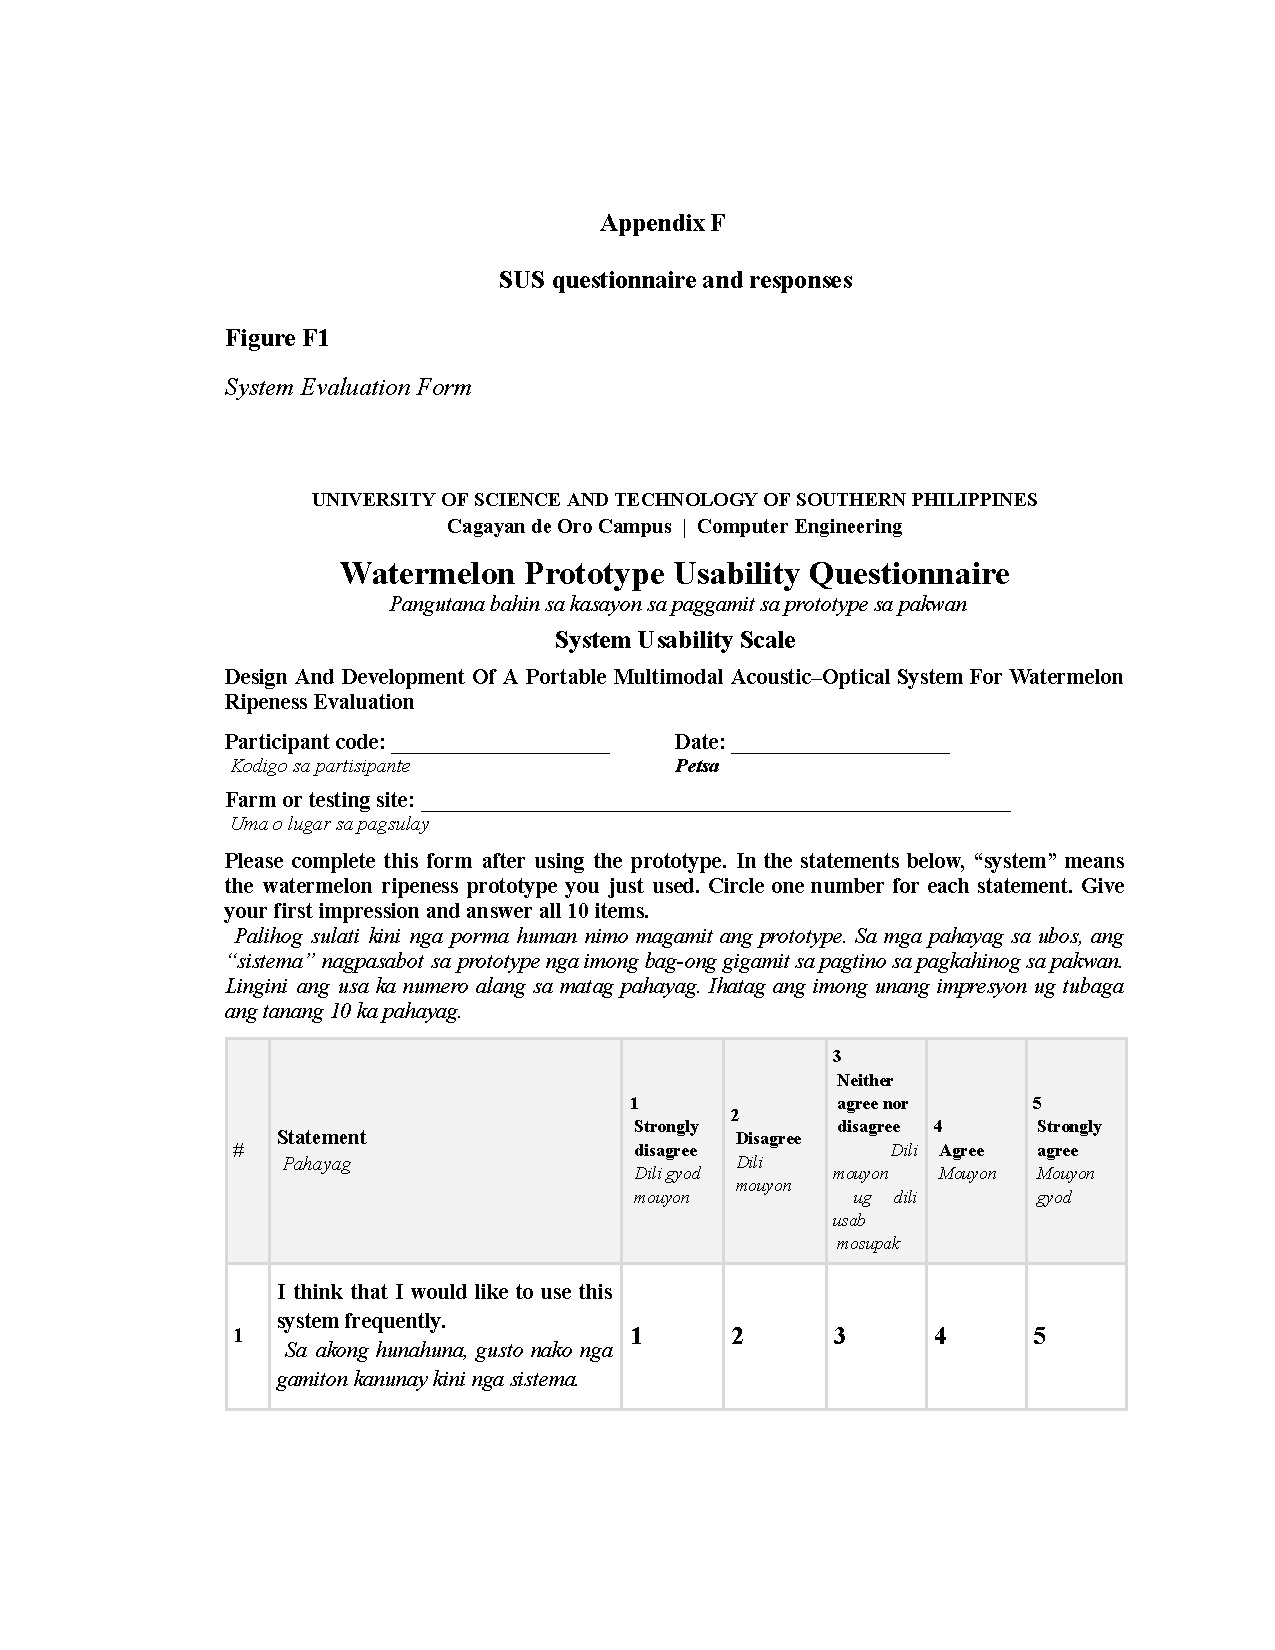
\includepdf[noautoscale,pages={1},pagecommand={\thispagestyle{empty}\phantomsection\csname defappvalue\endcsname{F1}\label{app:figure-F1}},addtotoc={1,section,1,{Appendix F. SUS questionnaire and responses},app:section-F}]{figures/appendix-records.pdf}

\includepdf[noautoscale,pages={2-3},pagecommand={\thispagestyle{empty}}]{figures/appendix-records.pdf}
\includepdf[noautoscale,pages={4},pagecommand={\thispagestyle{empty}},picturecommand={\setlength{\unitlength}{1bp}\put(294.04,522.60){\hyperlink{cite.brooke1996}{\phantom{\rule{49.79bp}{9.41bp}}}}}]{figures/appendix-records.pdf}
\includepdf[noautoscale,pages={5},pagecommand={\thispagestyle{empty}}]{figures/appendix-records.pdf}
\includepdf[noautoscale,pages={6},pagecommand={\thispagestyle{empty}},picturecommand={\setlength{\unitlength}{1bp}\put(139.99,134.28){\hyperlink{cite.brooke1996}{\phantom{\rule{65.99bp}{9.97bp}}}}}]{figures/appendix-records.pdf}
\includepdf[noautoscale,pages={7-26},pagecommand={\thispagestyle{empty}}]{figures/appendix-records.pdf}

\clearpage
\FloatBarrier\begin{landscape}
\appendixexhibit{table}{F1}{System Usability Scale Tally per Questions}
\begingroup
\footnotesize
\setlength{\tabcolsep}{3pt}
\renewcommand{\arraystretch}{1.14}
\setlength{\arrayrulewidth}{1.125pt}
\def\LTcaptype{uncaptionedgrid}
\begin{longtable}{|>{\centering\arraybackslash}p{\dimexpr 0.08446\linewidth-2\tabcolsep-2.25pt\relax}|>{\raggedright\arraybackslash}p{\dimexpr 0.35618\linewidth-2\tabcolsep-1.125pt\relax}|>{\centering\arraybackslash}p{\dimexpr 0.09058\linewidth-2\tabcolsep-1.125pt\relax}|>{\centering\arraybackslash}p{\dimexpr 0.08201\linewidth-2\tabcolsep-1.125pt\relax}|>{\centering\arraybackslash}p{\dimexpr 0.10404\linewidth-2\tabcolsep-1.125pt\relax}|>{\centering\arraybackslash}p{\dimexpr 0.09302\linewidth-2\tabcolsep-1.125pt\relax}|>{\centering\arraybackslash}p{\dimexpr 0.11628\linewidth-2\tabcolsep-1.125pt\relax}|>{\centering\arraybackslash}p{\dimexpr 0.07344\linewidth-2\tabcolsep-1.125pt\relax}|}
\hline
\cellcolor[HTML]{CFE2F3}{\bfseries Number} & \multicolumn{1}{>{\centering\arraybackslash}p{\dimexpr 0.35618\linewidth-2\tabcolsep-1.125pt\relax}|}{\cellcolor[HTML]{CFE2F3}{\bfseries Questions}} & \cellcolor[HTML]{CFE2F3}{\bfseries 1} & \cellcolor[HTML]{CFE2F3}{\bfseries 2} & \cellcolor[HTML]{CFE2F3}{\bfseries 3} & \cellcolor[HTML]{CFE2F3}{\bfseries 4} & \cellcolor[HTML]{CFE2F3}{\bfseries 5} & \cellcolor[HTML]{CFE2F3}{\bfseries Total Row} \\
\cline{3-7}
\endfirsthead
\hline
\cellcolor[HTML]{CFE2F3}{\bfseries Number} & \multicolumn{1}{>{\centering\arraybackslash}p{\dimexpr 0.35618\linewidth-2\tabcolsep-1.125pt\relax}|}{\cellcolor[HTML]{CFE2F3}{\bfseries Questions}} & \cellcolor[HTML]{CFE2F3}{\bfseries 1} & \cellcolor[HTML]{CFE2F3}{\bfseries 2} & \cellcolor[HTML]{CFE2F3}{\bfseries 3} & \cellcolor[HTML]{CFE2F3}{\bfseries 4} & \cellcolor[HTML]{CFE2F3}{\bfseries 5} & \cellcolor[HTML]{CFE2F3}{\bfseries Total Row} \\
\cline{3-7}
\endhead
\multicolumn{1}{|>{\raggedright\arraybackslash}p{\dimexpr 0.08446\linewidth-2\tabcolsep-2.25pt\relax}|}{\cellcolor[HTML]{CFE2F3}} & \cellcolor[HTML]{CFE2F3} & \cellcolor[HTML]{F4CCCC}Strongly Disagree & \cellcolor[HTML]{FCE5CD}Disagre & \cellcolor[HTML]{CCCCCC}Neither Agree nor Disagree & \cellcolor[HTML]{FFE599}Agree & \cellcolor[HTML]{B6D7A8}Strongly Agree & \multicolumn{1}{>{\raggedright\arraybackslash}p{\dimexpr 0.07344\linewidth-2\tabcolsep-1.125pt\relax}|}{\cellcolor[HTML]{CFE2F3}} \\
\hline
1 & I think that I would like to use this system frequently. \textit{(Sa akong hunahuna, gusto nako nga gamiton kanunay kini nga sistema.)} & 0 & 0 & 5 & 15 & 0 & 20 \\
\hline
2 & I found the system unnecessarily complex. \textit{(Para nako, mas komplikado ang sistema kaysa gikinahanglan.)} & 3 & 17 & 0 & 0 & 0 & 20 \\
\hline
3 & I thought the system was easy to use. \textit{(Para nako, sayon ra gamiton ang sistema.)} & 0 & 0 & 0 & 17 & 3 & 20 \\
\hline
4 & I think that I would need the support of a technical person to be able to use this system. \textit{(Sa akong hunahuna, kinahanglan nako ang tabang sa usa ka tawo nga adunay teknikal nga kahibalo aron magamit nako kini nga sistema.)} & 0 & 19 & 1 & 0 & 0 & 20 \\
\hline
5 & I found the various functions in this system were well integrated. \textit{(Para nako, maayo ang pagkahiusa sa nagkalainlaing mga gimbuhaton niini nga sistema.)} & 0 & 0 & 1 & 15 & 4 & 20 \\
\hline
6 & I thought there was too much inconsistency in this system. \textit{(Para nako, daghan kaayong dili magkatakdo sa paagi sa paglihok niini nga sistema.)} & 3 & 10 & 7 & 0 & 0 & 20 \\
\hline
7 & I would imagine that most people would learn to use this system very quickly. \textit{(Sa akong hunahuna, kadaghanan sa mga tawo dali ra kaayong makakat-on sa paggamit niini nga sistema.)} & 0 & 0 & 0 & 20 & 0 & 20 \\
\hline
8 & I found the system very cumbersome to use. \textit{(Para nako, hasol kaayo gamiton ang sistema.)} & 4 & 15 & 1 & 0 & 0 & 20 \\
\hline
9 & I felt very confident using the system. \textit{(Kompyansa kaayo ko sa akong paggamit sa sistema.)} & 0 & 0 & 0 & 20 & 0 & 20 \\
\hline
10 & I needed to learn a lot of things before I could get going with this system. \textit{(Kinahanglan pa nako nga makat-on og daghang butang sa dili pa ko makasugod sa paggamit niini nga sistema.)} & 3 & 17 & 0 & 0 & 0 & 20 \\
\hline
\multicolumn{2}{|>{\centering\arraybackslash}p{\dimexpr 0.44064\linewidth-2\tabcolsep-2.25pt\relax}|}{\cellcolor[HTML]{CFE2F3}Total Column} & 10 & 42 & 15 & 123 & 10 & 200 \\
\hline
\end{longtable}
\endgroup
\end{landscape}



\includepdf[noautoscale,pages={29-74},pagecommand={\thispagestyle{empty}},addtotoc={29,section,1,{Appendix G. Interview Guide},app:section-G}]{figures/appendix-records.pdf}

\includepdf[noautoscale,pages={75-76},pagecommand={\thispagestyle{empty}},addtotoc={75,section,1,{Appendix H. Nomination of Members of Oral Examination Panel Form},app:section-H}]{figures/appendix-records.pdf}

\includepdf[noautoscale,pages={77-80},pagecommand={\thispagestyle{empty}},addtotoc={77,section,1,{Appendix I. Application for Oral Defense of Thesis Forms},app:section-I}]{figures/appendix-records.pdf}

\includepdf[noautoscale,pages={81-82},pagecommand={\thispagestyle{empty}},addtotoc={81,section,1,{Appendix J. Approval Sheet for Hardbound Form},app:section-J}]{figures/appendix-records.pdf}

\endgroup

\fi

\thesisappendix{K}{Consultation Documentation}

\begin{figure}[htbp]
\appendixexhibit{figure}{K1}{September 4, 2026 Consultation}
{\centering 
\includegraphics[width=0.980\linewidth,height=.66\textheight,keepaspectratio]{\detokenize{figures/appendix-record-195.jpg}}\par}
\end{figure}

\begin{figure}[htbp]
\appendixexhibit{figure}{K2}{September 9, 2026 Consultation}
{\centering 
\includegraphics[width=0.980\linewidth,height=.66\textheight,keepaspectratio]{\detokenize{figures/consultation-k2-231.png}}\par}
\end{figure}

\begin{figure}[htbp]
\appendixexhibit{figure}{K3}{September 18, 2026 Consultation}
{\centering 
\includegraphics[width=0.980\linewidth,height=.66\textheight,keepaspectratio]{\detokenize{figures/consultation-k3-232.png}}\par}
\end{figure}

\begin{figure}[htbp]
\appendixexhibit{figure}{K4}{September 23, 2026 Consultation}
{\centering 
\includegraphics[width=0.980\linewidth,height=.66\textheight,keepaspectratio]{\detokenize{figures/consultation-k4-233.png}}\par}
\end{figure}

\begin{figure}[htbp]
\appendixexhibit{figure}{K5}{September 30, 2026 Consultation}
{\centering 
\includegraphics[width=0.490\linewidth,height=.66\textheight,keepaspectratio]{\detokenize{figures/consultation-k5-234.png}}\hfill\includegraphics[width=0.490\linewidth,height=.66\textheight,keepaspectratio]{\detokenize{figures/consultation-k5-235.png}}\par}
\end{figure}

\begin{figure}[htbp]
\appendixexhibit{figure}{K6}{October 1, 2026 Consultation}
{\centering 
\includegraphics[width=0.490\linewidth,height=.66\textheight,keepaspectratio]{\detokenize{figures/consultation-k6-236.png}}\hfill\includegraphics[width=0.490\linewidth,height=.66\textheight,keepaspectratio]{\detokenize{figures/consultation-k6-237.png}}\par}
\end{figure}

\begin{figure}[htbp]
\appendixexhibit{figure}{K7}{October 12, 2026 Consultation}
{\centering 
\includegraphics[width=0.490\linewidth,height=.66\textheight,keepaspectratio]{\detokenize{figures/consultation-k7-238.png}}\hfill\includegraphics[width=0.490\linewidth,height=.66\textheight,keepaspectratio]{\detokenize{figures/consultation-k7-239.png}}\par}
\end{figure}

\begin{figure}[htbp]
\appendixexhibit{figure}{K8}{October 12, 2026 Consultation}
{\centering 
\includegraphics[width=0.490\linewidth,height=.66\textheight,keepaspectratio]{\detokenize{figures/consultation-k8-240.png}}\hfill\includegraphics[width=0.490\linewidth,height=.66\textheight,keepaspectratio]{\detokenize{figures/consultation-k8-241.png}}\par}
\end{figure}

\begin{figure}[htbp]
\appendixexhibit{figure}{K9}{November 13, 2026 Consultation}
{\centering 
\includegraphics[width=0.490\linewidth,height=.66\textheight,keepaspectratio]{\detokenize{figures/consultation-k9-242.png}}\hfill\includegraphics[width=0.490\linewidth,height=.66\textheight,keepaspectratio]{\detokenize{figures/consultation-k9-243.png}}\par}
\end{figure}

\begin{figure}[htbp]
	\appendixexhibit{figure}{K10}{November 26, 2026 Consultation}
	{\centering 
		\includegraphics[width=0.490\linewidth,height=.66\textheight,keepaspectratio]{\detokenize{figures/consultation-k10-244.jpg}}\hfill\includegraphics[width=0.490\linewidth,height=.66\textheight,keepaspectratio]{\detokenize{figures/consultation-k10-245.jpg}}\par}
\end{figure}

\begin{landscape}
\thesisappendix{L}{Gantt Chart}

\begin{figure}[H]
\appendixexhibit{figure}{L1}{Second Semester, 3rd Year (January to May)}
{\centering 
\includegraphics[width=0.980\linewidth,height=.53\paperwidth,keepaspectratio]{\detokenize{figures/gantt-chart-244.png}}\par}
\end{figure}

\newpage

\begin{figure}[H]
\appendixexhibit{figure}{L2}{First Semester, 4th Year (June to November)}
{\centering
\includegraphics[width=0.980\linewidth,height=.53\paperwidth,keepaspectratio]{\detokenize{figures/gantt-chart-245.png}}\par}
\end{figure}

\end{landscape}

\endgroup
